\documentclass[12pt]{article}

\usepackage{palatino}   % Pretty Font
\usepackage{amsmath}    % American Mathematical Society (AMS) commands
\usepackage{amsthm}     % AMS Theorem commands
\usepackage{amssymb}    % AMS Symbols
\usepackage{semantic}   % Tools for typesetting PL semantics
\usepackage{fancyhdr}   % header/footer for each page
% \usepackage[margin=1in]{geometry}   % Give me reasonable margins
\usepackage{braket}     % Easy angle-bracket notation
\usepackage{mathpartir} % Used to typeset blocks of inference rules
%\usepackage[usenames,dvipsnames]{color}      % for colors
\usepackage[usenames]{color}      % for colors
\usepackage{rotating} % for sidewaysfigure
\usepackage{proof}
\usepackage{datetime}
\usepackage{pdflscape}
\usepackage{fancyvrb} % to use \verb in footnotes
\usepackage{enumitem} %% for resuming enumerations
\usepackage{stmaryrd}
\usepackage{natbib}

\usepackage{fullpage}
\usepackage{framed}
\usepackage{dsfont}
\usepackage{latexsym}
\usepackage{amsfonts}
\usepackage{mathrsfs}
\usepackage{aliascnt}
% \usepackage{pstricks}
% \usepackage{pst-all}
% \usepackage{pstricks-add}
% \usepackage{pst-plot}
\usepackage[title]{appendix}
\usepackage{graphicx}
% \usepackage{subfig}
% \usepackage{enumerate}
\PassOptionsToPackage{hyphens}{url}\usepackage[pdfpagelabels,pdfpagemode=None]{hyperref}

% \usepackage{algorithmic}
\usepackage{mathtools}
\usepackage{algorithm}
\usepackage{algpseudocode}
\usepackage[dvipsnames]{xcolor}
\usepackage{tikz}
\usepackage[font=small,labelfont=bf]{caption}
\usepackage{subcaption}
\usepackage{bold-extra}

\usetikzlibrary{positioning,chains,fit,shapes,calc,arrows.meta,arrows,automata,decorations.text}


\newcommand{\rbsf}[1]{\textsf{\color{red}#1}}
\reservestyle{\errlang}{\rbsf}

\errlang{mismatch,underflow,unbound}


% Finite partial map
\newcommand{\finto}{\stackrel{\text{fin}}{\rightharpoonup}}
\newcommand{\pto}{\rightharpoonup}
\newcommand{\len}[1]{\lvert {#1} \rvert}

\theoremstyle{plain}
\newtheorem{theorem}{Theorem}
\newtheorem{lemma}{Lemma}
\newtheorem{proposition}{Proposition}
\newtheorem{conjecture}{Conjecture}
\newtheorem{corollary}{Corollary}
\newtheorem{definition}{Definition}
\newtheorem{problem}{Problem}

\theoremstyle{definition}
\newtheorem{example}{Example}

% When a property is true by the Induction Hypothesis...
\newcommand{\ih}[1]{\stackrel{\text{I.H.}}{#1}}


\theoremstyle{remark}
\newtheorem*{case}{Case}
\newtheorem*{note}{Note}
\newtheorem*{notation}{Notation}
\newtheorem*{solution}{Solution}
\newenvironment{subcase}[1][]{
  \mbox{}\\\mbox{}\quad
  \begin{minipage}{1.0\linewidth}
    \begin{case}[#1]
      }{
    \end{case}
  \end{minipage}
}

% The following helps fix having too much vertical space when writing
% predicates or functions applied to derivation trees
\newcommand{\sarray}[1]{
  {\begin{array}[c]{@{}l@{}} #1
      \end{array}}}

\newcommand{\fdeduce}[2]{\ensuremath{#2 :: #1}}

%% Random math macros

% Set Theory
\newcommand{\tuple}[1]{\braket{#1}}
\newcommand{\setint}{\ensuremath{\cap}}
\newcommand{\setdiff}{\mathrel{\backslash}}
\newcommand{\union}{\ensuremath{\cup}}   % the set union symbol
\newcommand{\Z}{\ensuremath{\mathbb{Z}}} % the set of integers
\newcommand{\N}{\ensuremath{\mathbb{N}}} % the set of naturals
\newcommand{\B}{\ensuremath{\mathbb{B}}} % the set of booleans
\newcommand{\R}{\ensuremath{\mathbb{R}}}
\newcommand{\Pow}{\ensuremath{\mathcal{P}}} % The powerset

% Logic
%\renewcommand{\land}{\mathop{{\wedge}}}
\newcommand{\limplies}{\mathop{{=>}}}
\newcommand{\ltrue}{{\top}}
%\renewcommand{\lor}{\mathop{{\vee}}}
\newcommand{\lfalse}{{\bot}}
\newcommand{\lequiv}{\mathop{{\equiv}}}



%% Comments
\newcommand{\comment}[2]{{\color{red}[{\sc #1:} \textsf{#2}]}}
%\renewcommand{\comment}[2]{}
\newcommand{\ron}[1]{\comment{RG}{#1}}


%%
%% Macros for syntax definitions
%%
\newcommand{\mvar}[1]{\ensuremath{\mathit{#1}}}
\newcommand{\seq}[1]{\ensuremath{\overline{#1}}}
\newcommand{\hole}{\square}
\newcommand{\nsubst}[3]{{[#2 \Mapsto #1]#3}}
\newcommand{\ansubst}[3]{{\underline{[#2 \Mapsto #1]}#3}}

%ron Redefine \subst
\newcommand{\subst}[3]{\ensuremath{[#1/#2]#3}}
\newcommand{\asubst}[3]{\ensuremath{\underline{[#1/#2]}#3}}
\newcommand{\remap}[3]{\ensuremath{#1[#2 \mapsto #3]}}


%%
%% inferbox: an environment for typesetting a group of inference rules
%%
\newenvironment{inferbox}[1][\textwidth]
{\begin{minipage}{#1}\begin{mathpar}}
      {\end{mathpar}\end{minipage}}


%% buinfer: build an inference tree bottom up, rather than top-down.  Sometimes
%% this is easier to do, especially when building complicated trees

\newcommand{\binference}[3][]{\inference[#1]{#3}{#2}}
%\newcommand{\binference}[3][]{\infer[\text{#1}]{#2}{#3}}

% silent inference - ignore the labels
\newcommand{\sinference}[3][]{\inference[]{#2}{#3}}

% Derivation-related macros
\newcommand{\D}{\mathcal{D}}
\newcommand{\E}{\mathcal{E}}
\newcommand{\F}{\mathcal{F}}
\newcommand{\ddd}{\raisebox{0.2em}[1.1em]{$\vdots$}}


%% block - used to indent code or create newlines of math stuff.
\newenvironment{block}[1][t]
{\begin{array}[#1]{@{}l@{}}}
    {\end{array}}

% Block, or any array[t]/array[c]/array[b] does not play well with 
% stretchy parens or brackets.  Use this instead.
% It protects everything in another array
\newenvironment{roundbrack}{\left(\begin{array}{@{}l@{}}}
    {\end{array}\right)}


% mark something in gray outline
\definecolor{lightgray}{gray}{0.80}
\newcommand{\Gbox}[1]{\colorbox{lightgray}{$#1$}}

\newcommand{\gbox}[1]{{\setlength{\fboxsep}{0pt}\colorbox{lightgray}{#1}}}

%% Math ligatures (thanks to the semantic package) that make it
%% easier to typeset math using readable LaTeX text.
\mathlig{|-->}{\longmapsto}
\mathlig{[]}{\square}
\mathlig{||}{\mathrel{\color{black}\Downarrow}}
\mathlig{!!}{{\color{blue}!}}
\mathlig{;;}{\mbsf{;}}
\mathlig{::==}{\mathbin{\color{blue}\texttt{\bf \upshape :=}}}
%\mathlig{::==}{\mbsf{:=}}
\mathlig{|}{\mid}
\mathlig{..}{{\color{blue}.}}
\mathlig{@-}{\mathbin{\color{blue}\texttt{\bf \upshape -}}}
\mathlig{++}{\mathbin{\color{blue}\texttt{\bf \upshape +}}}
\mathlig{**}{\mathbin{\color{blue}\mathbf{*}}}
\mathlig{==}{\mathbin{\color{blue}\texttt{\bf \upshape =}}}
\mathlig{,,}{{\color{blue},}}
\mathlig{[[}{\mbsf{[}}
\mathlig{]]}{\mbsf{]}}
\mathlig{@:}{\mbsf{:}}
\mathlig{@(}{{\color{blue}\texttt{\bf \upshape (}}}
\mathlig{@)}{{\color{blue}\texttt{\bf \upshape )}}}
%\mathlig{@(}{\mbsf{(}}
%\mathlig{)@}{\mbsf{)}}
\newcommand{\tbrack}[1]{{\triangleleft#1\triangleright}}
\newcommand{\thunk}[1]{\tbrack{\hspace{2pt}#1\hspace{2pt}}}
\newcommand{\closure}{\texttt{\textbf{\#<closure>}}}

\newcommand{\unit}{{\color{blue}\texttt{\bf ()}}}


% Use smallcaps for the names of object language sets.
\newcommand{\oblset}[1]{\textsc{#1}}

% Some common Sets
\newcommand{\TreeSet}{\oblset{Tree}}
\newcommand{\Tree}{\oblset{Tree}}
\newcommand{\Deriv}{\oblset{Deriv}}
\newcommand{\Term}{\oblset{Term}}
\newcommand{\Value}{\oblset{Value}}
\newcommand{\Var}{\oblset{Var}}
\newcommand{\Pgm}{\oblset{Pgm}}
\newcommand{\Obs}{\oblset{Obs}}
\newcommand{\Frame}{\oblset{Frame}}
\newcommand{\ECtxt}{\oblset{ECtxt}}
\newcommand{\Ctxt}{\oblset{Ctxt}}
\newcommand{\Redex}{\oblset{Redex}}
\newcommand{\Type}{\oblset{Type}}

% Some custom notations for the metalanguage
\reservestyle{\mtlang}{\textit}
\renewcommand{\eval}{\mathit{eval}}
\newcommand{\dom}{\mathit{dom}}
\newcommand{\cod}{\mathit{cod}}
\newcommand{\unload}{\mathit{unload}}

% Some custom notations for object language stuff
% Typeset object language notation in blue with sans serif font
\newcommand{\blue}[1]{{{\color{blue}#1}}}
\newcommand{\tbsf}[1]{\textsf{\color{blue}#1}}
\newcommand{\mbsf}[1]{\mathsf{\color{blue}#1}}
\newcommand{\ol}[1]{\ensuremath{\mbsf{#1}}}
\reservestyle{\oblang}{\tbsf}



%
% Languages:
%

% Logic
% RG: This is actually metalanguage:  there is a logic object language which 
% should go here.  Move Logic up

% Formalized
\newcommand{\band}{\mathop{\mbsf{\wedge}}}
\newcommand{\bimplies}{\mathop{\mbsf{=>}}}
\newcommand{\btrue}{\mbsf{\top}}
\newcommand{\bor}{\mathop{\mbsf{\vee}}}
\newcommand{\bnot}{\mathop{\mbsf{\lnot}}}
\newcommand{\bfalse}{\mbsf{\bot}}
\newcommand{\bequiv}{\mathop{\mbsf{\equiv}}}

\newcommand{\jtrue}{\textbf{true}}



% Booleans
\newcommand{\Bool}{\oblset{Bool}}
\oblang{if-then-else[if],true,false,if[if\;],then[\;then\;],else[\;else\;]
}


% Arithmetic
% RG: Why do I have both Num and Nat?
\newcommand{\Num}{\oblset{Num}}
\oblang{z,succ,pred,zero?}
\newcommand{\nv}{\mathit{nv}}


% IMP <: Booleans
\newcommand{\AExp}{\oblset{AExp}}
\newcommand{\BExp}{\oblset{BExp}}
\newcommand{\Com}{\oblset{Com}}
\newcommand{\Env}{\oblset{Env}}
\newcommand{\DO}{\oblset{DO}}
\newcommand{\Store}{\oblset{Store}}
\newcommand{\SO}{\oblset{SO}}
\newcommand{\Loc}{\oblset{Loc}}
\newcommand{\PLOC}{\Pow(\Loc)}
\newcommand{\ACfg}{\oblset{ACfg}}
\newcommand{\BCfg}{\oblset{BCfg}}
\newcommand{\CCfg}{\oblset{CCfg}}

\oblang{while[while\;],do[\;do\;],skip}

\newcommand{\X}{\mbsf{X}}
\newcommand{\Y}{\mbsf{Y}}
\newcommand{\ZZ}{\mbsf{Z}}

\newcommand{\bv}{\mathit{bv}}
\newcommand{\bsa}{\Downarrow_{\AExp}}
\newcommand{\bsb}{\Downarrow_{\BExp}}
\newcommand{\bsc}{\Downarrow_{\Com}}

\newenvironment{whileblock}[2][t]
{\begin{block}[#1]\<while> \mbsf{#2} \<do>\\
    \quad\begin{block} \color{blue}}
      {\end{block}\end{block}}


% Doesn't work because of the end-environment part (grr...)
% \newenvironment{doblock}[2][t]
%   {\begin{block}[#1]\<do>\\
%       \quad\begin{block} \color{blue}}
%     {\end{block} \<while> \mbsf{#2} \end{block}}



% Procedures (Lambda Calculus)
\newcommand{\blambda}{\ensuremath{{\color{blue}\lambda}}}
\newcommand{\FV}{\mathit{FV}}
\newcommand{\BV}{\mathit{BV}}
\newcommand{\Vars}{\mathit{Vars}}
\newcommand{\Locs}{\mathit{Locs}}
\oblang{var,apply,procedure}
\oblang{tlet[let],let[let\;],dlet[dlet\;],in[\;in\;],nin[in\;]}

\newcommand{\w}{\mbsf{w}}
\newcommand{\x}{\mbsf{x}}
\newcommand{\y}{\mbsf{y}}
\newcommand{\z}{\mbsf{z}}

\newenvironment{letblock}[2][t]
{\begin{block}[#1]\<let> \mbsf{#2} \\
    \<nin>\begin{block} \color{blue}}
      {\end{block}\end{block}}


% Recursion
\oblang{fix[fix\;],rec[rec\;]}

\newenvironment{fixblock}[2][t]
{\begin{block}[#1]\<fix> \mbsf{#2}. \\
    \quad\begin{block} \color{blue}}
      {\end{block}\end{block}}


% Unit
\oblang{unit,Unit}

% References
\oblang{ref[ref\;]}


% Exceptions
\oblang{raise[raise\;],try[try\;],handle[\;handle\;]}

% Continations
% use \braket{E} for continuation values
\oblang{letcc[let/cc\;],throw[throw\;]}

\newenvironment{letccblock}[2][t]
{\begin{block}[#1]\<letcc> \mbsf{#2} \\
    \<nin>\begin{block} \color{blue}}
      {\end{block}\end{block}}


% Pairs
\newcommand{\pr}[2]{\mbsf{(}#1\mbsf{,\,}#2\mbsf{)}}
\oblang{fst[fst\;],snd[snd\;]}


% Sums
\oblang{inr,inl,case[case\;],of[\;of]}

\newcommand{\tcase}[5]{
  \begin{block}
    \<case> #1 \<of> \\
    \quad
    \begin{block}
      \<inl>\;#2  .. #3 \\
      \<inr>\;#4  .. #5 \\
    \end{block}
  \end{block}
}


% Recursive Types
\oblang{fold,unfold}

% Errors
\oblang{error}



%
% Other stuff
%

% CPS translation function
\newcommand{\cps}[1]{|[ #1 |]}


%%% Local Variables: 
%%% mode: latex
%%% TeX-master: t
%%% End: 

% Algorithms
\newcommand{\matroid}{\mathcal{M}}
\newcommand{\classp}{\mathsf{P}}
\newcommand{\classnp}{\mathsf{NP}}
\newcommand{\classnpo}{\mathsf{NPO}}
\newcommand{\yes}{\mathsf{YES}}
\newcommand{\no}{\mathsf{NO}}
\newcommand{\preduce}{\leq_{\classp}}
\newcommand{\ALGO}{\mathcal{A}}
\newcommand{\alg}{\mathsf{ALG}}
\newcommand{\opt}{\mathsf{OPT}}
\newcommand{\eps}{\epsilon}
\newcommand{\equal}{\texttt{\,=\,}}
\let\oldemptyset\emptyset
\let\emptyset\varnothing

\algrenewcommand\algorithmicrequire{Input:}
\algrenewcommand\algorithmicensure{Output:}
\algdef{SE}[SUBALG]{Indent}{EndIndent}{}{\algorithmicend\ }%
\algtext*{Indent}
\algtext*{EndIndent}

\renewcommand\proofname{\textsc{Proof.}}
\usepackage[normalem]{ulem}
\usepackage[paperheight=11.0in,paperwidth=8.5in,left=1.0in,right=1.0in,top=1.0in,bottom=1.0in,headheight=1in]{geometry}
\usepackage{url}

\tikzset{>={Latex[width=1.5mm,length=2mm]}}
\usepackage{listings}

\renewcommand{\baselinestretch}{1.3}
\renewcommand{\_}{\kern-1.5pt\textunderscore\kern-1.5pt}
\renewcommand{\arraystretch}{1.3}

\usepackage{array}
\usepackage{float}
\newcommand{\PreserveBackslash}[1]{\let\temp=\\#1\let\\=\temp}
\newcolumntype{C}[1]{>{\PreserveBackslash\centering}p{#1}}
\newcolumntype{R}[1]{>{\PreserveBackslash\raggedleft}p{#1}}
\newcolumntype{L}[1]{>{\PreserveBackslash\raggedright}p{#1}}

% \usepackage{multicol}

\lstset{basicstyle=\scriptsize\ttfamily,
  showstringspaces=false,
  commentstyle=\color{red},
  keywordstyle=\color{blue}
}

\title{SoliGity}
\author{  
  Roger Luo\\
  45323136
  \and
  Zhenpeng Wu\\
  28125152 
  \and
  Zitian Tong\\
  41439143
}

\date{\today}


\begin{document}

\maketitle

\section{Introduction}

Today, the open-source community is thriving rapidly, creating a synergistic environment to allow individuals
from all over the world to learn from each other and to create software that can create significant impacts.
Although much of open source work is volunteered, there are many reasons that an open-source developer deserves
rewards or incentives for their contributions, especially if the project is complex and time-consuming~\cite{community_collaboration}.

Apart from the complexity of an open-source project that rewarding mechanisms may apply, we suggest at one
particular group, students, also deserve incentives for their contributions. Research has found that open-source
projects play an important role in university students’ success~\cite{open_source_guides}. We surveyed 50
students majoring in EECS (Electrical Engineering and Computer Science), over 75\% of them consider finding
an internship job as one of their highest priorities. Standing out from a large pool of applicants, however,
requires students to work on side projects. Furthermore, over 50\% of the students find it difficult to discover
and identify the projects that interest them; even for those who do find an interesting project, 62\% of them
found it hard to stay motivated~\cite{thomas_toch_2014}. More importantly, the contributors of open-source
projects suggest they deserve more recognition for their work~\cite{freecodecamp.org_2018}.

Currently, getting paid or rewarded to work on open source projects still relies on a traditional form of funding
mechanism such as crowdfunding campaigns or sponsorships~\cite{open_source_guides}. These mechanisms, however,
involve a long chain of decision-making processes: First, the project owner/creators will post their projects
or ideas on a third-party platform such as OpenCollective, Patreon, and Rekonse. These platforms usually act
as a middleman, keeping a ledger between the sponsor and the project owner to inform each other how the money
flows. Then, the money raised from the crowd will go through multiple layers of committee members to identify
and decide which feature/issue the money should be spent on. The time it takes for the fund to reach a developer
is unnecessarily long. Depending on how the project is managed, it might not be transparent to the developers
that the fund from the sponsor is reasonably and fairly distributed, based on their share of contributions. More
importantly, these crowd-funding models only work well if the project is already very complex, well-known and
has a strong audience - it’s almost impossible to establish a fine-grained transaction between a developer and
a project owner on per-issue or per-feature bases. It is less likely for a broader group of community members
(e.g. students and entry-level developers) to get involved in these crowded-funded open-sources projects.
Furthermore, the transaction of the fund using conventional currencies (mostly USD) has to go through credit
card services, meaning that there are overheads such as currency exchange, processing time, and transaction fees.

In summary, we argue that there are two pain points in the open-source developer community:

\begin{enumerate}

	\item There is a lack of a unified, purposeful platform that provides an end-to-end experience to
	      help developers in the open-source community discover open-source projects to work on, especially
	      for entry-level developers.

	\item Getting paid or rewarded by working on open-source projects still relies on a conventional
	      crowd-funding/sponsorship model that does not achieve an optimal level of flexibility, efficiency,
	      security, and transparency.

\end{enumerate}

We attempt to address these pain points by leveraging web technologies, Git source control, and blockchain
decentralized application (DApp) to create a novel platform - SoliGity to establish a closer connection with
repository owners and contributors. Developers have the opportunities to discover interesting projects, make
contributions and get rewarded from the project owners.

Blockchain technologies are of a great fit to address these pain points - unlike a conventional centralized
ledger keeping track of the transaction, blockchain is a type of distributed ledger, all network participants
share the same ledger and the shared version can only be updated when everyone agrees on
it~\cite{blockchain_pulse_ibm_blockchain_blog_2020}. This ensures that the sponsor and the developer will have
accurate, consistent and transparent information on the transactions between them. Blockchain also increases
the efficiency and speed of trading, eliminating the need for third-party mediation and avoiding human error.
Unlike the traditional server-client architecture, where the server might shut down unexpectedly, a decentralized
blockchain system has no central point of failure, as it is being run from thousands of volunteers’ computers
around the globe, meaning that it can never go offline. For us, it means the management and maintenance costs
are dramatically reduced~\cite{thomas_toch_2014}. Blockchain also ensures the security and traceability of the
record-keeping.

Our project is developed based on the Ethereum (ETH) platform using a smart contract written in Solidity - an
object-oriented, high-level language for implementing smart contracts. As the second-largest cryptocurrency in
the world, ETH has the benefit of Bitcoin (BTC) but it further leverages the properties of decentralization by
introducing smart contracts and Ethereum virtual machine (EVM). Ethereum is a multipurpose platform where its
digital currency ETH is just a component of its smart contract application. In the subsequent sections we will
discuss in detail how we implement the DApp in Solidity in the context of Git workflow (hence our name SoliGity)
to achieve an efficient transaction workflow between the project owner and the developer.


\section{Use Case Workflow}
\label{section:usecaseworkflow}

SoliGity aims to provide a friendly, intuitive experience end-to-end in between the open-source project owner and the developers. It integrates with the Git seamlessly in the way that extra steps are minimized. Since it is a web-based platform with GitHub integration, both project owners and developers need to sign up for an account and associate it with their GitHub account prior to taking advantage of our services. Note that the account is general-purpose. A user can act as both the project owner and the developer using the same account - he/she can own a project and seek others’ help while helping with other people’s projects as developers. Our project also assumes that the user’s computer is properly configured with an Ethereum account as well as Meta Mask - A crypto wallet \& gateway that provides the user with a wallet to store and transact his/her Ethereum and Ethereum-based tokens through a web browser. \\

\noindent After signing up, the workflow can be summarised in four steps (Figure~\ref{fig:workflow1}):

\begin{figure}[H]
	\centering
	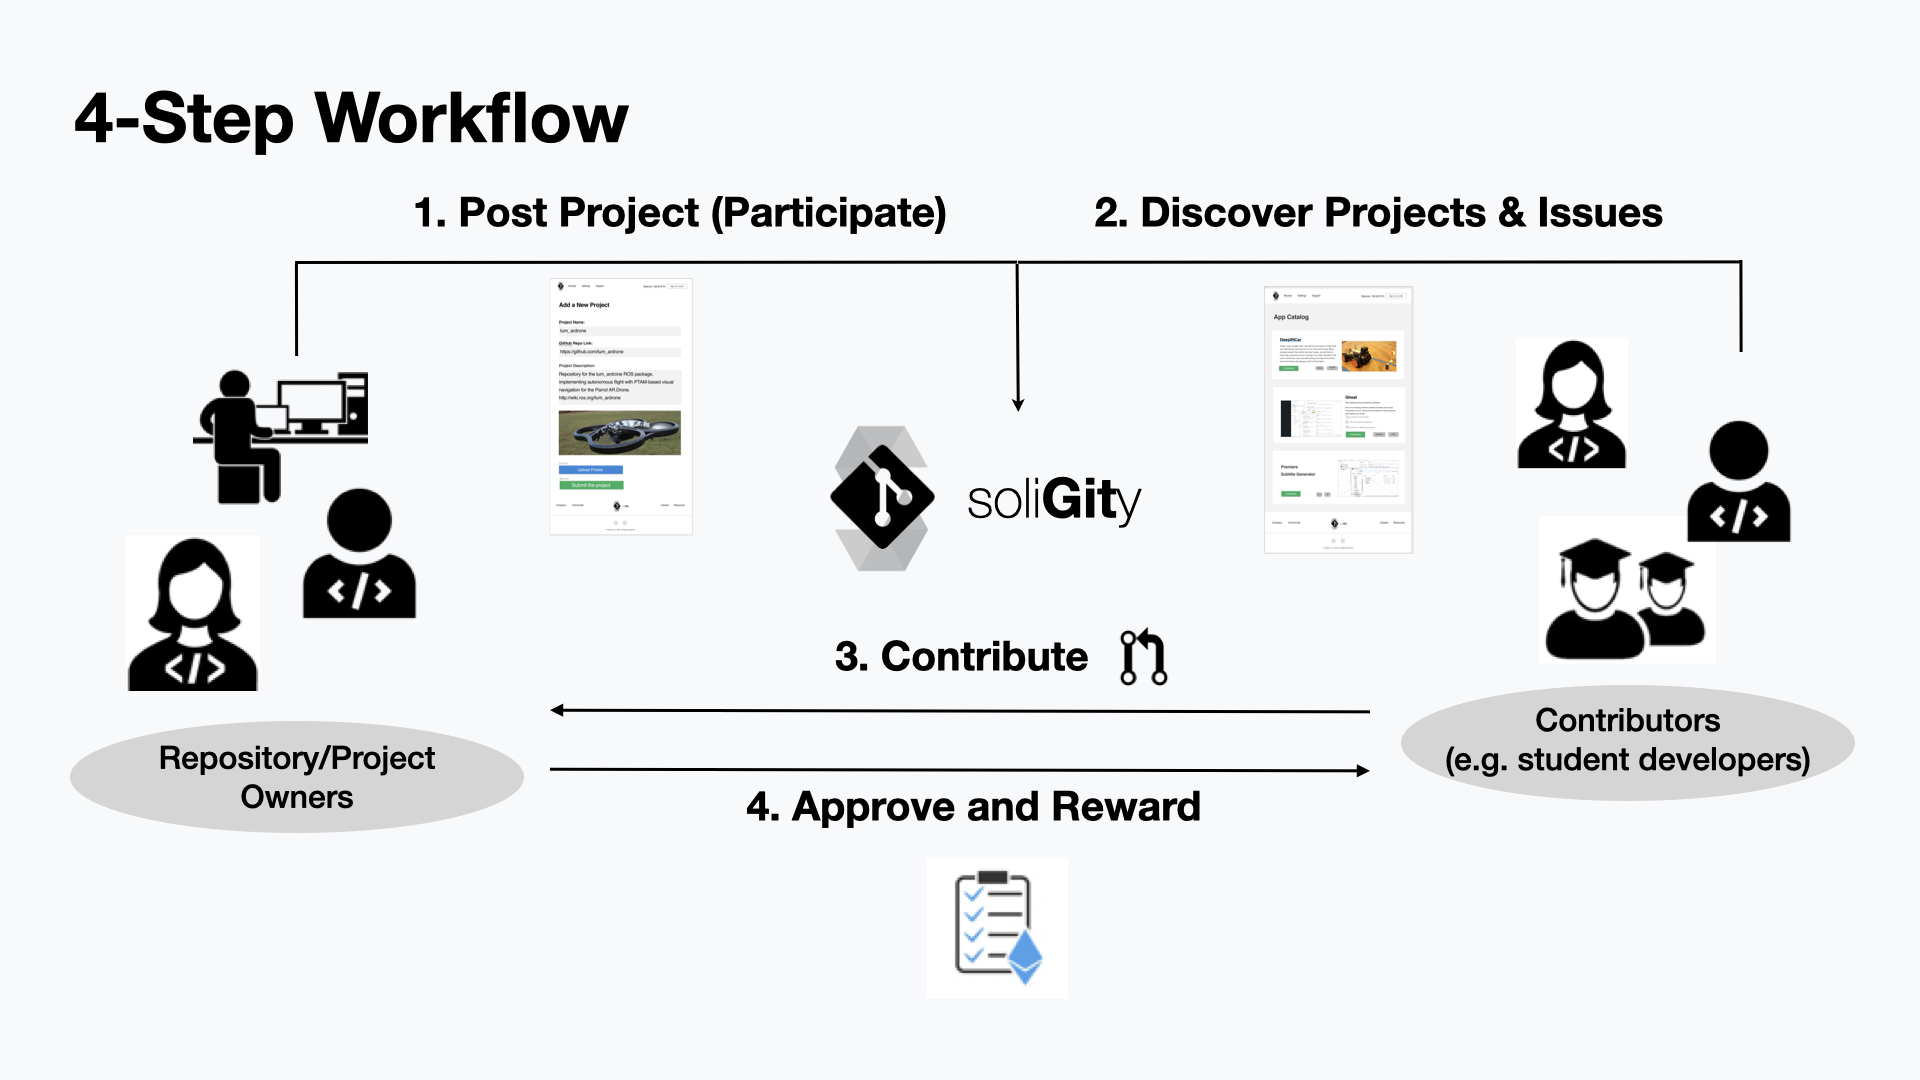
\includegraphics[width=16.5cm]{graphs/00a. workflow.jpeg}
	\caption{SoliGity 4-Step Workflow}
	\label{fig:workflow1}
\end{figure}



\renewcommand\thesubsection{Step \arabic{subsection}.}
\renewcommand\thesubsubsection{\arabic{subsubsection}.}

\subsection{Post Project}

As mentioned earlier, the SoliGity account is associated with the user’s GitHub account. Once configured, the user can access the list of their own repositories (Figure~\ref{fig:workflow2}a). To have one of their repositories being discovered by everyone on the platform, the project owner must link/add this repo to the project catalog (Figure~\ref{fig:workflow2}b). For every project in the catalog, any user can create issues (Figure~\ref{fig:workflow2}c). All issues created within SoliGity will be book-kept in the SoliGity blockchain DApp, and they will be propagated to GitHub as regular GitHub issues using GitHub APIs. While creating an issue, SoliGity also prompts the user for a price - the amount of cryptocurrency that the project owner will award to the developer when the work is approved. Each issue also comes with a status tracked by the DApp - \textit{Accepting Contributions}, \textit{Pending Approval}, and \textit{Done}. In this stage, a newly-opened issue is in \textit{Accepting Contribution} status.


\begin{figure}[H]
	\centering
	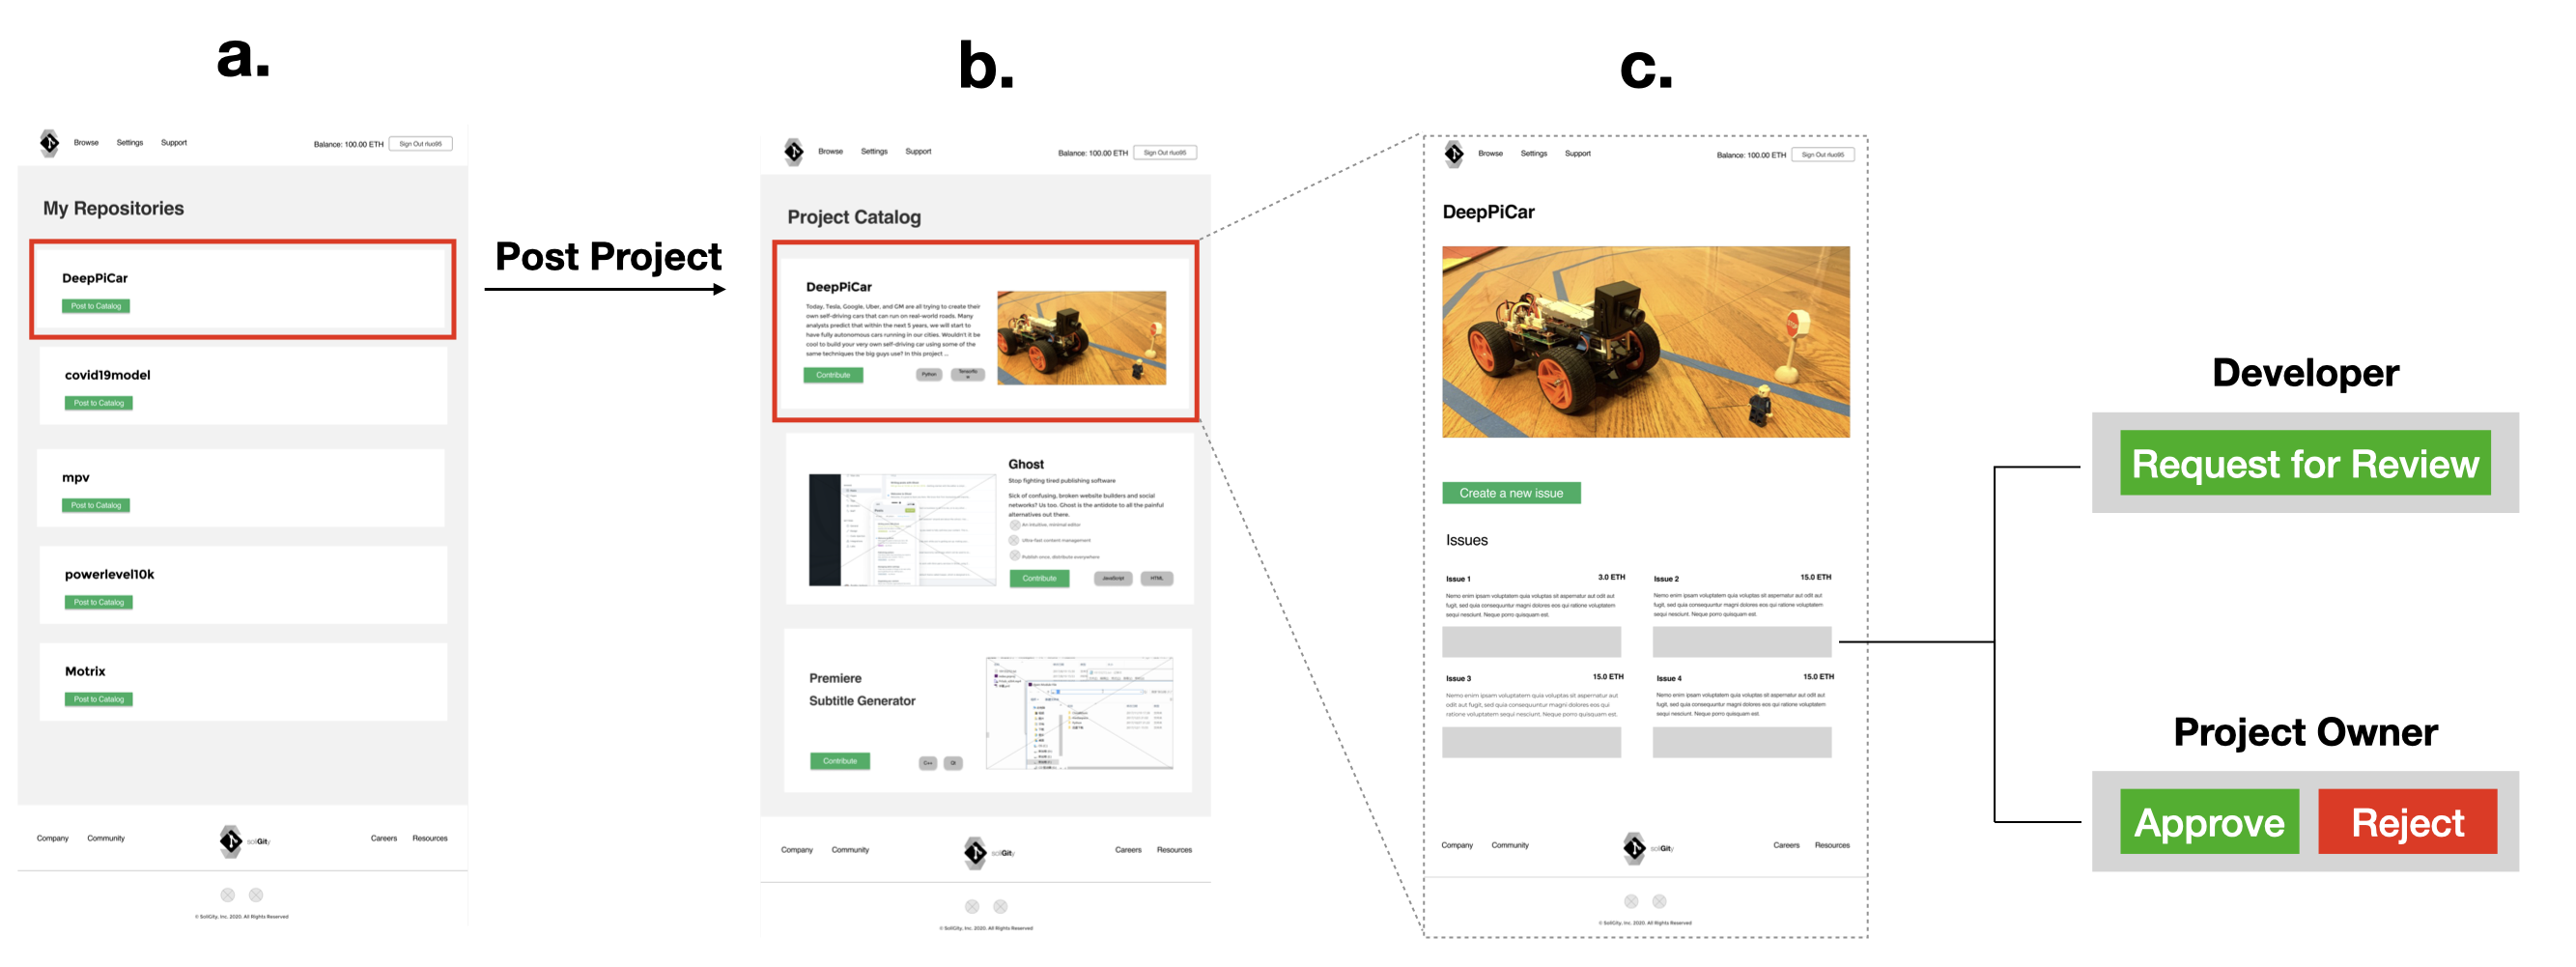
\includegraphics[width=16.5cm]{graphs/00b. workflow.png}
	\caption{SoliGity 4-Step Workflow}
	\label{fig:workflow2}
\end{figure}

\subsection{Discover Project}

Once the projects are posted on the catalog, everyone can discover them. We envision an interface that looks like an App Store, displaying project information in rich details such as project name, pictures, languages \& frameworks etc. The intuitive, friendly experience will be of great benefit for these entry-level developers and students to quickly become interested in a project. The project description page (Figure~\ref{fig:workflow2}c) displays the issues. Note that issues are not limited to bugs - they can also be new features and feasibility studies that’s available for anyone to pick up and make contributions.

\subsection{Making Contribution}

Once the developer finds an issue to work on, he/she must fork the repository to their own GitHub account. We provide a button shortcut to help the developer fork the repo without leaving SoliGity. Then, the development process is identical to regular Git workflow - the developer commits and pushes the work to their forked repo, then makes a pull request when the work is done (Figure~\ref{fig:workflow2}c). Note that the review request is made in SoliGity - this makes sure that both our DApp and GitHub are aware of this activity. On SoliGity, the issue status will be changed to \textit{Pending Approval} from \textit{Accepting Contribution}; on GitHub, a pull request will be made for the project owner to review the code changes.

\subsection{Rewarding Contribution}
When a review request is made, the project owner reviews the code changes on GitHub website as he/she normally does in the traditional Git workflow. If the work is acceptable, the owner will approve the code change on SoliGity by pressing the Approve button (Figure~\ref{fig:workflow2}c). Doing so will (i) Merge the changes to the owner’s Git repository;
(ii) Transfer the bounty in ETH to developer’s wallet;
(iii) Change the issue status from \textit{Pending Approval} to \textit{Done}. In case the owner is not satisfied with the code changes, he/she can reject the contribution by pressing the Reject button (Figure~\ref{fig:workflow2}c). This will set the issue status back to Accepting Contribution and the process can be re-started. The state transition diagram below visualizes three states of an issue.\\

   \begin{center}
   \scriptsize
      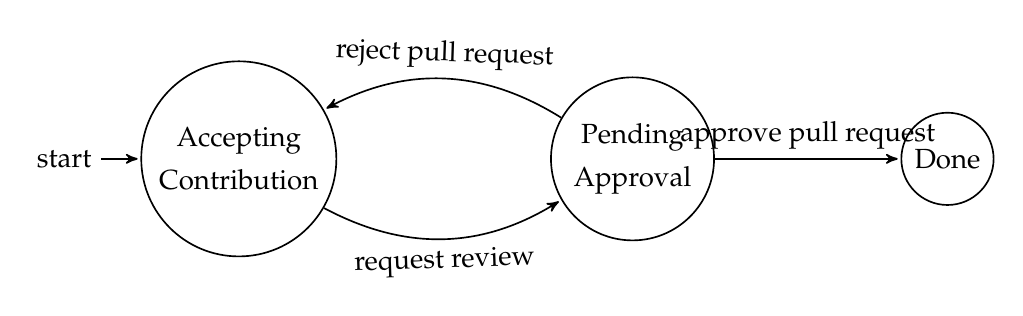
\begin{tikzpicture}[-,>=stealth',shorten >=1pt,auto,node distance=4cm,semithick]
        \tikzstyle{every state}=[text=black]

        \node[state, initial left, align=center] (a) {Accepting\\Contribution} ;
        \node[state, right of=a, align=center,xshift=1cm] (p) {Pending\\Approval};
        \node[state, right of=p, align=center] (d) {Done};
        \draw[->]

        (a) edge[bend right] node[sloped,below,align=center]{request review} (p)
        (p) edge[] node[sloped,above,align=center]{approve pull request} (d)
        (p) edge[bend right] node[sloped, above, align=center]{reject pull request} (a)
        ;

      \end{tikzpicture}
    \end{center}

\noindent Since the GitHub commands including Issue Creation, Fork, and Making Pull Request are fully integrated into SoliGity, the entire workflow is intuitive and straightforward. The transaction takes place between the project owner and the developer nearly instantly and securely without third parties. All of these functional and non-functional features make SoliGity redefine the open-source project rewarding mechanism. In the next section we demonstrate our working prototype step-by-step.

\section{Step-by-step Screenshot with Explanation}
In this section, we demonstrate SoliGity step-by-step.


\renewcommand\thesubsection{Step \arabic{subsection}.}
\renewcommand\thesubsubsection{\arabic{subsubsection}.}

\subsection*{Step 0. \(\;\;\)Initial Setup}

\subsubsection{Setup Environment}

% \begin{figure}[H]
% 	\begin{minipage}[t]{0.4\linewidth}
% 		\begin{lstlisting}[language=bash]
% # Clone the repository
% git clone git@github.com:SoliGity/SoliGity.git

% # Go inside the directory
% cd SoliGity

% # Install dependencies for backend
% yarn install

% # Setup database (run all the migrations)
% npx sequelize-cli db:migrate
% 				\end{lstlisting}
% 	\end{minipage}\hfill
% 	\begin{minipage}[t]{0.5\linewidth}
% 		% \begin{figure}[H]
% 		\centering
% 		\begin{subfigure}[b]{\textwidth}
% 			\captionsetup{justification   = raggedright,
%               singlelinecheck = false}
% 			\centering
% 						\caption*{\textbf{Setup Output - }\texttt{git clone}}
% 			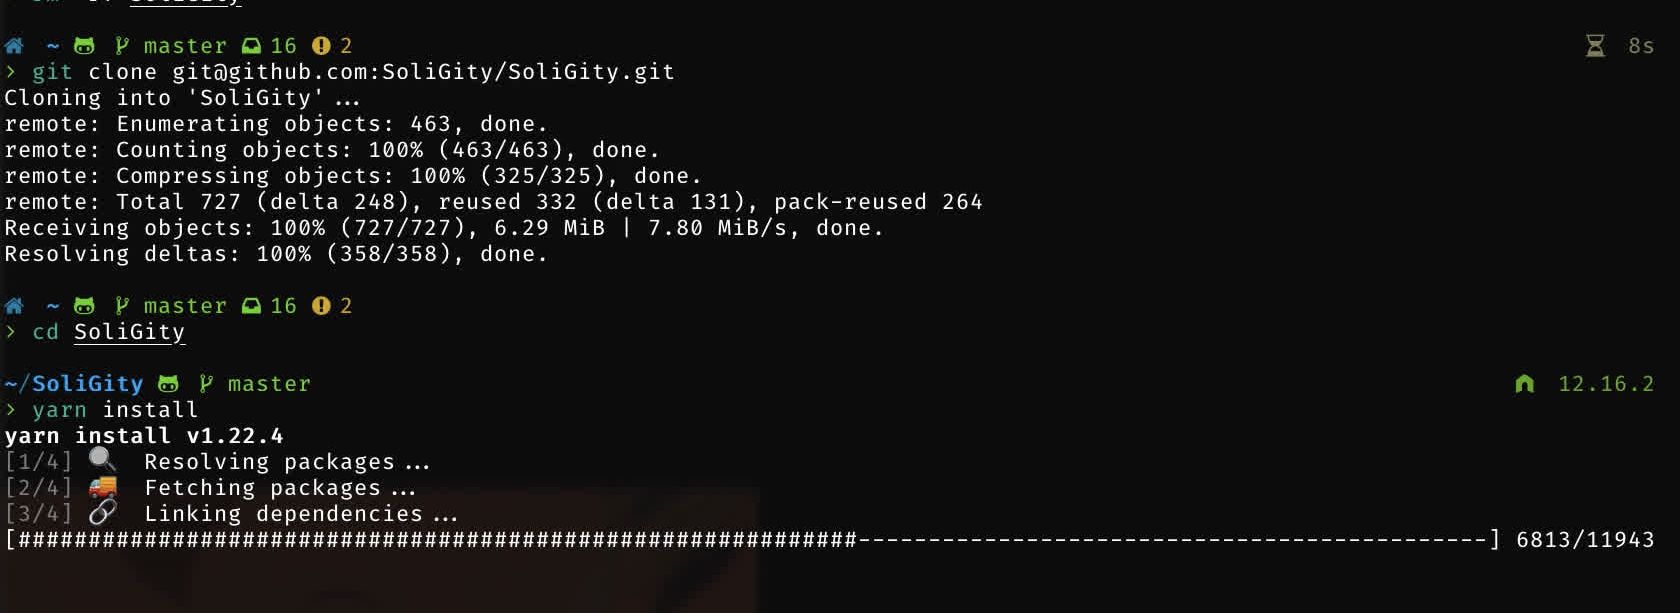
\includegraphics[width=\textwidth]{graphs/01. git_clone}
% 		\end{subfigure}
% 			\begin{subfigure}[b]{\textwidth}
% 				\captionsetup{justification   = raggedright,
%               singlelinecheck = false}
% 			\centering
% 						\caption*{Backend - \texttt{yarn install}}

% 			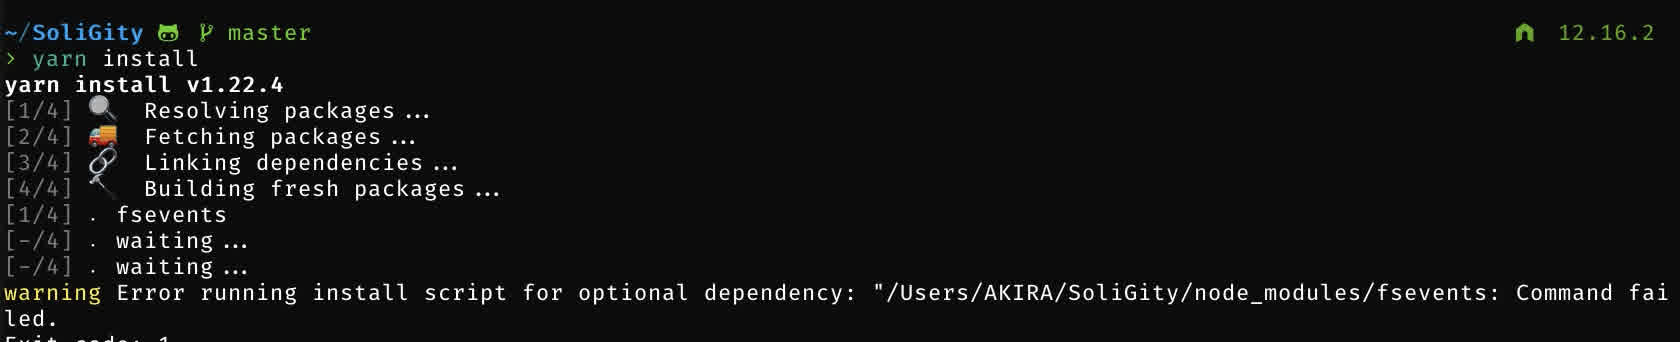
\includegraphics[width=\textwidth]{graphs/02. yarn_install_backend}

% 		\end{subfigure}
% 		\begin{subfigure}[b]{\textwidth}
% 			\captionsetup{justification   = raggedright,
%               singlelinecheck = false}
% 			\centering
% 						\caption*{Backend - user database migrate}

% 			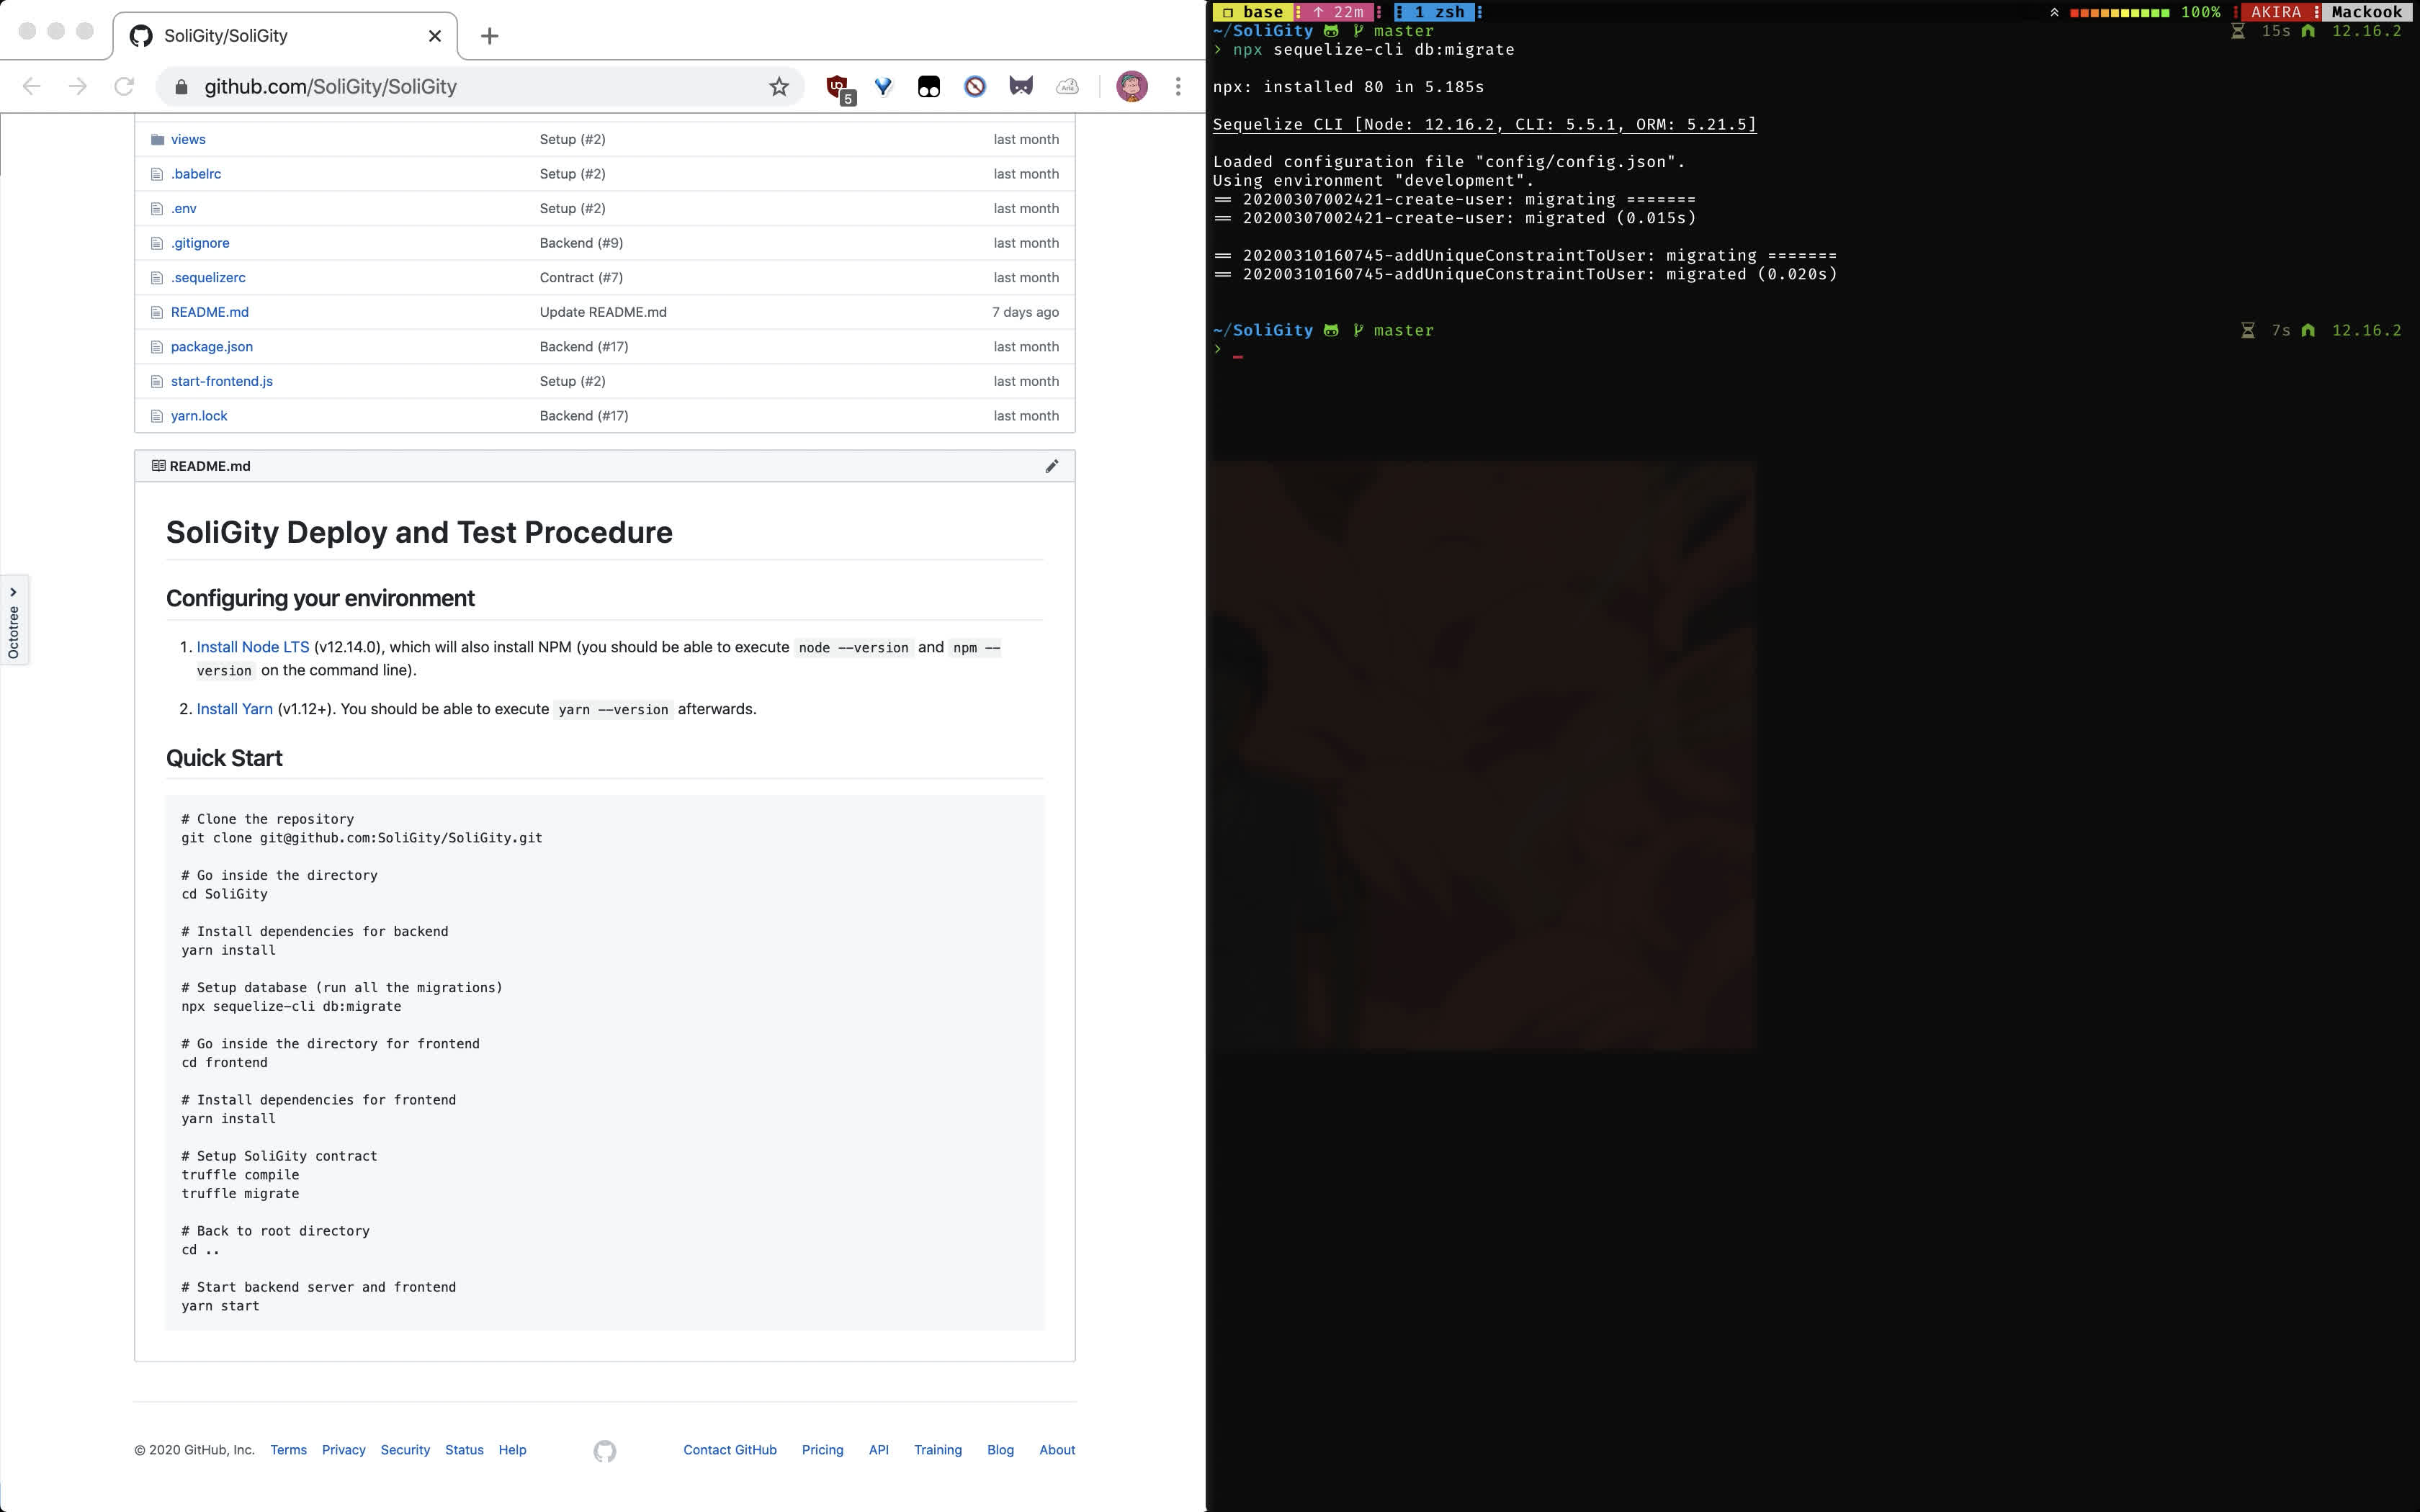
\includegraphics[width=\textwidth]{graphs/03. user_db_migrate}
% 		\end{subfigure}

% 	\end{minipage}
% \end{figure}

\begin{figure}[H]
	\begin{minipage}[t]{0.4\linewidth}
		\begin{lstlisting}[language=bash]
# Clone the repository
git clone git@github.com:SoliGity/SoliGity.git

# Go inside the directory
cd SoliGity

# Install dependencies for backend
yarn install

# Setup database (run all the migrations)
npx sequelize-cli db:migrate

# Go inside the directory for frontend
cd frontend

# Install dependencies for frontend
yarn install

# Setup SoliGity contract
truffle compile
truffle migrate

# Back to root directory
cd ..
# Start backend server and frontend
yarn start
				\end{lstlisting}
				
				   	\begin{subfigure}[t]{1.2\textwidth}
	\captionsetup{justification   = raggedright,
              singlelinecheck = false}
		\centering
				\caption*{\textbf{Setup Output} - \texttt{truffle migrate}}
		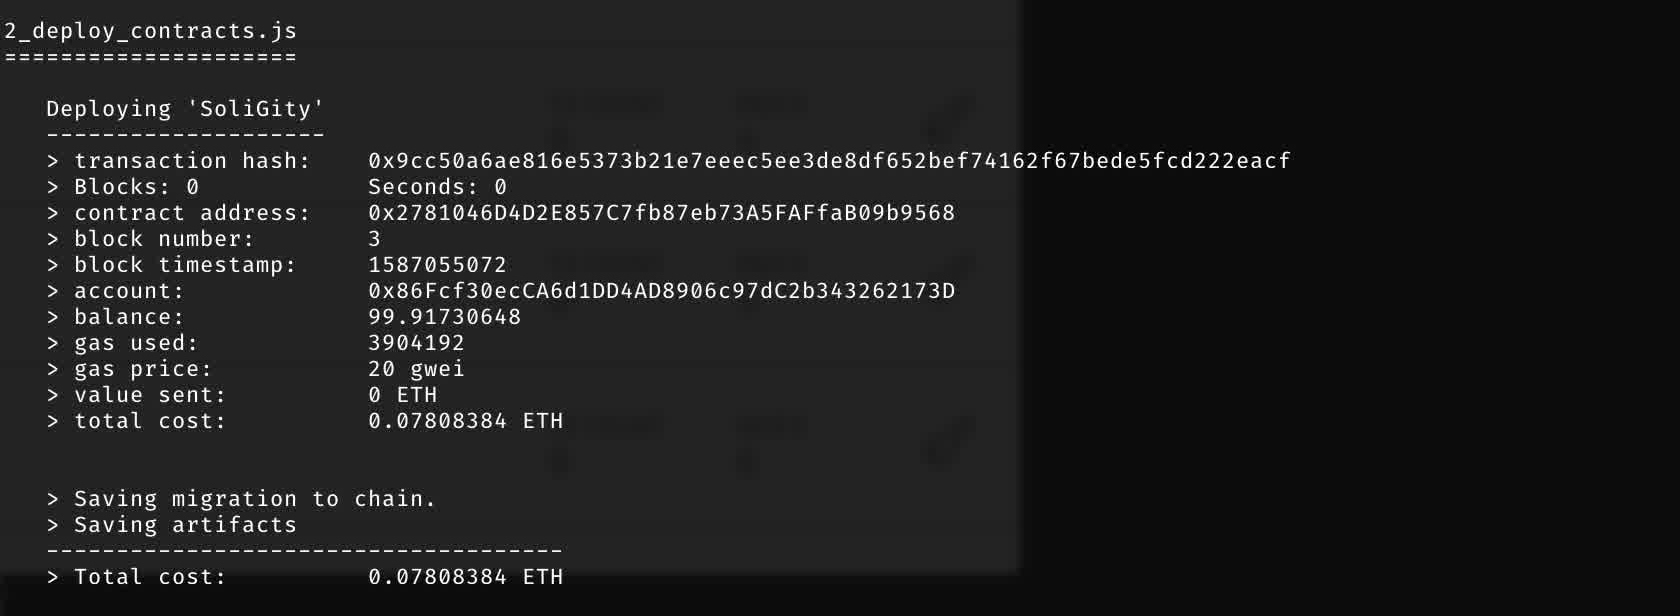
\includegraphics[width=\textwidth]{graphs/07. truffle_migrate}
	\end{subfigure}
	\end{minipage}\hfill
	\begin{minipage}[t]{0.5\linewidth}
		% \begin{figure}[H]
% 				\begin{subfigure}[b]{\textwidth}
% 			\captionsetup{justification   = raggedright,
%               singlelinecheck = false}
% 			\centering
% 						\caption*{\textbf{Setup Output - }\texttt{git clone}}
% 			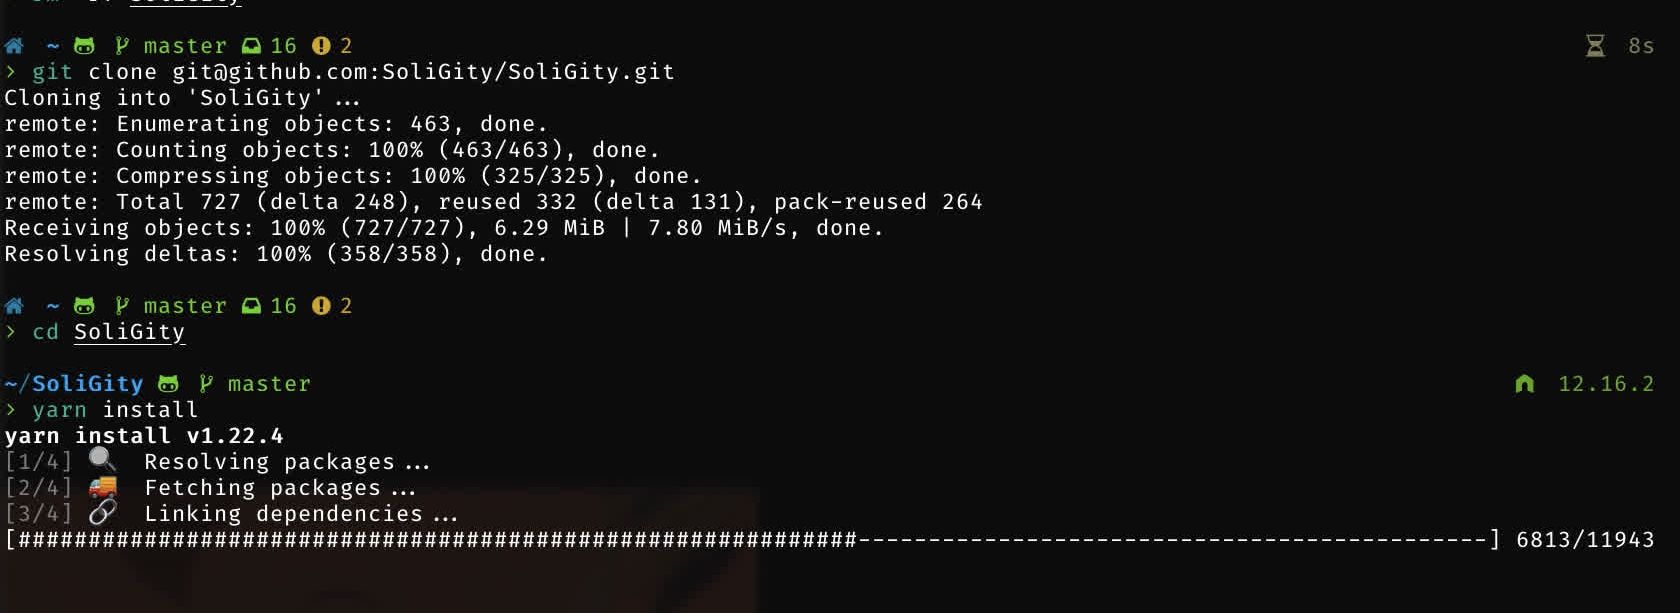
\includegraphics[width=\textwidth]{graphs/01. git_clone}
% 		\end{subfigure}
			\begin{subfigure}[b]{\textwidth}
				\captionsetup{justification   = raggedright,
              singlelinecheck = false}
			\centering
						\caption*{Backend - \texttt{yarn install}}

			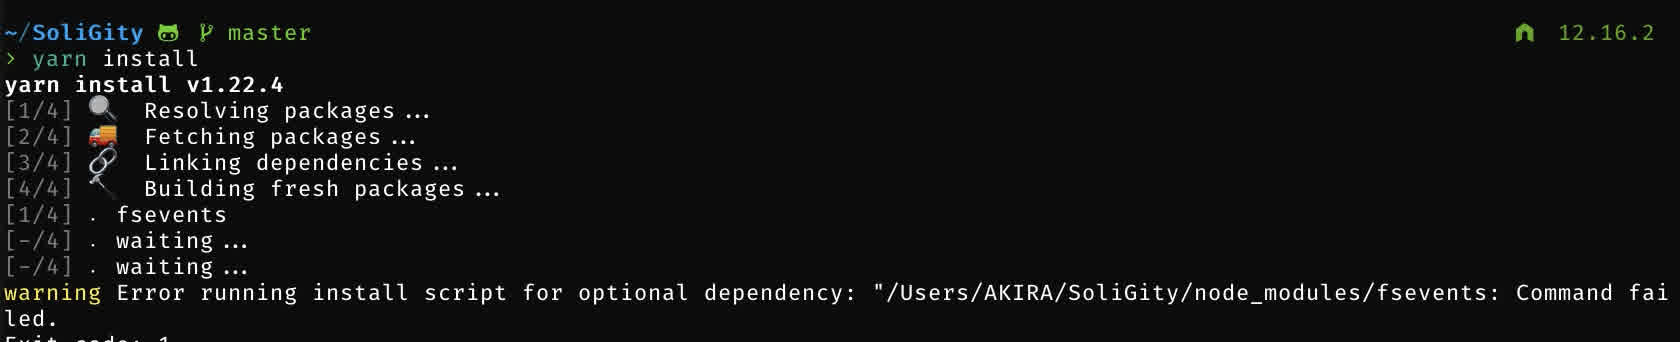
\includegraphics[width=\textwidth]{graphs/02. yarn_install_backend}

		\end{subfigure}
% 		\begin{subfigure}[b]{\textwidth}
% 			\captionsetup{justification   = raggedright,
%               singlelinecheck = false}
% 			\centering
% 						\caption*{Backend - user database migrate}

% 			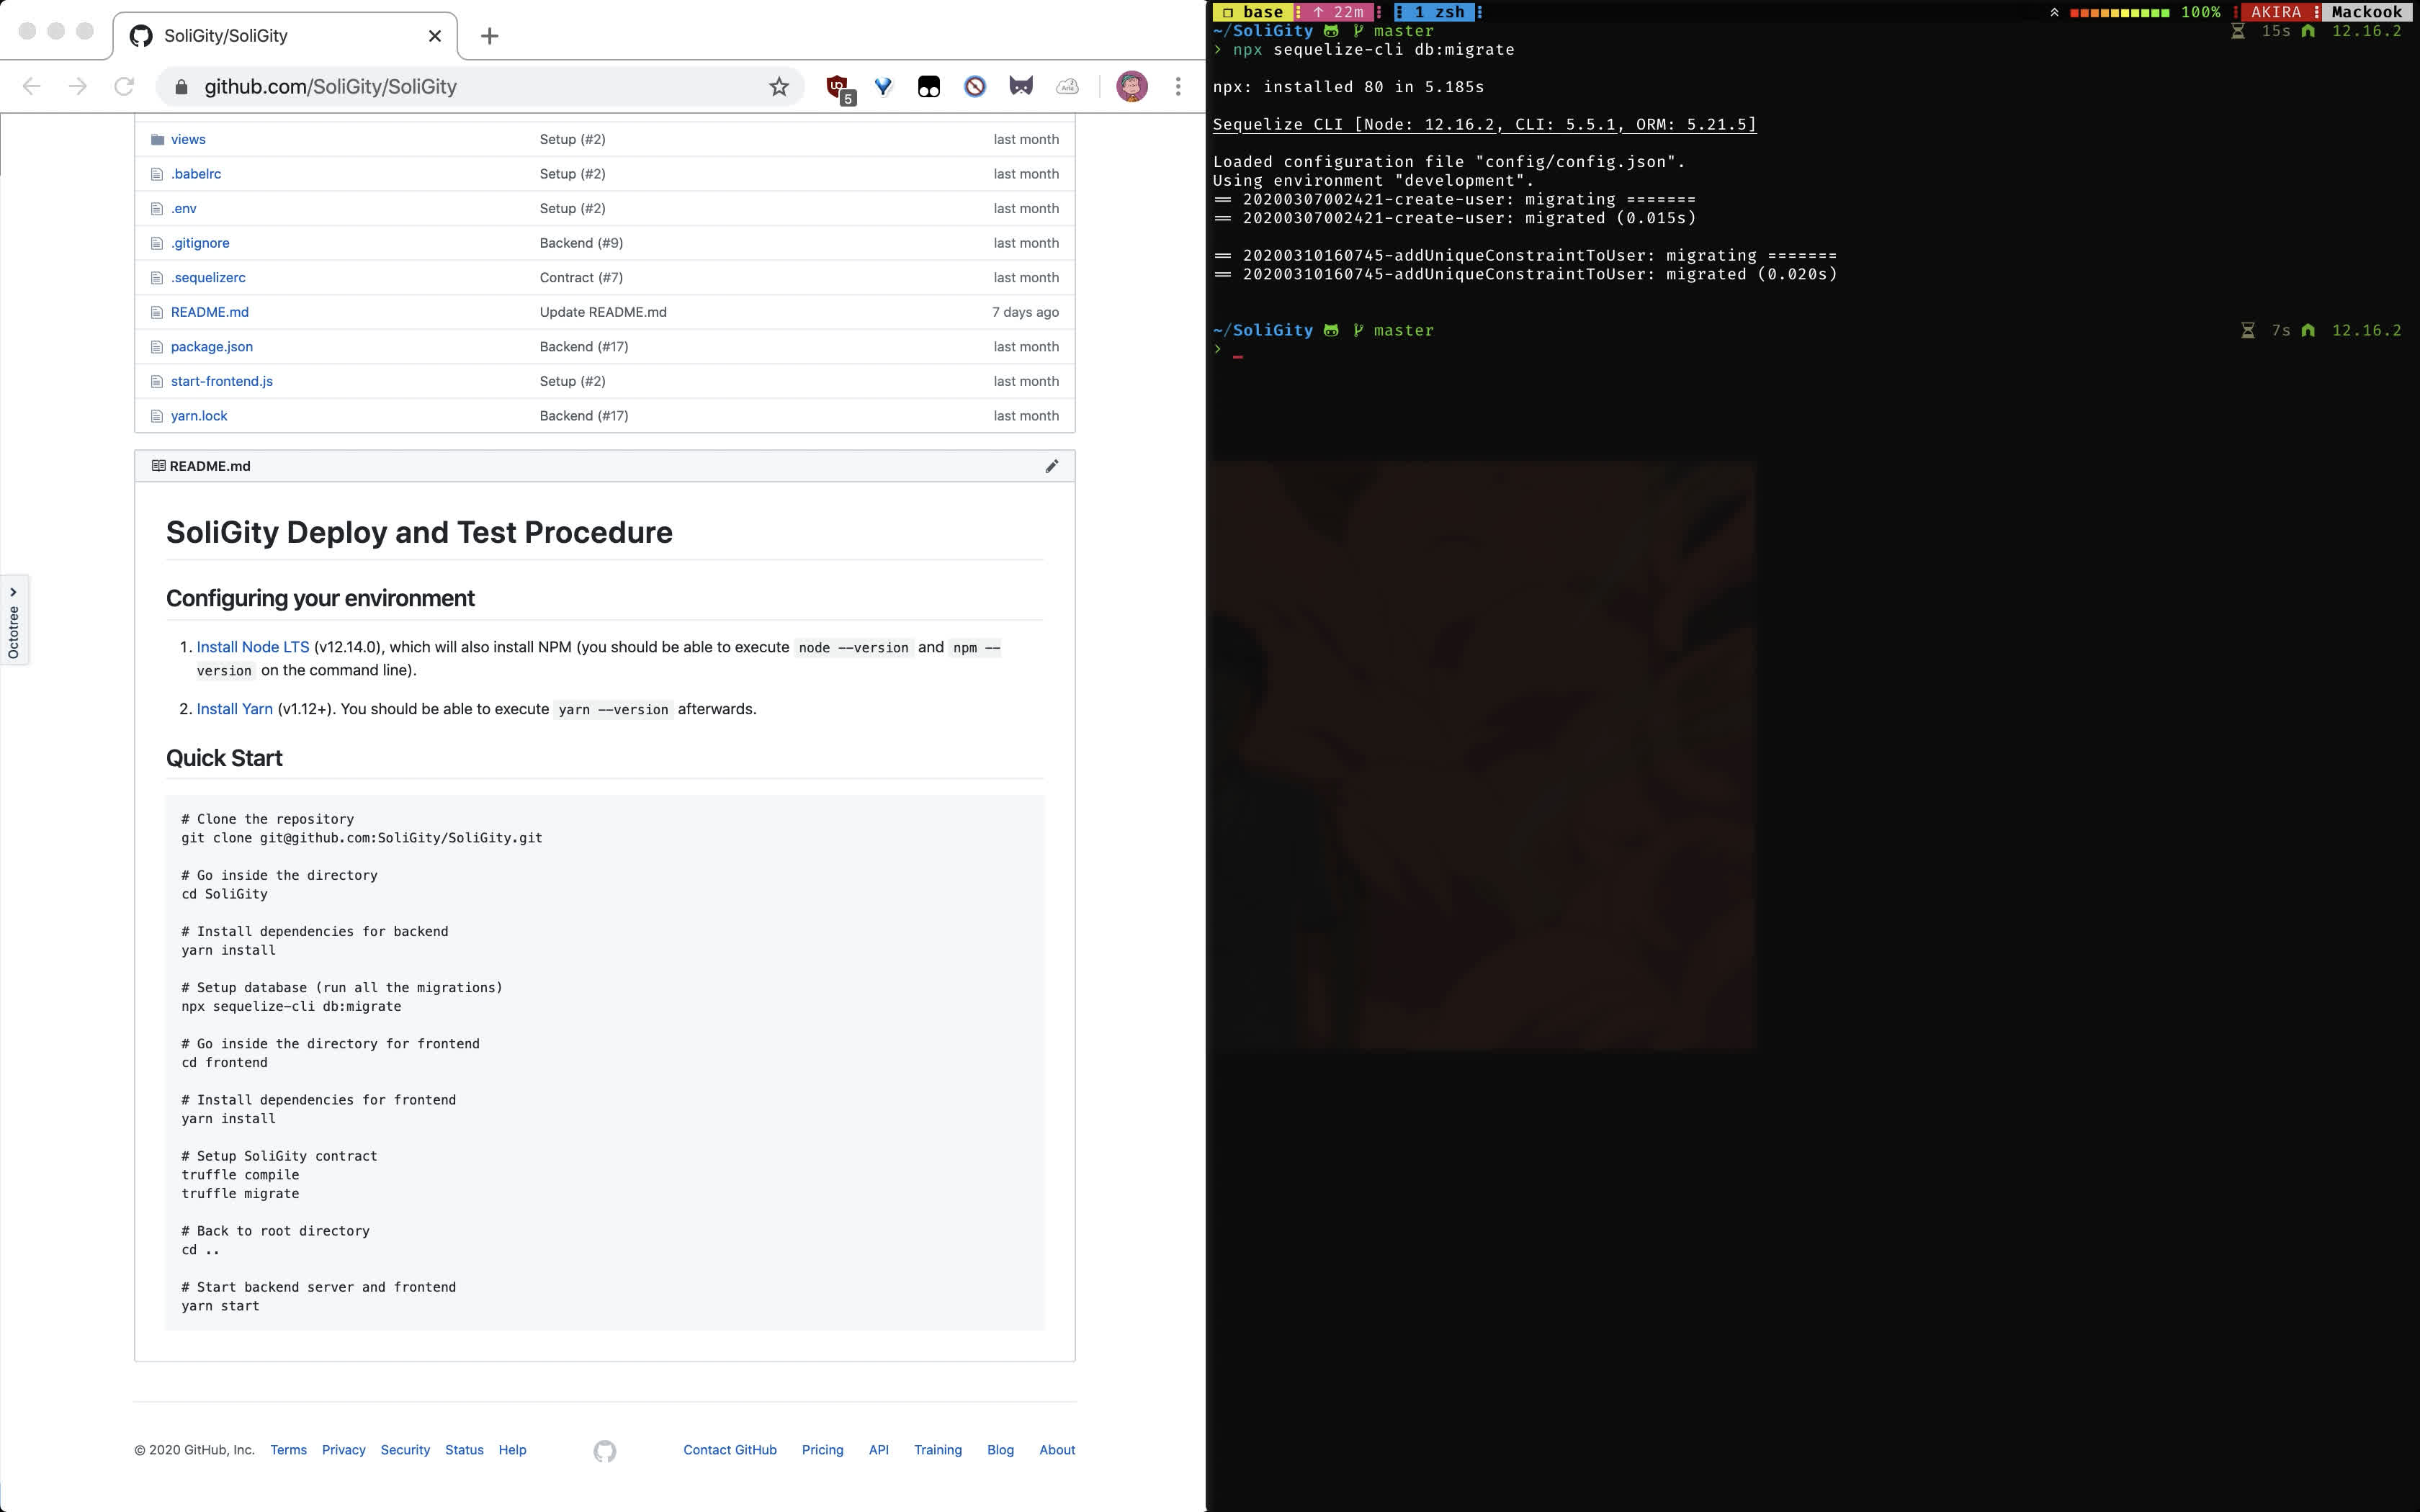
\includegraphics[width=\textwidth]{graphs/03. user_db_migrate}
% 		\end{subfigure}

					\begin{subfigure}[b]{\textwidth}
				\captionsetup{justification   = raggedright,
              singlelinecheck = false}
			\centering
						\caption*{Frontend - \texttt{yarn install}}

			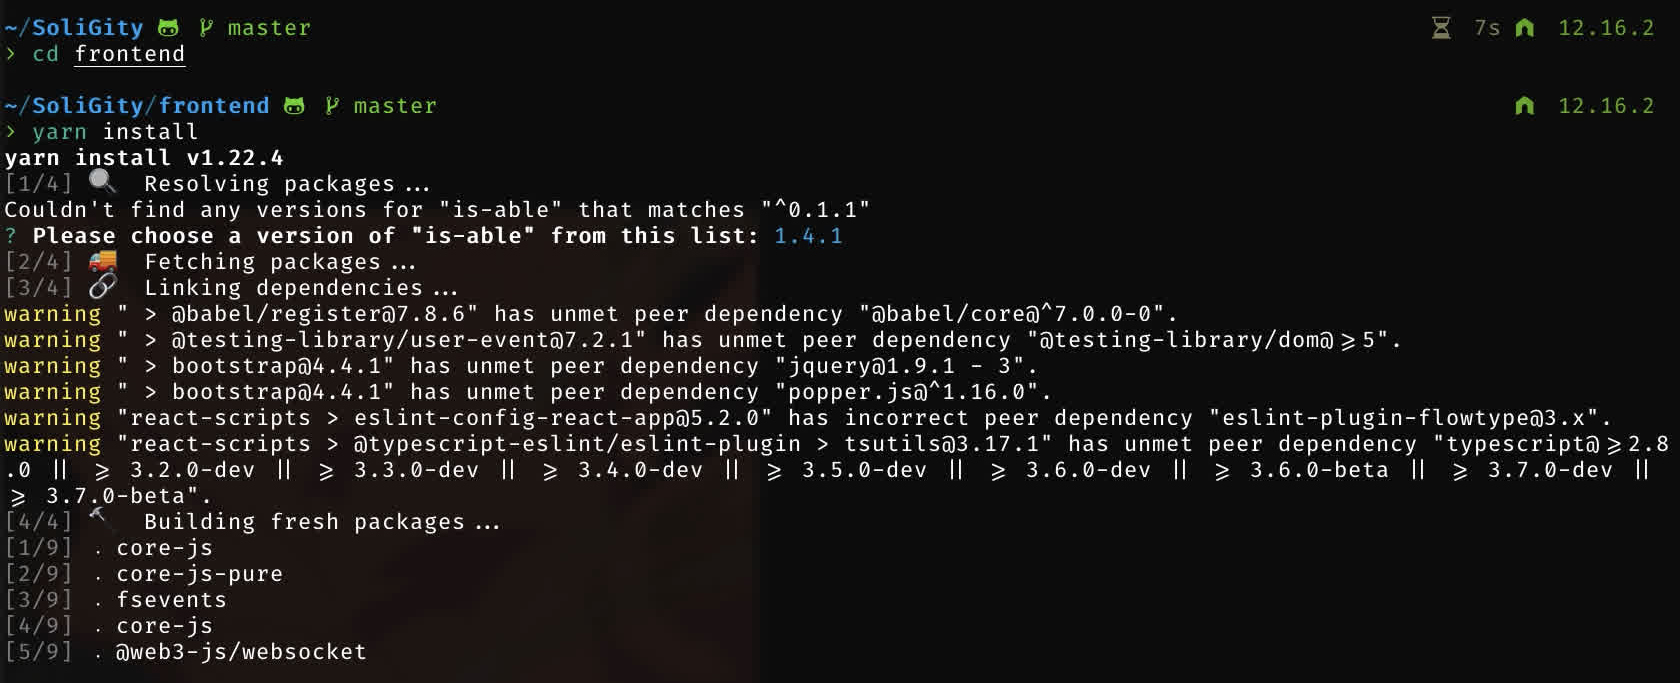
\includegraphics[width=\textwidth]{graphs/04. yarn_install_frontend}
		\end{subfigure}
		\centering
		\begin{subfigure}[b]{\textwidth}
			\captionsetup{justification   = raggedright,
              singlelinecheck = false}
		\centering
				\caption*{\textbf{Setup Output} - \texttt{truffle Compile}}
		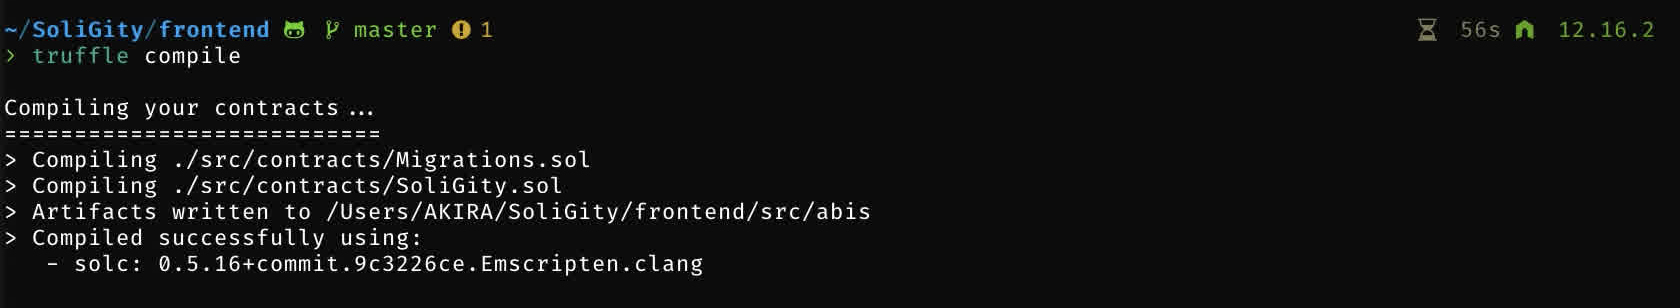
\includegraphics[width=\textwidth]{graphs/05. truffle_compile}
		\end{subfigure}
			\begin{subfigure}[b]{\textwidth}
	\captionsetup{justification   = raggedright,
              singlelinecheck = false}
		\centering
				\caption*{\textbf{Ganache Setup}}
		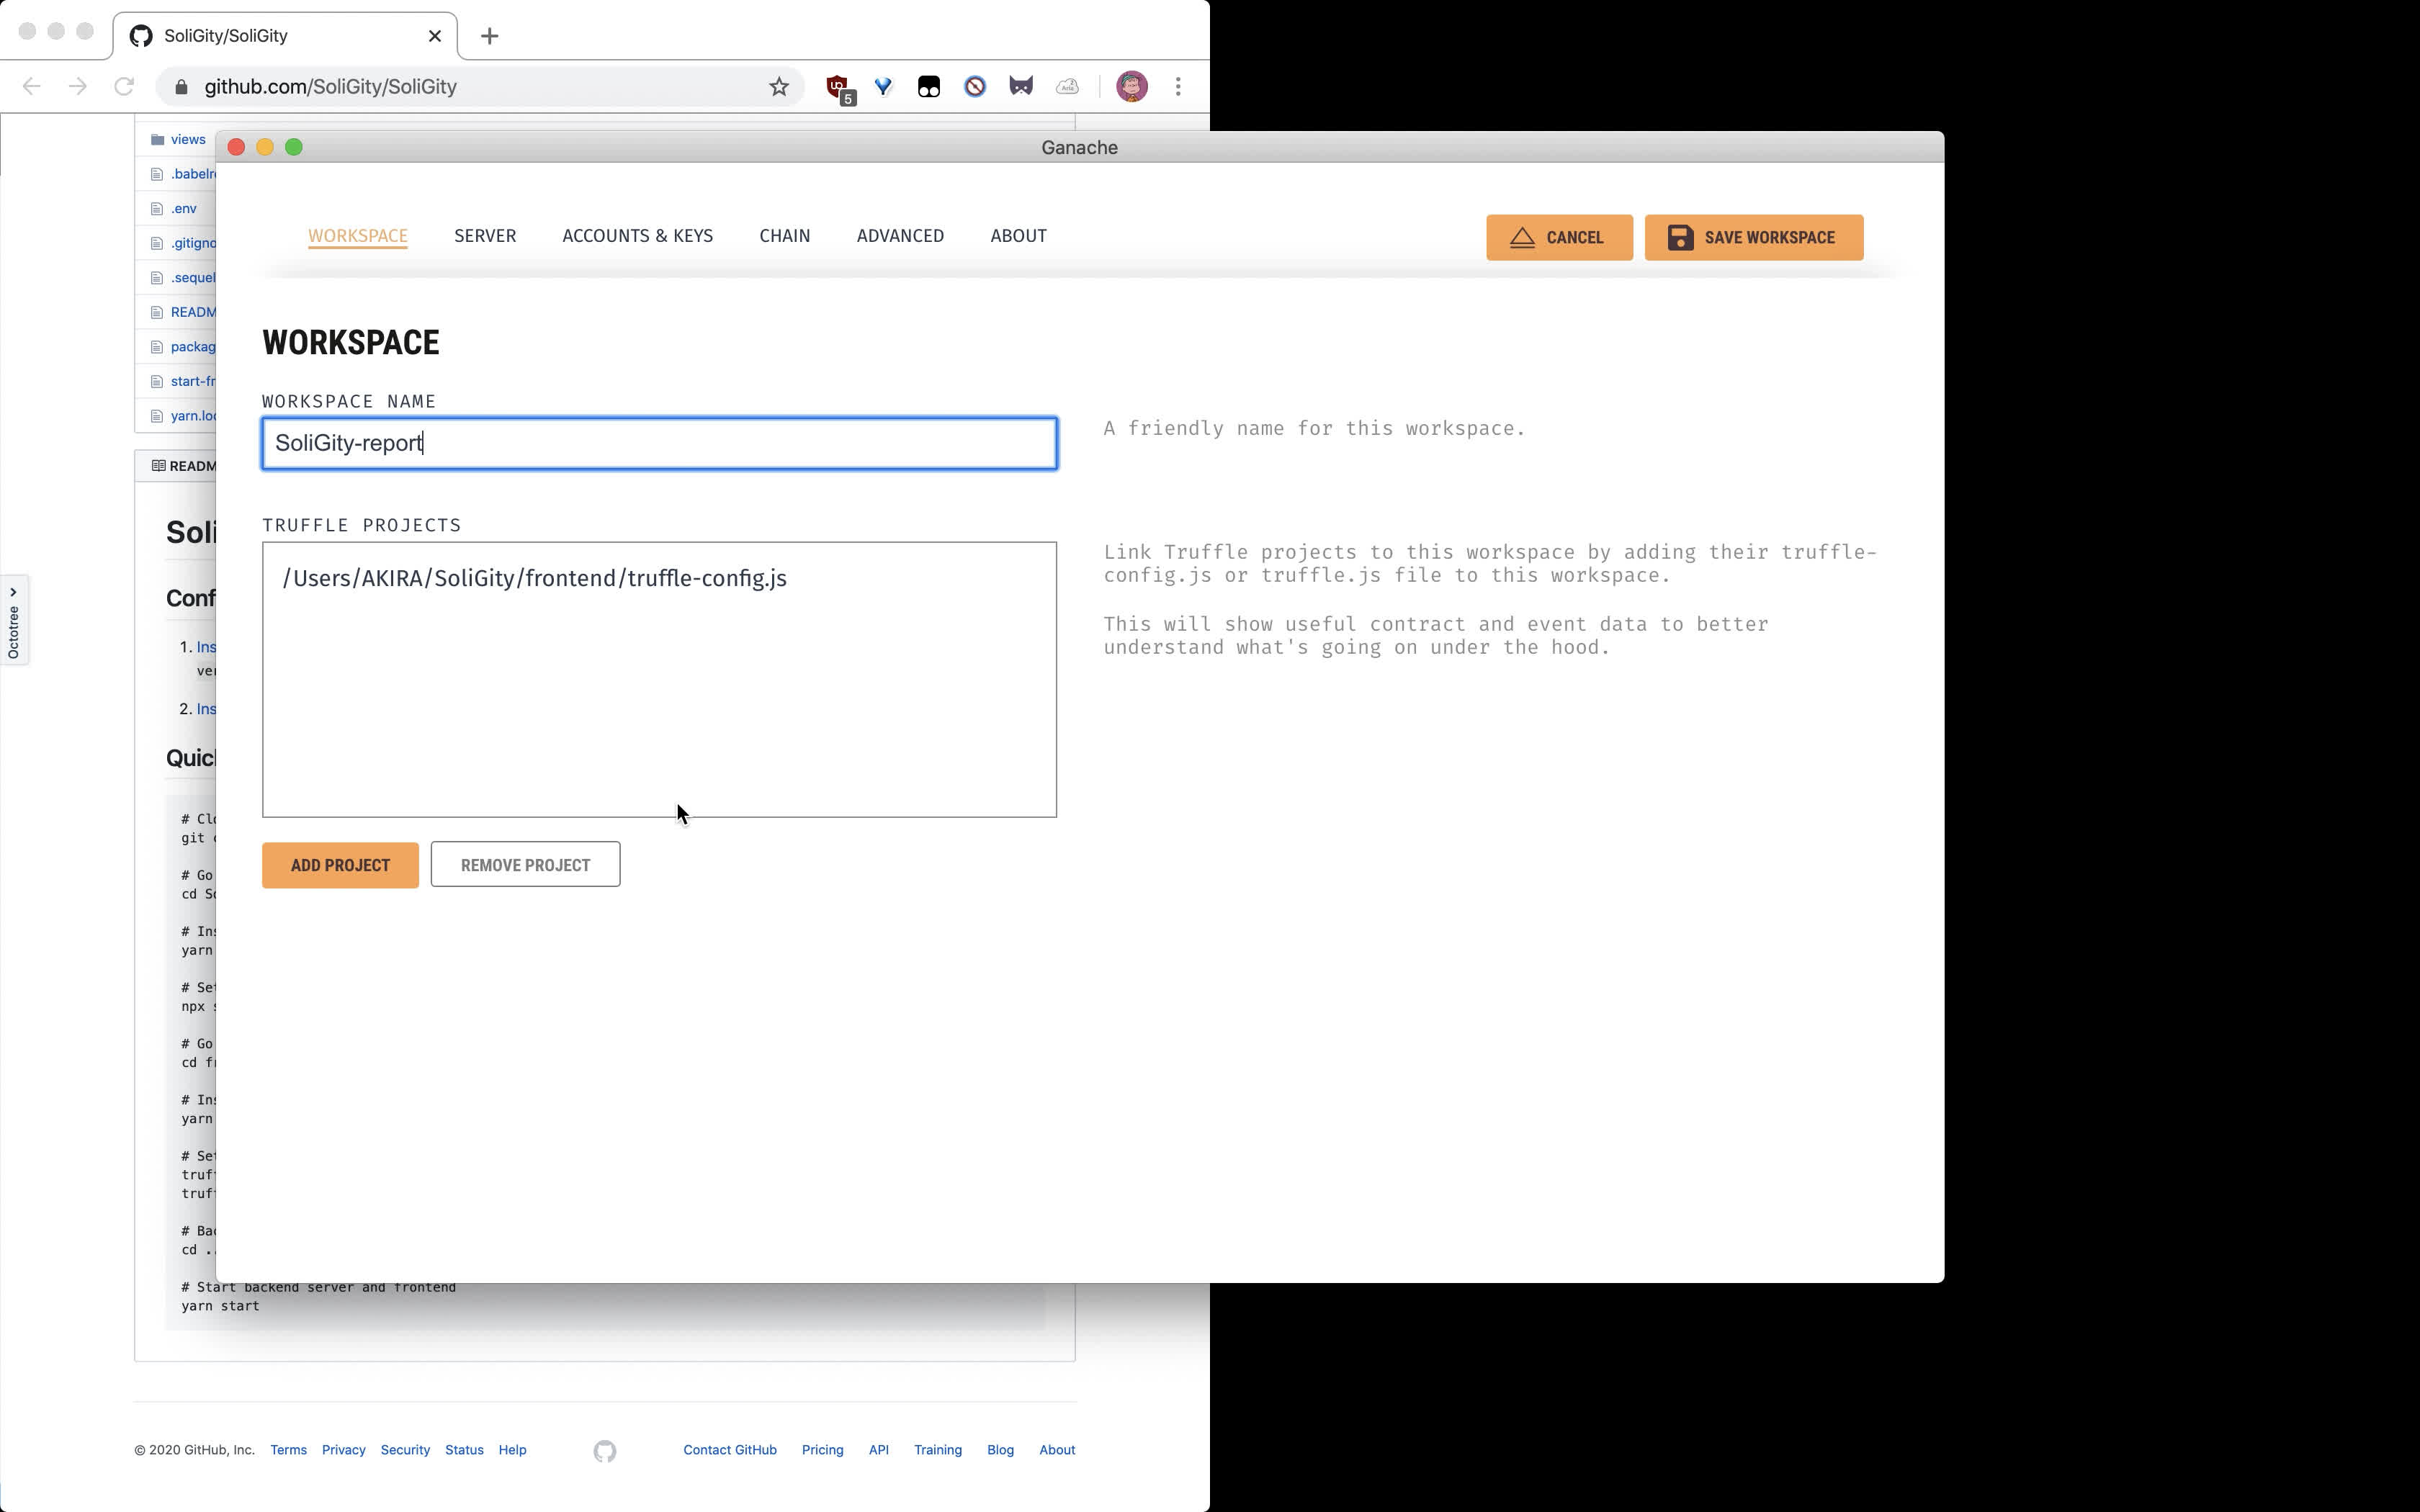
\includegraphics[width=\textwidth]{graphs/06. ganache_setup}
		\end{subfigure}

% 	\begin{subfigure}[t]{\textwidth}
% 	\captionsetup{justification   = raggedright,
%               singlelinecheck = false}
% 		\centering
% 				\caption*{\textbf{Setup Output} - \texttt{truffle migrate}}
% 		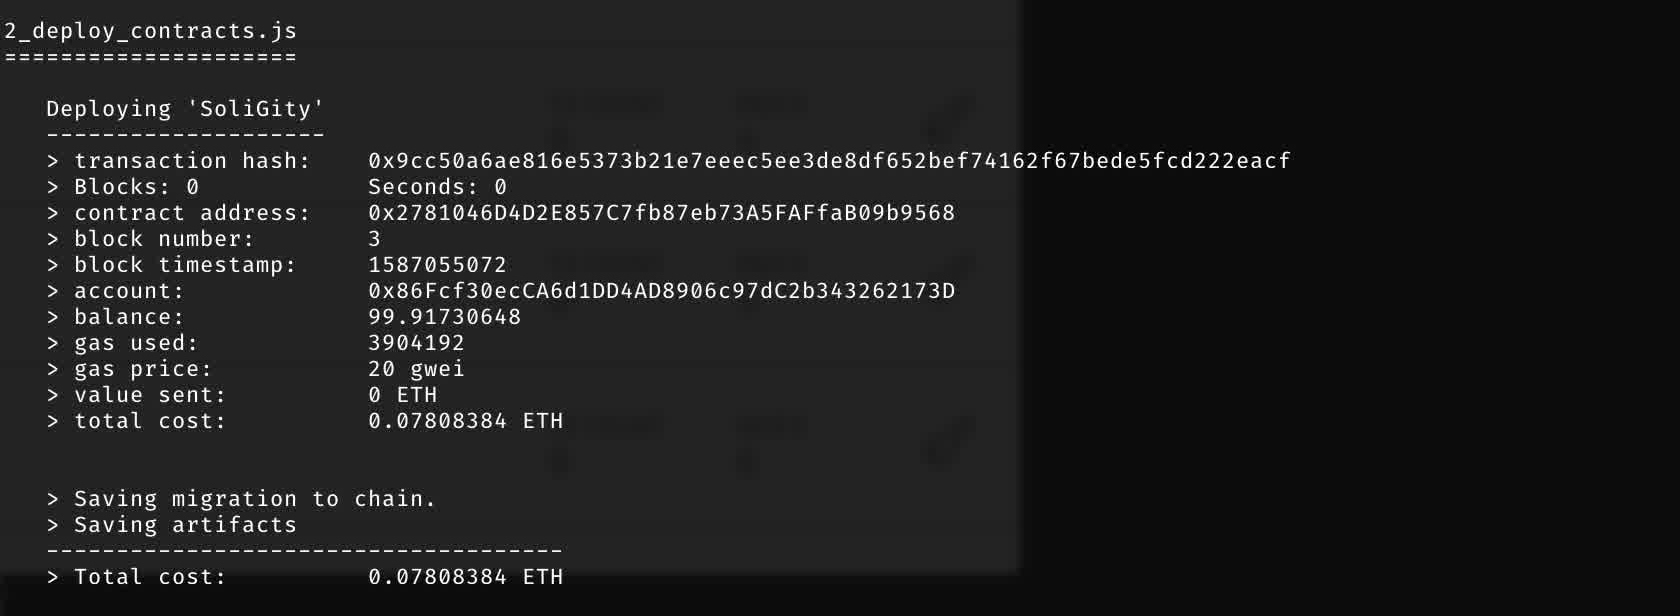
\includegraphics[width=\textwidth]{graphs/07. truffle_migrate}
% 	\end{subfigure}
	\begin{subfigure}[t]{\textwidth}
	\captionsetup{justification   = raggedright,
              singlelinecheck = false}
		\centering
				\caption*{\textbf{Deployed Contract}}
		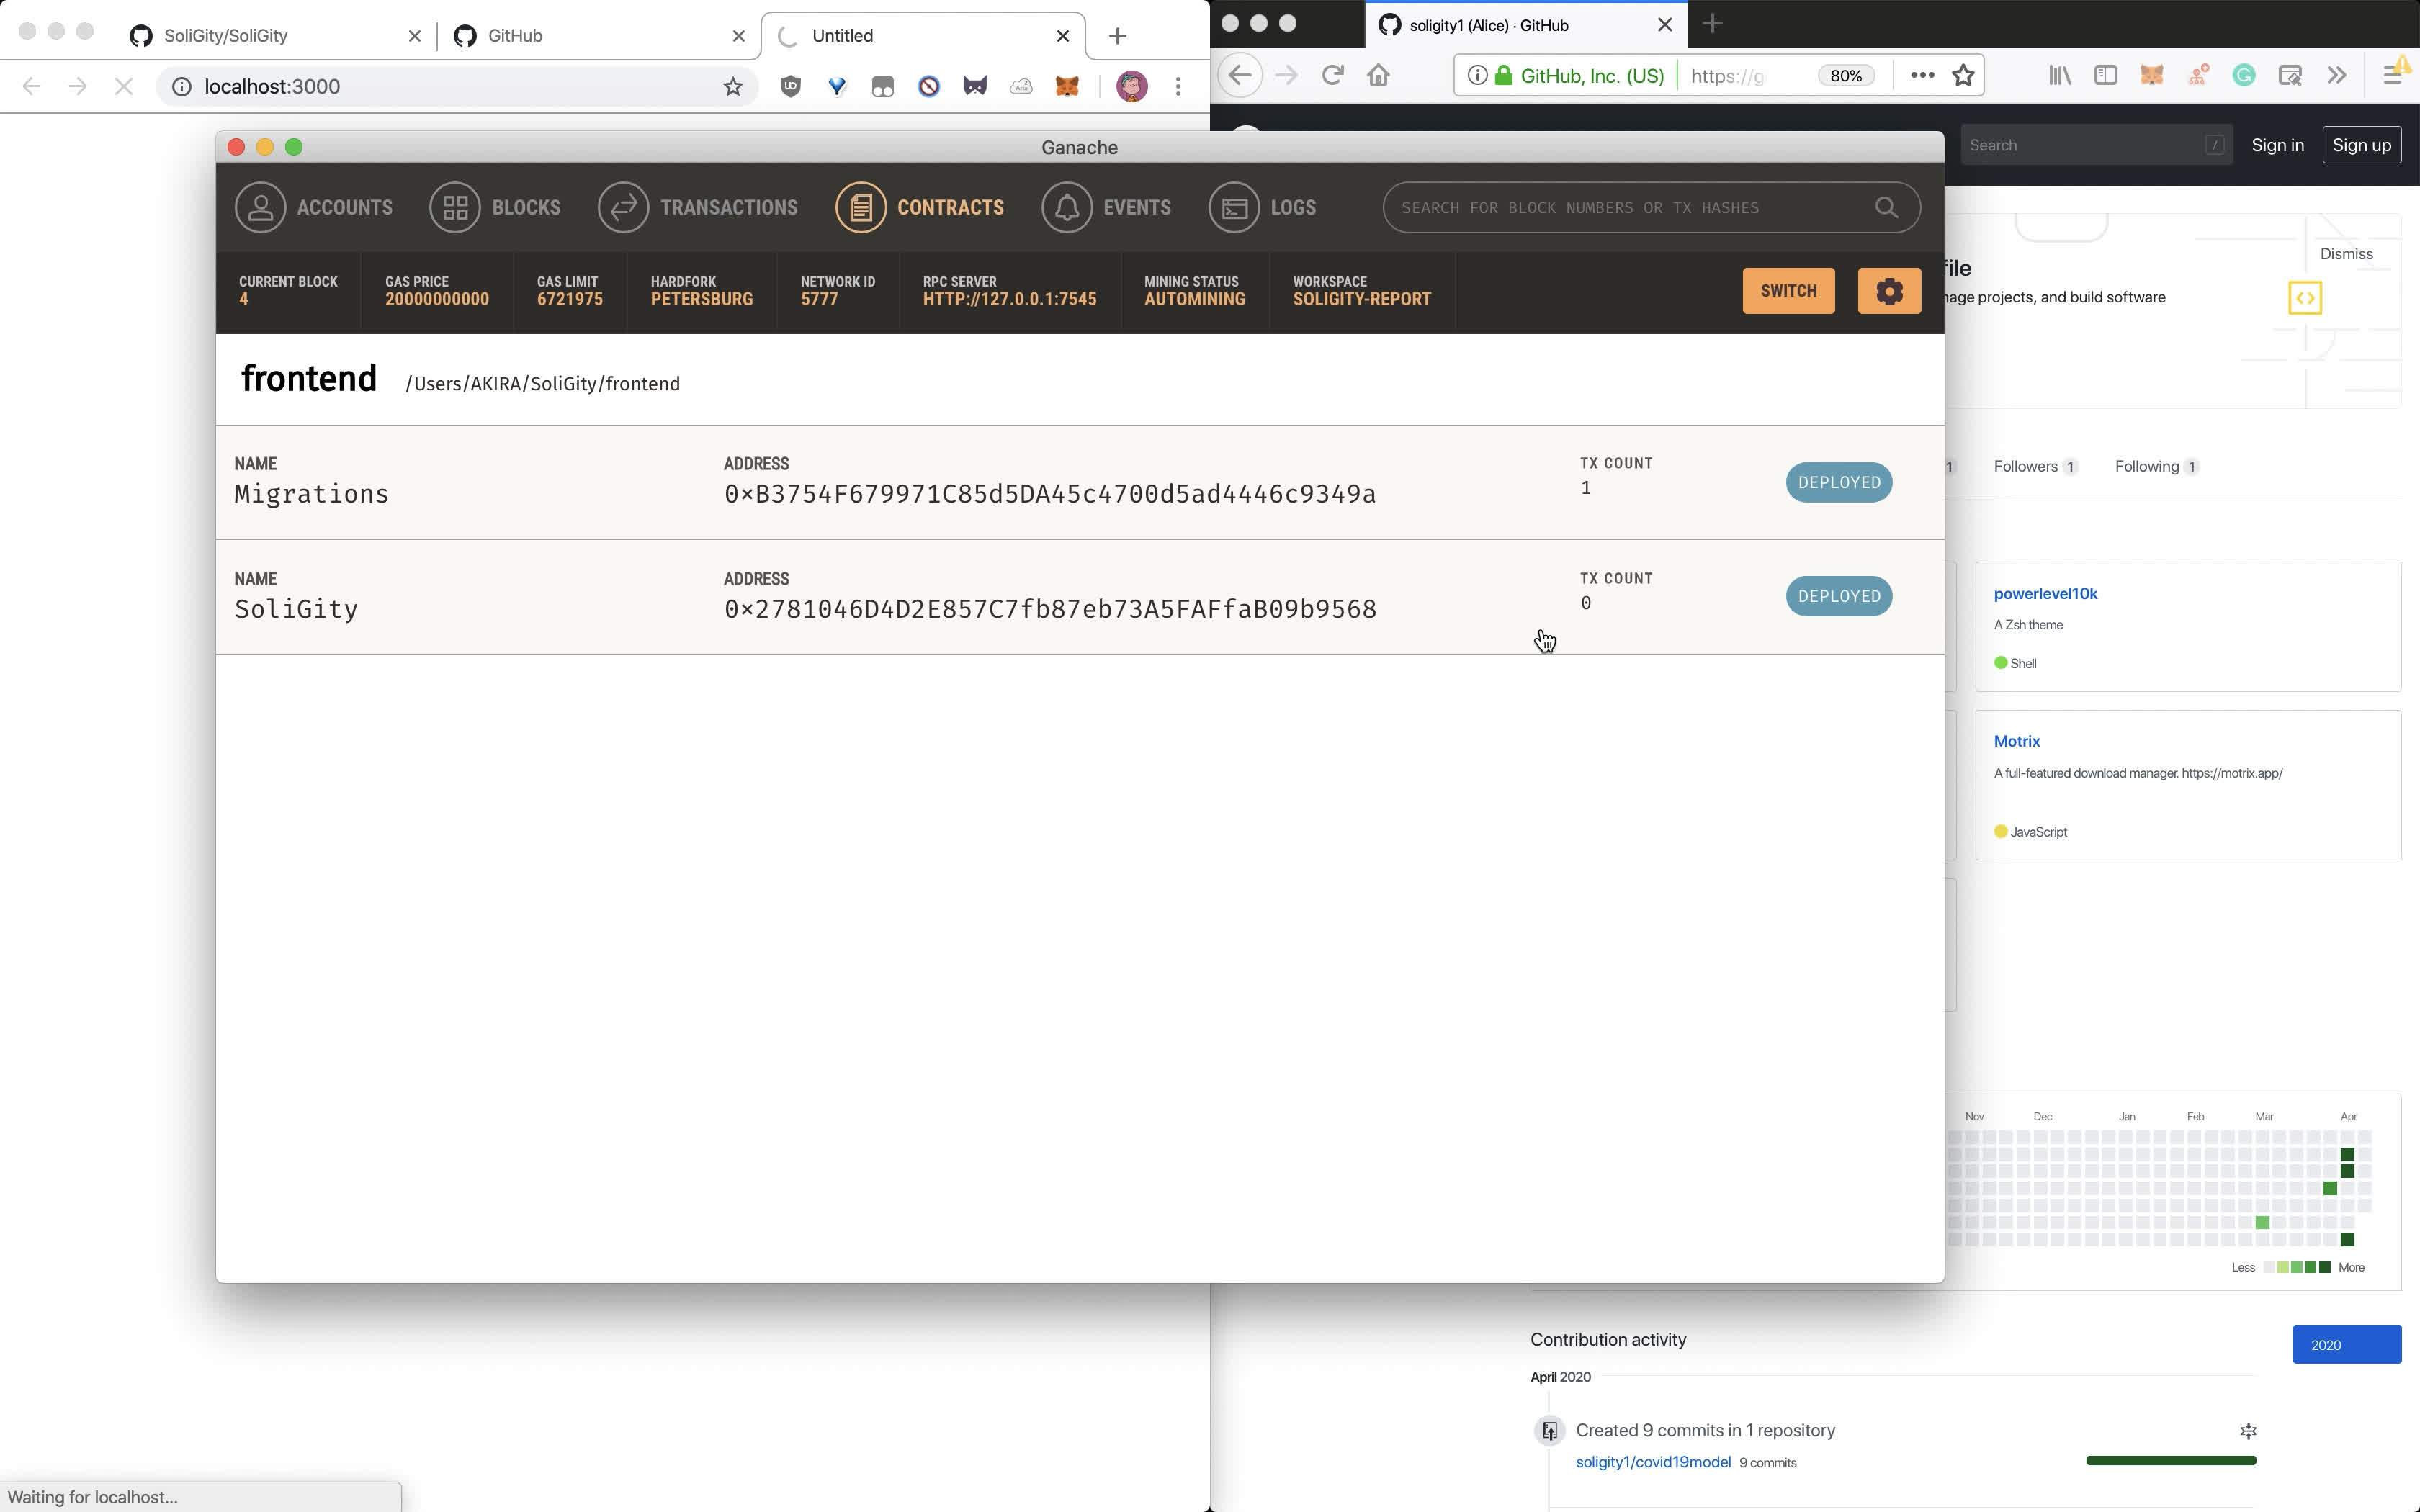
\includegraphics[width=\textwidth]{graphs/08. ganache_deployed_contract}
	\end{subfigure}

	\end{minipage}
	\caption{Environment Setup}
	\label{fig:setup0}
\end{figure}

% \begin{figure}[H]
%     \centering
%   	\begin{subfigure}[t]{0.45\textwidth}
% 	\captionsetup{justification   = raggedright,
%               singlelinecheck = false}
% 		\centering
% 				\caption*{\textbf{Setup Output} - \texttt{truffle migrate}}
% 		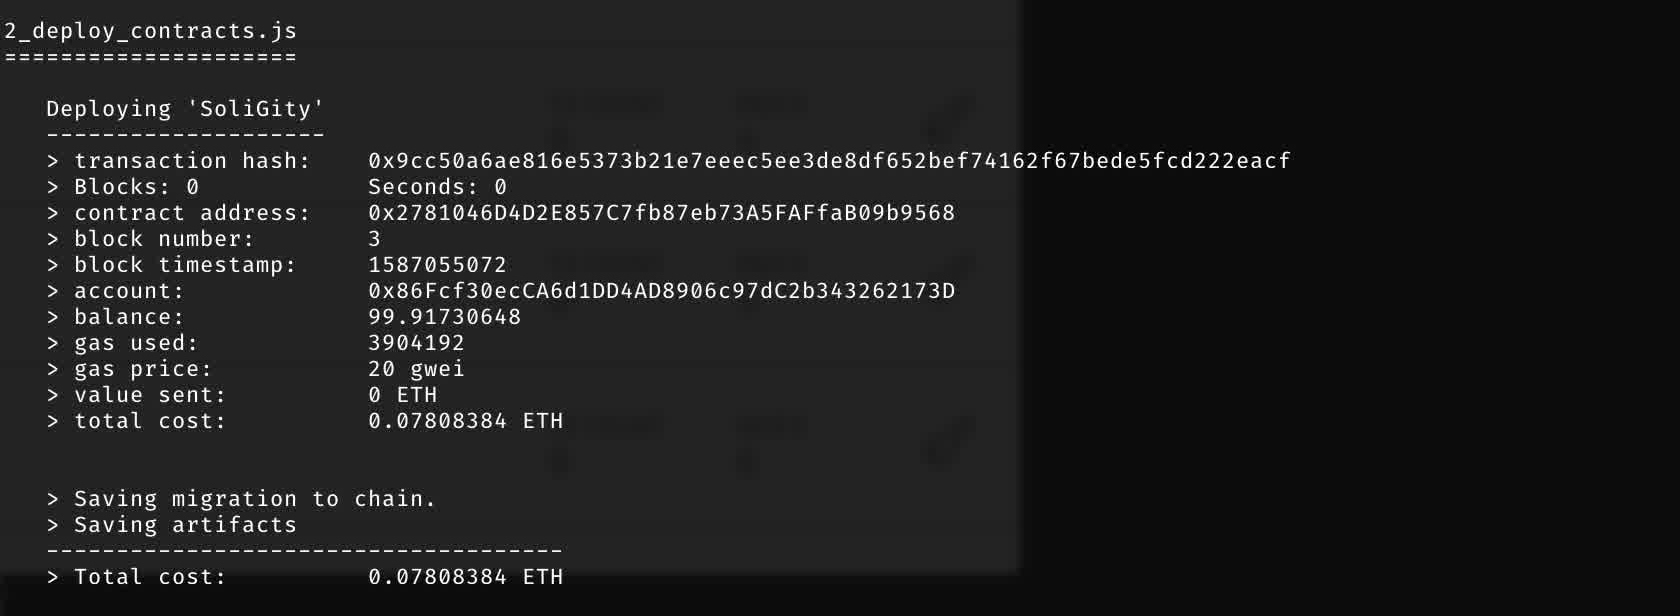
\includegraphics[width=\textwidth]{graphs/07. truffle_migrate}
% 	\end{subfigure}
% 	\hfill
% 	\begin{subfigure}[t]{0.45\textwidth}
% 	\captionsetup{justification   = raggedright,
%               singlelinecheck = false}
% 		\centering
% 				\caption*{\textbf{Deployed Contract}}
% 		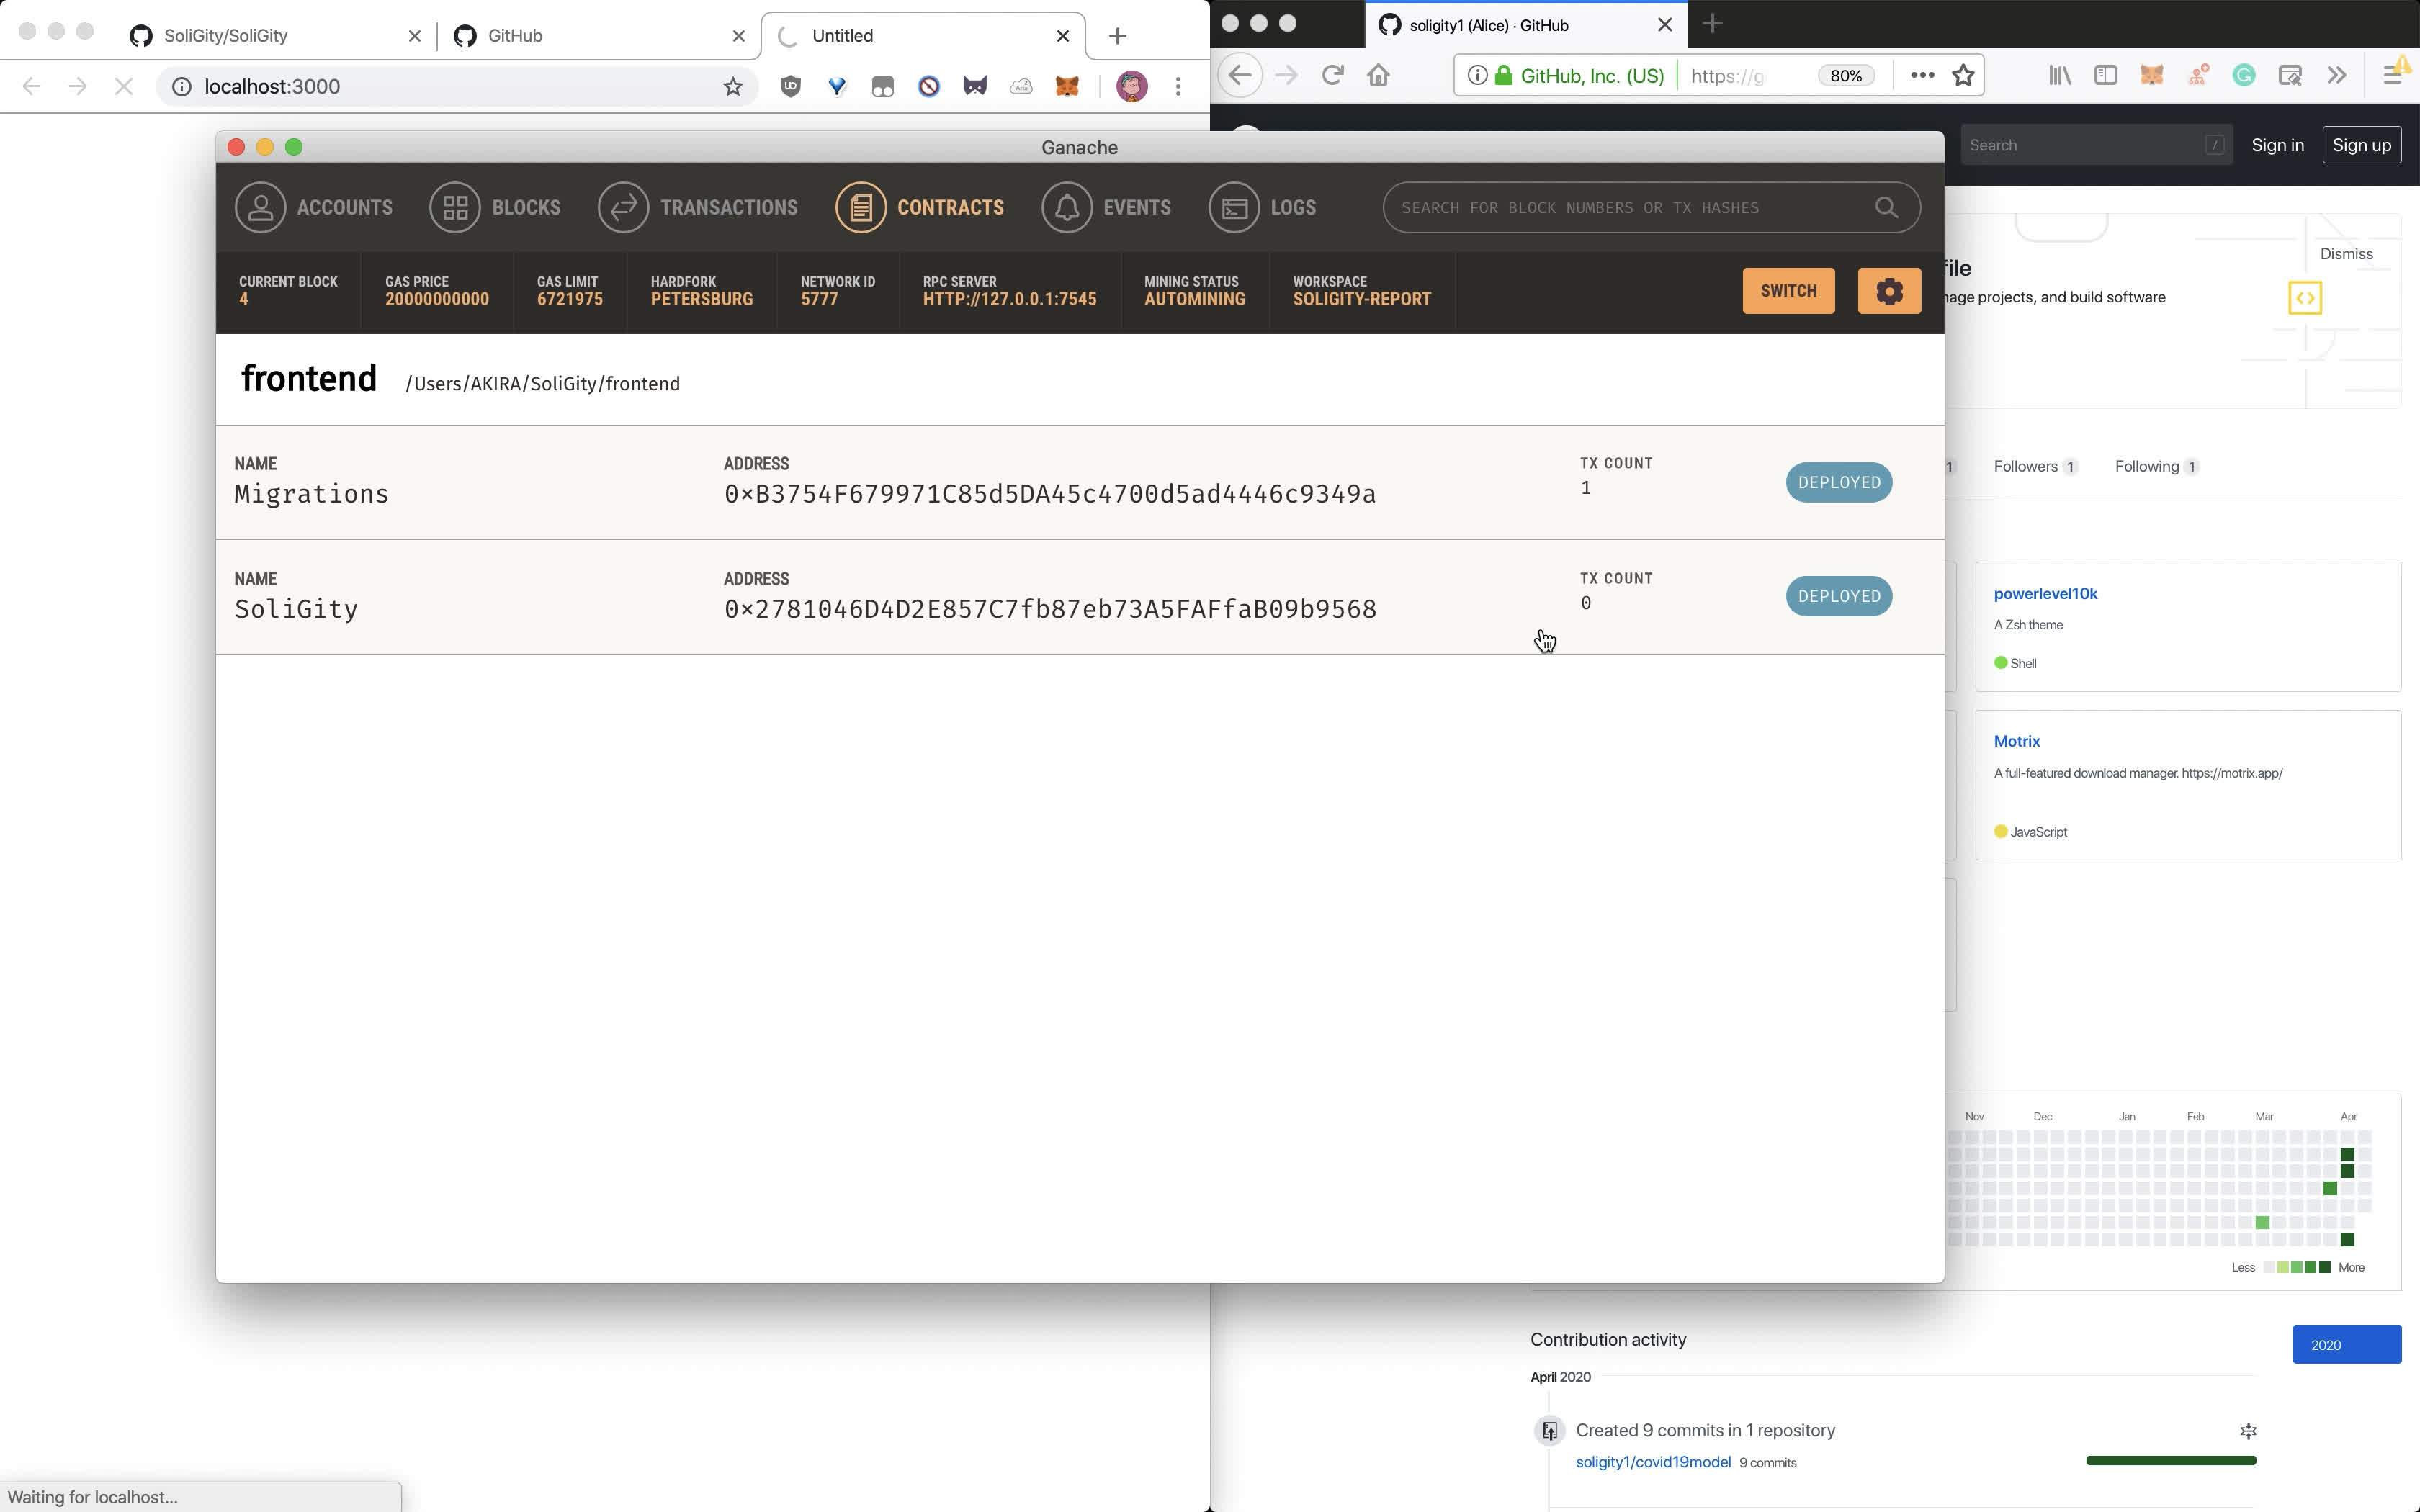
\includegraphics[width=\textwidth]{graphs/08. ganache_deployed_contract}
% 	\end{subfigure}
%     % \caption{Caption}
%     % \label{fig:my_label}
% \end{figure}
% \begin{figure}[H]

% 	\centering
% 	\begin{subfigure}[t]{.45\textwidth}
% 	\captionsetup{justification   = raggedright,
%               singlelinecheck = false}
% 		\centering
% 				\caption*{\textbf{Setup Output} - \texttt{truffle Compile}}
% 		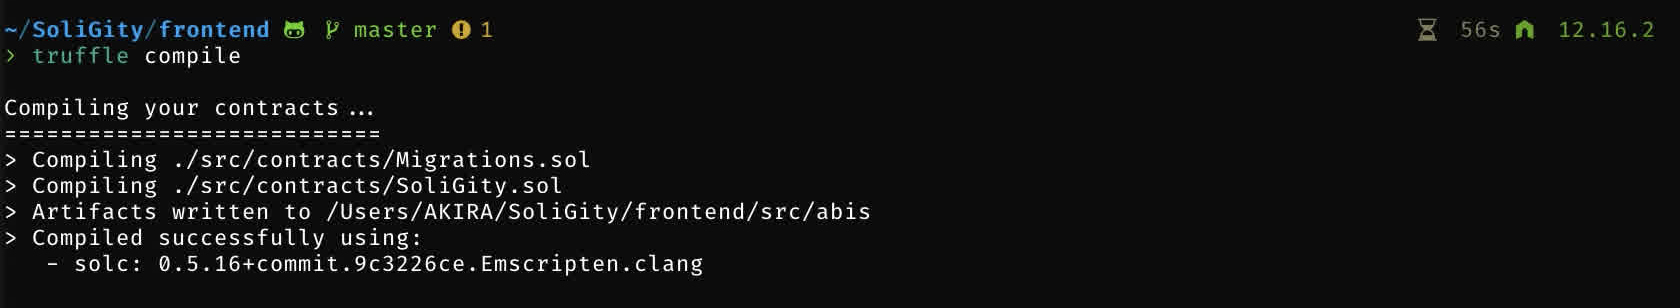
\includegraphics[width=\textwidth]{graphs/05. truffle_compile.jpg}
% 	\end{subfigure}
% 	\begin{subfigure}[t]{.45\textwidth}
% 	\captionsetup{justification   = raggedright,
%               singlelinecheck = false}
% 		\centering
% 				\caption*{\textbf{Ganache Setup}}
% 		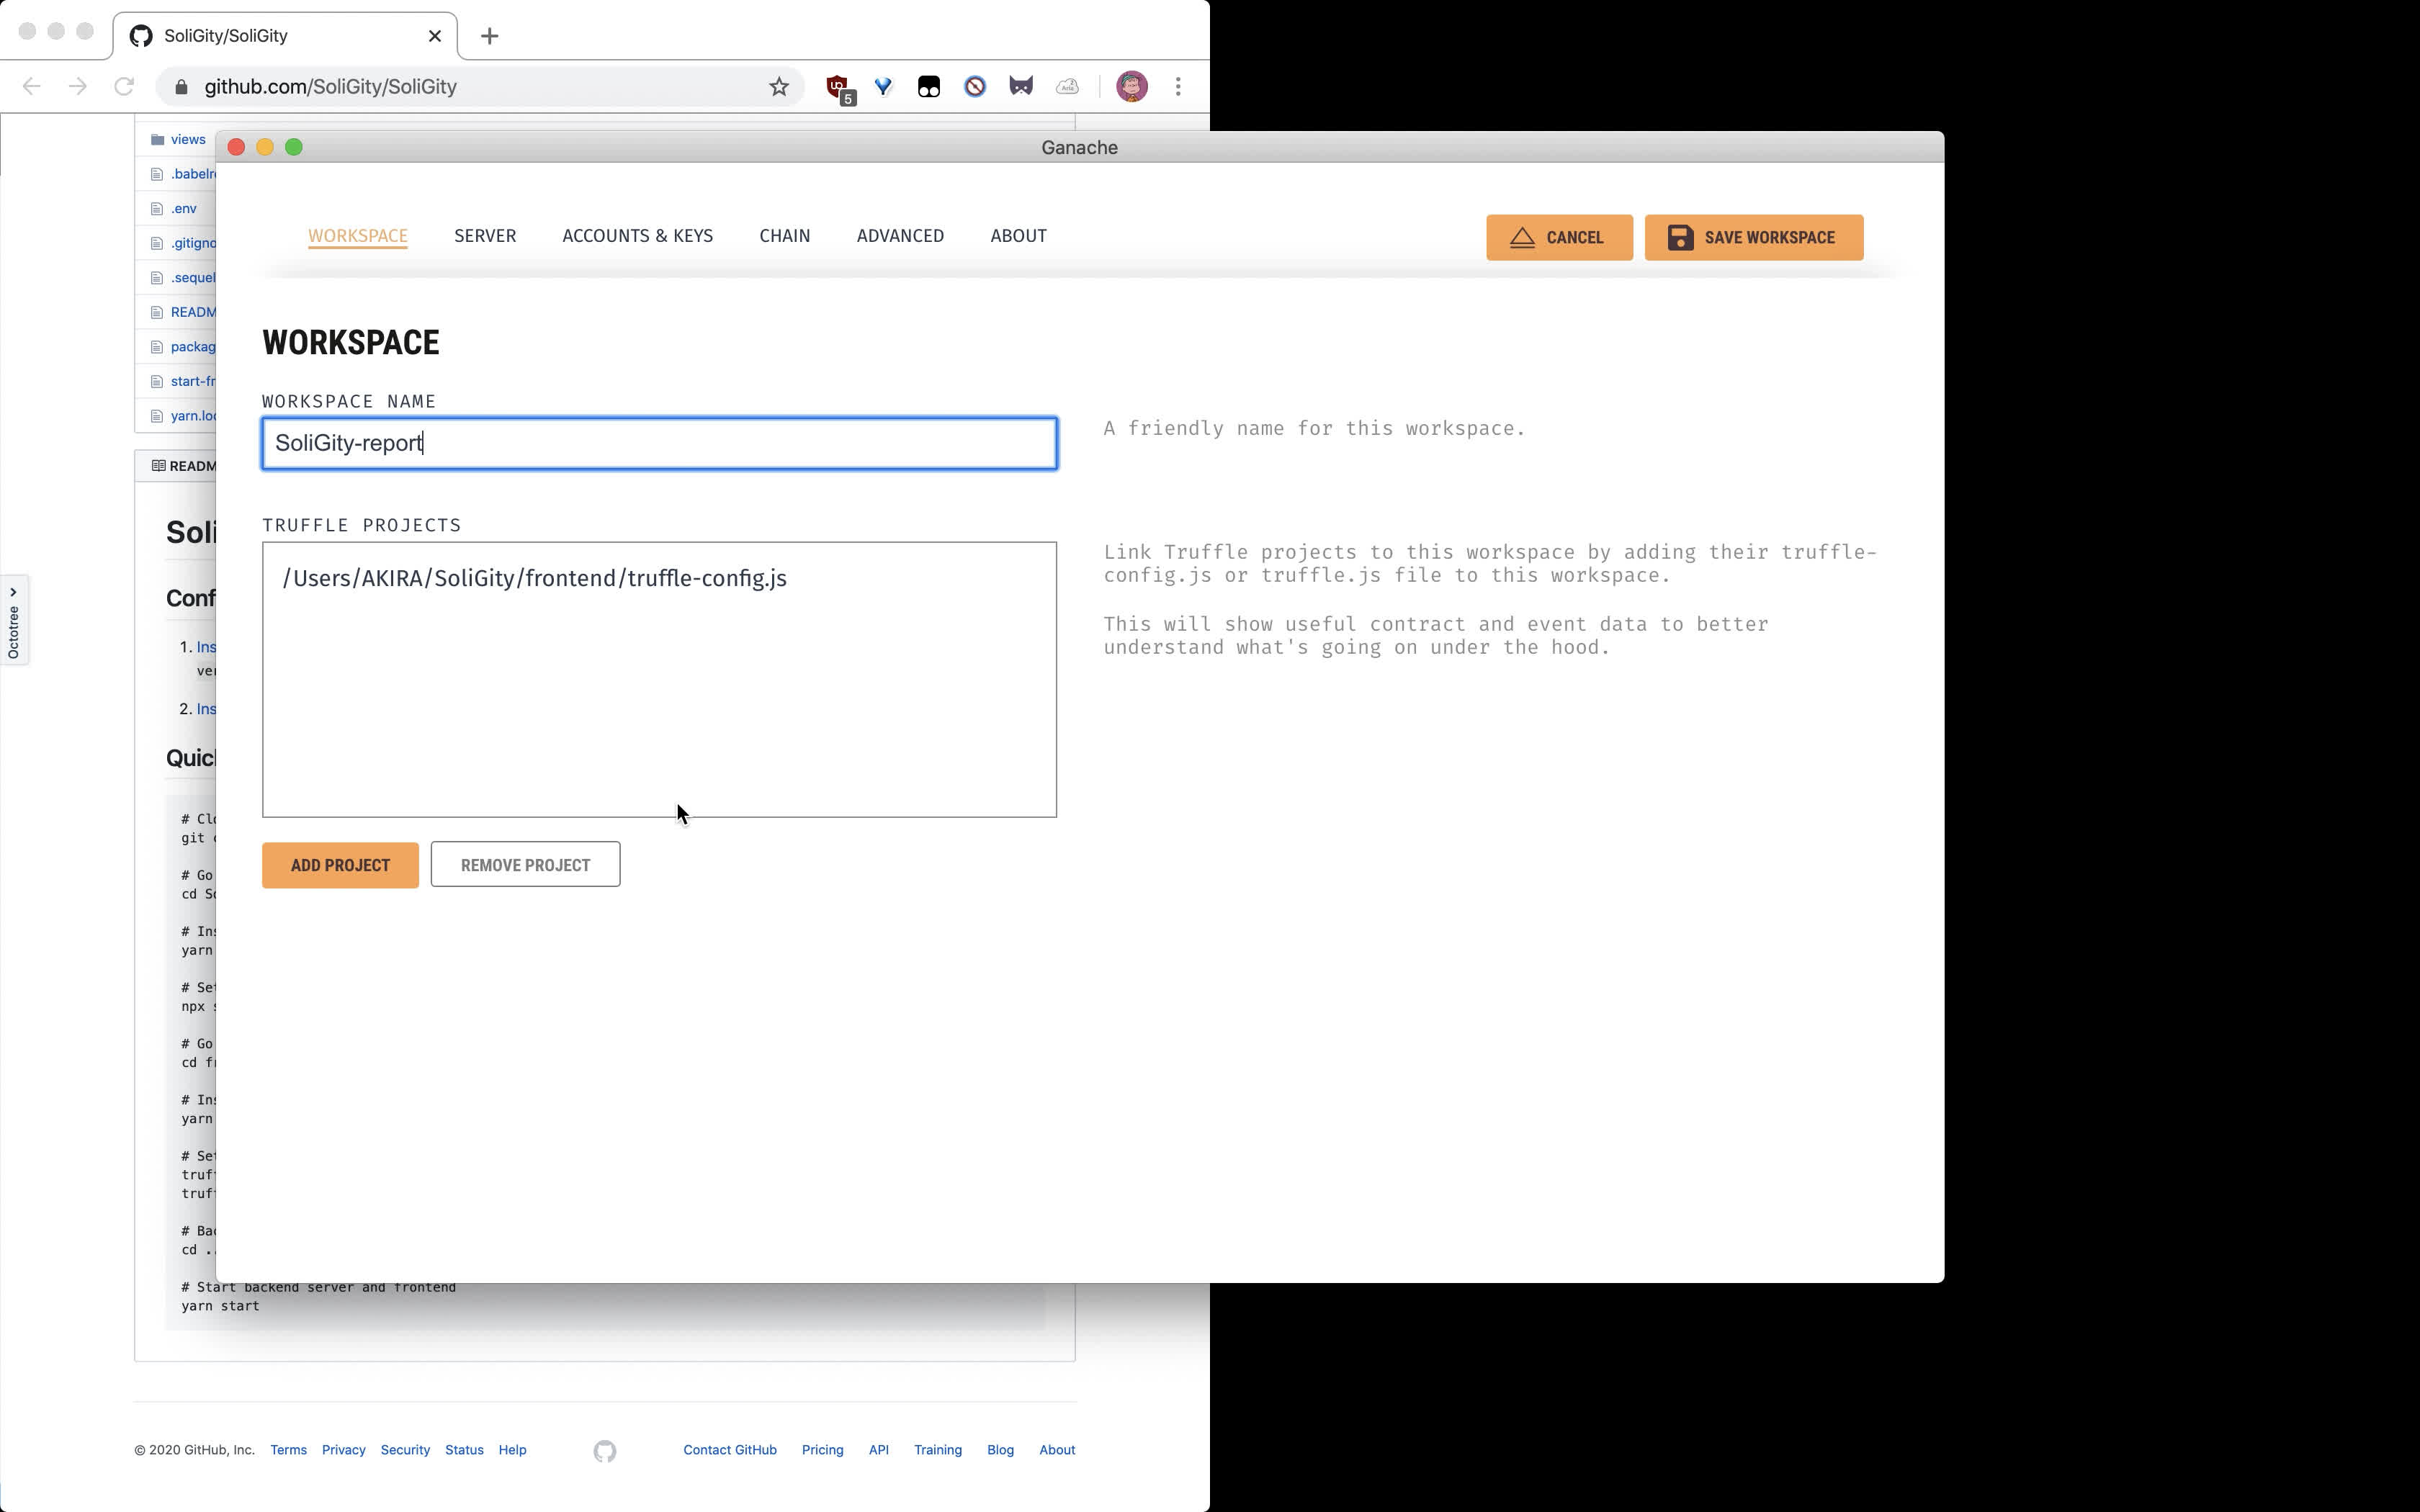
\includegraphics[width=\textwidth]{graphs/06. ganache_setup.jpg}
% 	\end{subfigure}
% 	\begin{subfigure}[t]{.45\textwidth}
% 	\captionsetup{justification   = raggedright,
%               singlelinecheck = false}
% 		\centering
% 				\caption*{\textbf{Setup Output} - \texttt{truffle migrate}}
% 		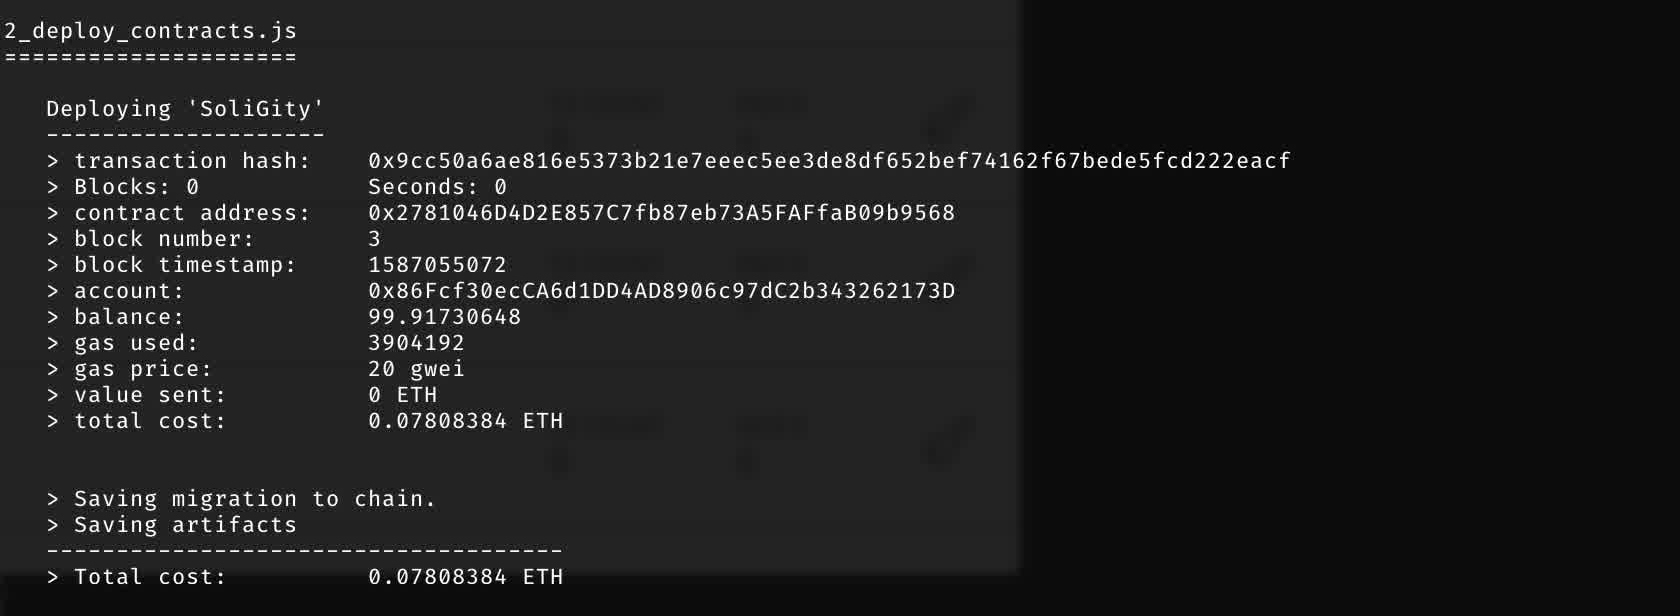
\includegraphics[width=\textwidth]{graphs/07. truffle_migrate.jpg}
% 	\end{subfigure}
% 	\begin{subfigure}[t]{.45\textwidth}
% 	\captionsetup{justification   = raggedright,
%               singlelinecheck = false}
% 		\centering
% 				\caption*{\textbf{Deployed Contract}}
% 		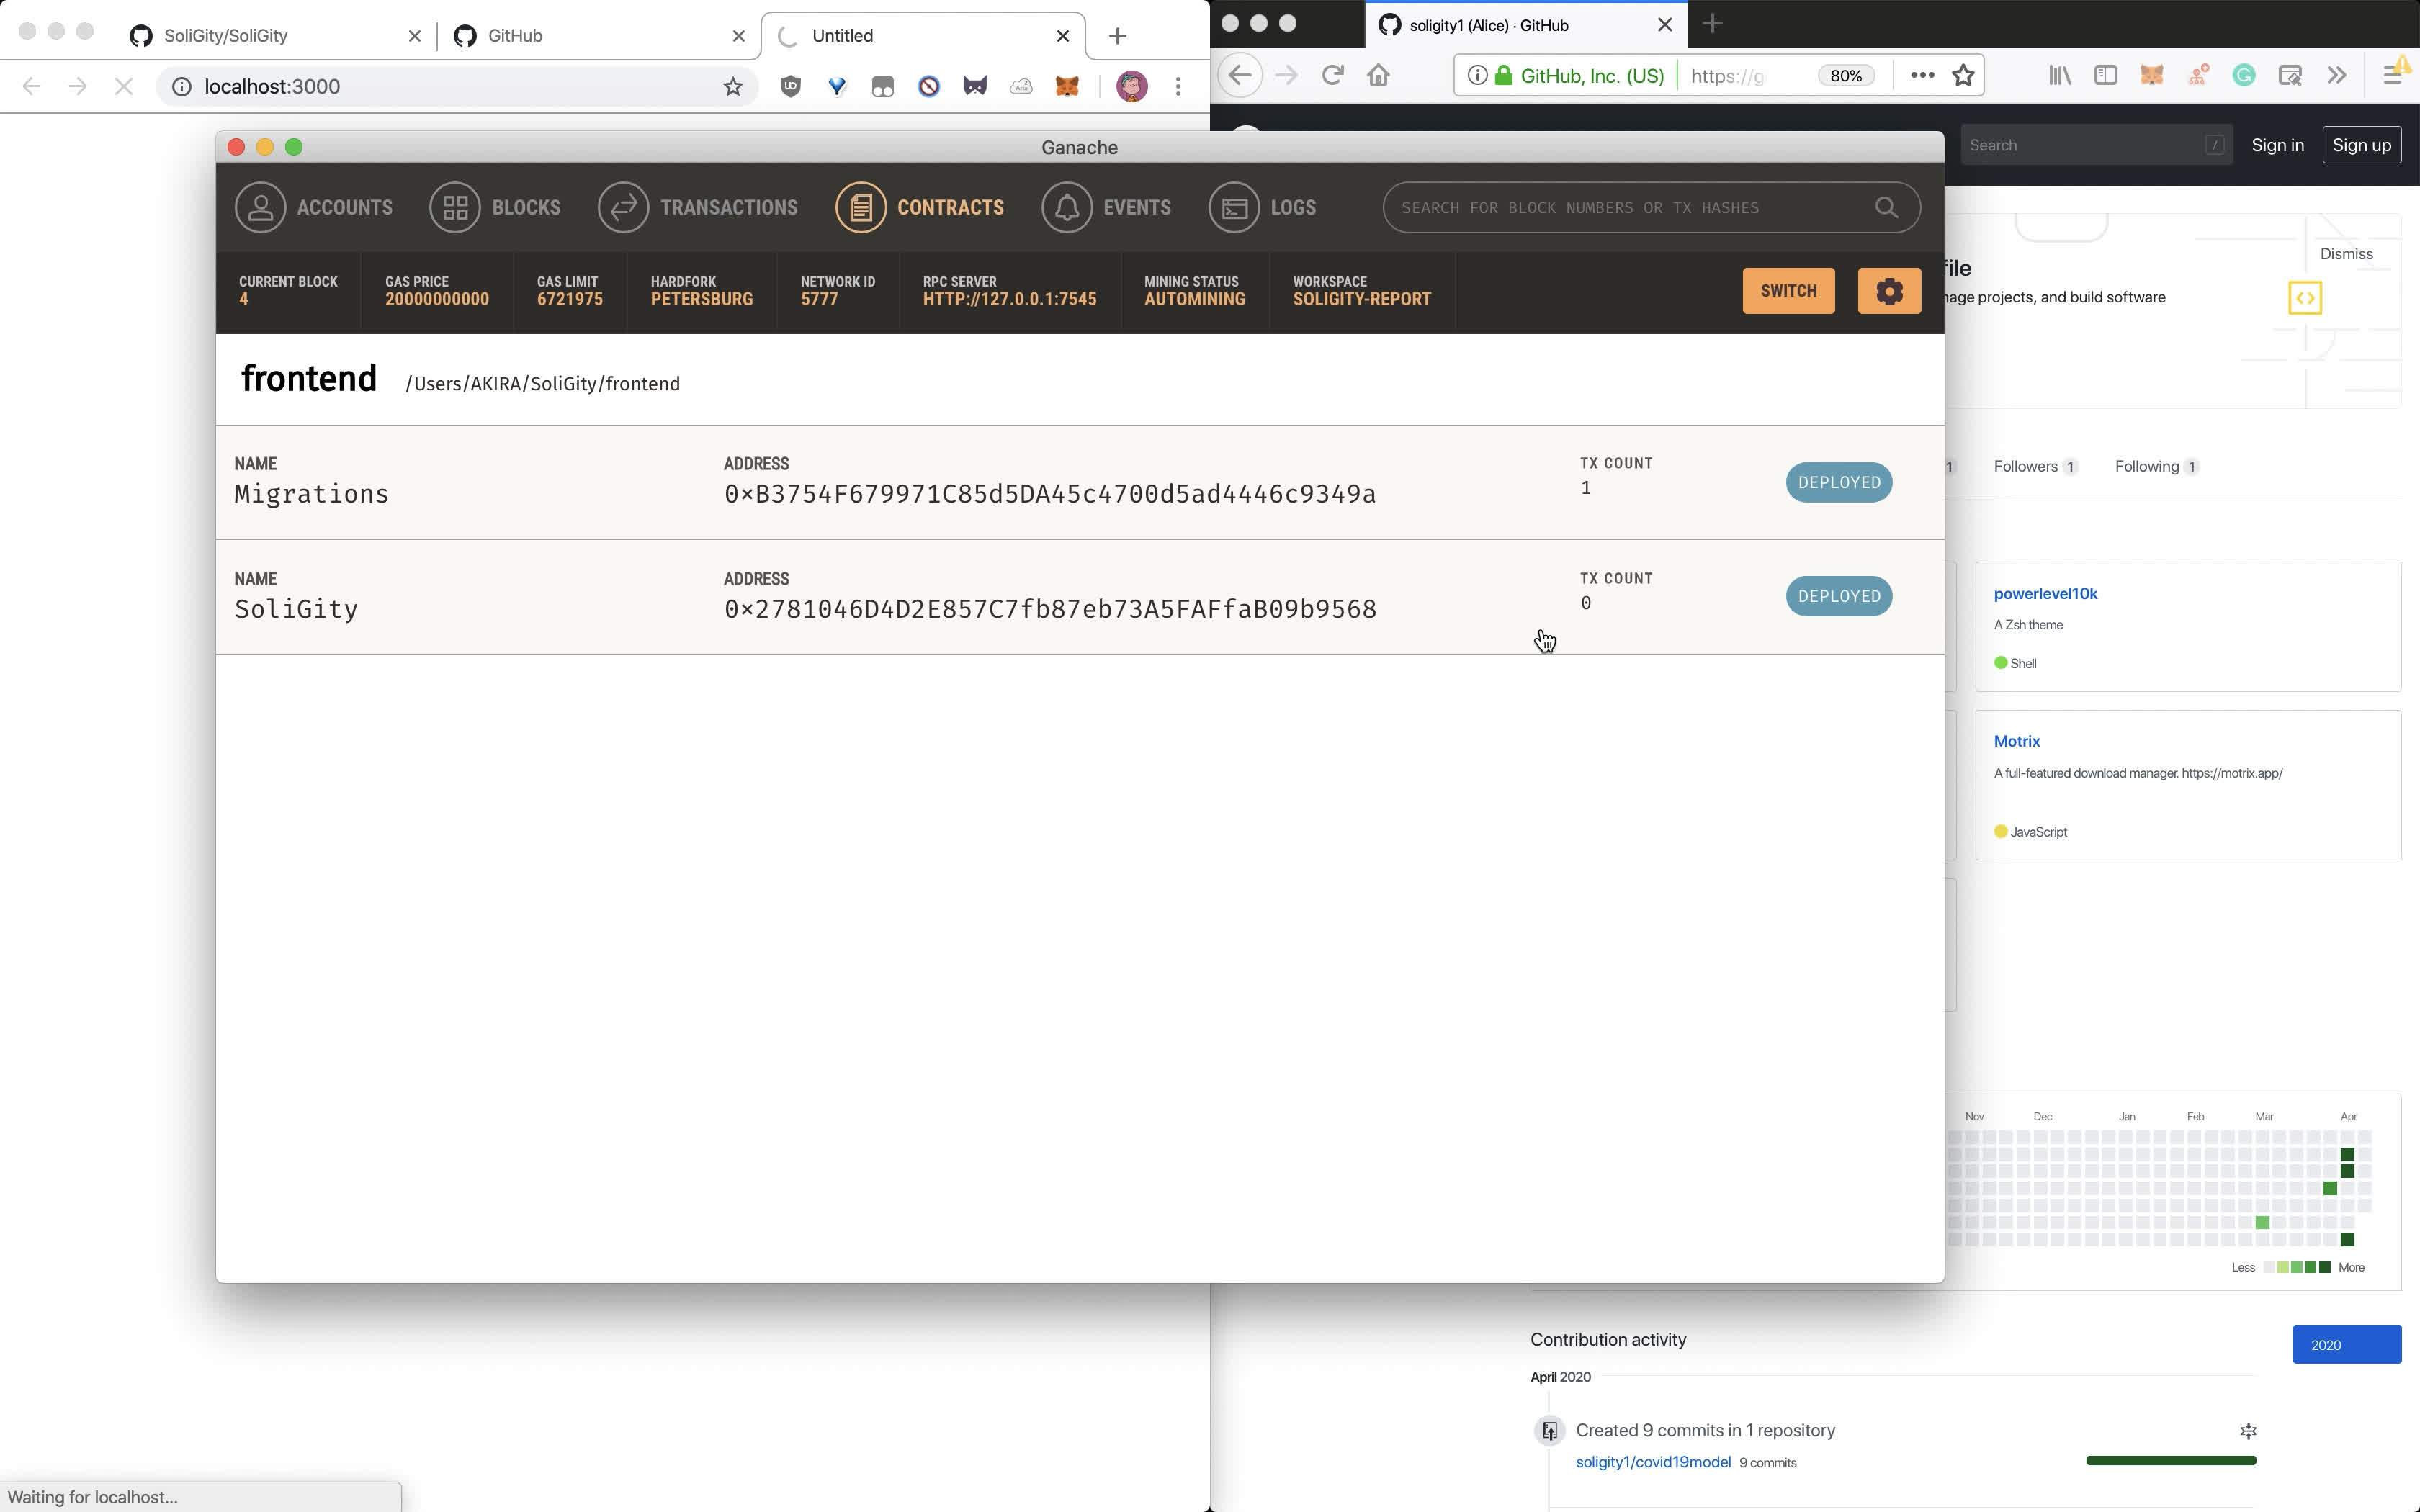
\includegraphics[width=\textwidth]{graphs/08. ganache_deployed_contract.jpg}
% 	\end{subfigure}
% 	\caption{Backend and Frontend Environment Configuration}
% \end{figure}

% \begin{figure}[H]
% 	\centering
% 	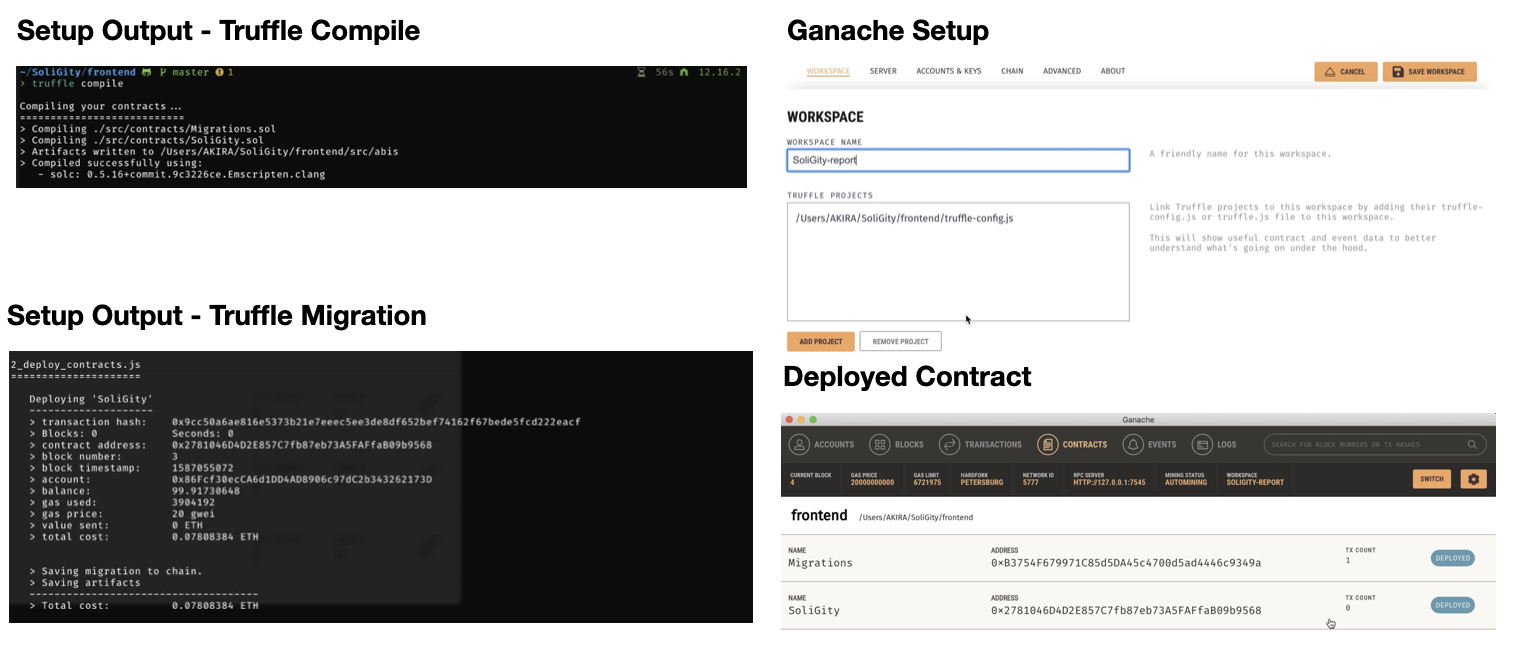
\includegraphics[width=16.5cm]{graphs/47. setup_2.png}\\
% 	\caption{Frontend - \texttt{truffle compile} and \texttt{truffle migration}}
% 	\label{fig:setup4}
% \end{figure}
The link to repository of our project is \texttt{https://github.com/soligity}. From there, you will find the step-by-step setup instructions. To test our prototype locally on a single machine, the commands in Figure~\ref{fig:setup0} are used. After cloning the repository, we need to install all the dependencies for the backend, followed by a database migration.  Then, we install the dependencies for frontend. Note that a Ganache workspace needs to be created and be kept running throughout the rest of the processes. Running \texttt{truffle compile} and \texttt{truffle migrate} will compile the smart contract and deploy it to the local Ethereum network. When all the installations and deployment are successful, we will be able to launch the web server from the SoliGity main directory by running \textit{yarn start}. The default port number used for the local host is \texttt{3000}. 

\subsubsection{Setup Accounts}
In the rest of the demo, we name the first party - Project Owner as Alice; and the second party - Contributor/Developer as Bob. To differentiate their identities easily, we use 2 separate browsers: Firefox and Chrome respectively. To accomplish the workflow, each party must have two accounts: Blockchain Account and SoliGity Website Account. 

In our local demo, the Blockchain account is obtained from the testing network served by Ganache. By selecting any two accounts (except the account indexed 0) and importing their private keys into the MetaMask - a web browser extension for accessing Ethereum enabled distributed applications, both Alice and Bob have 100 Ethereums (ETH) of balance in their wallet and are able to perform transactions within SoliGity  (Figure~\ref{fig:setup5}. Throughout the process, Ganache should remain running in the background.

\begin{figure}[H]
	\centering
	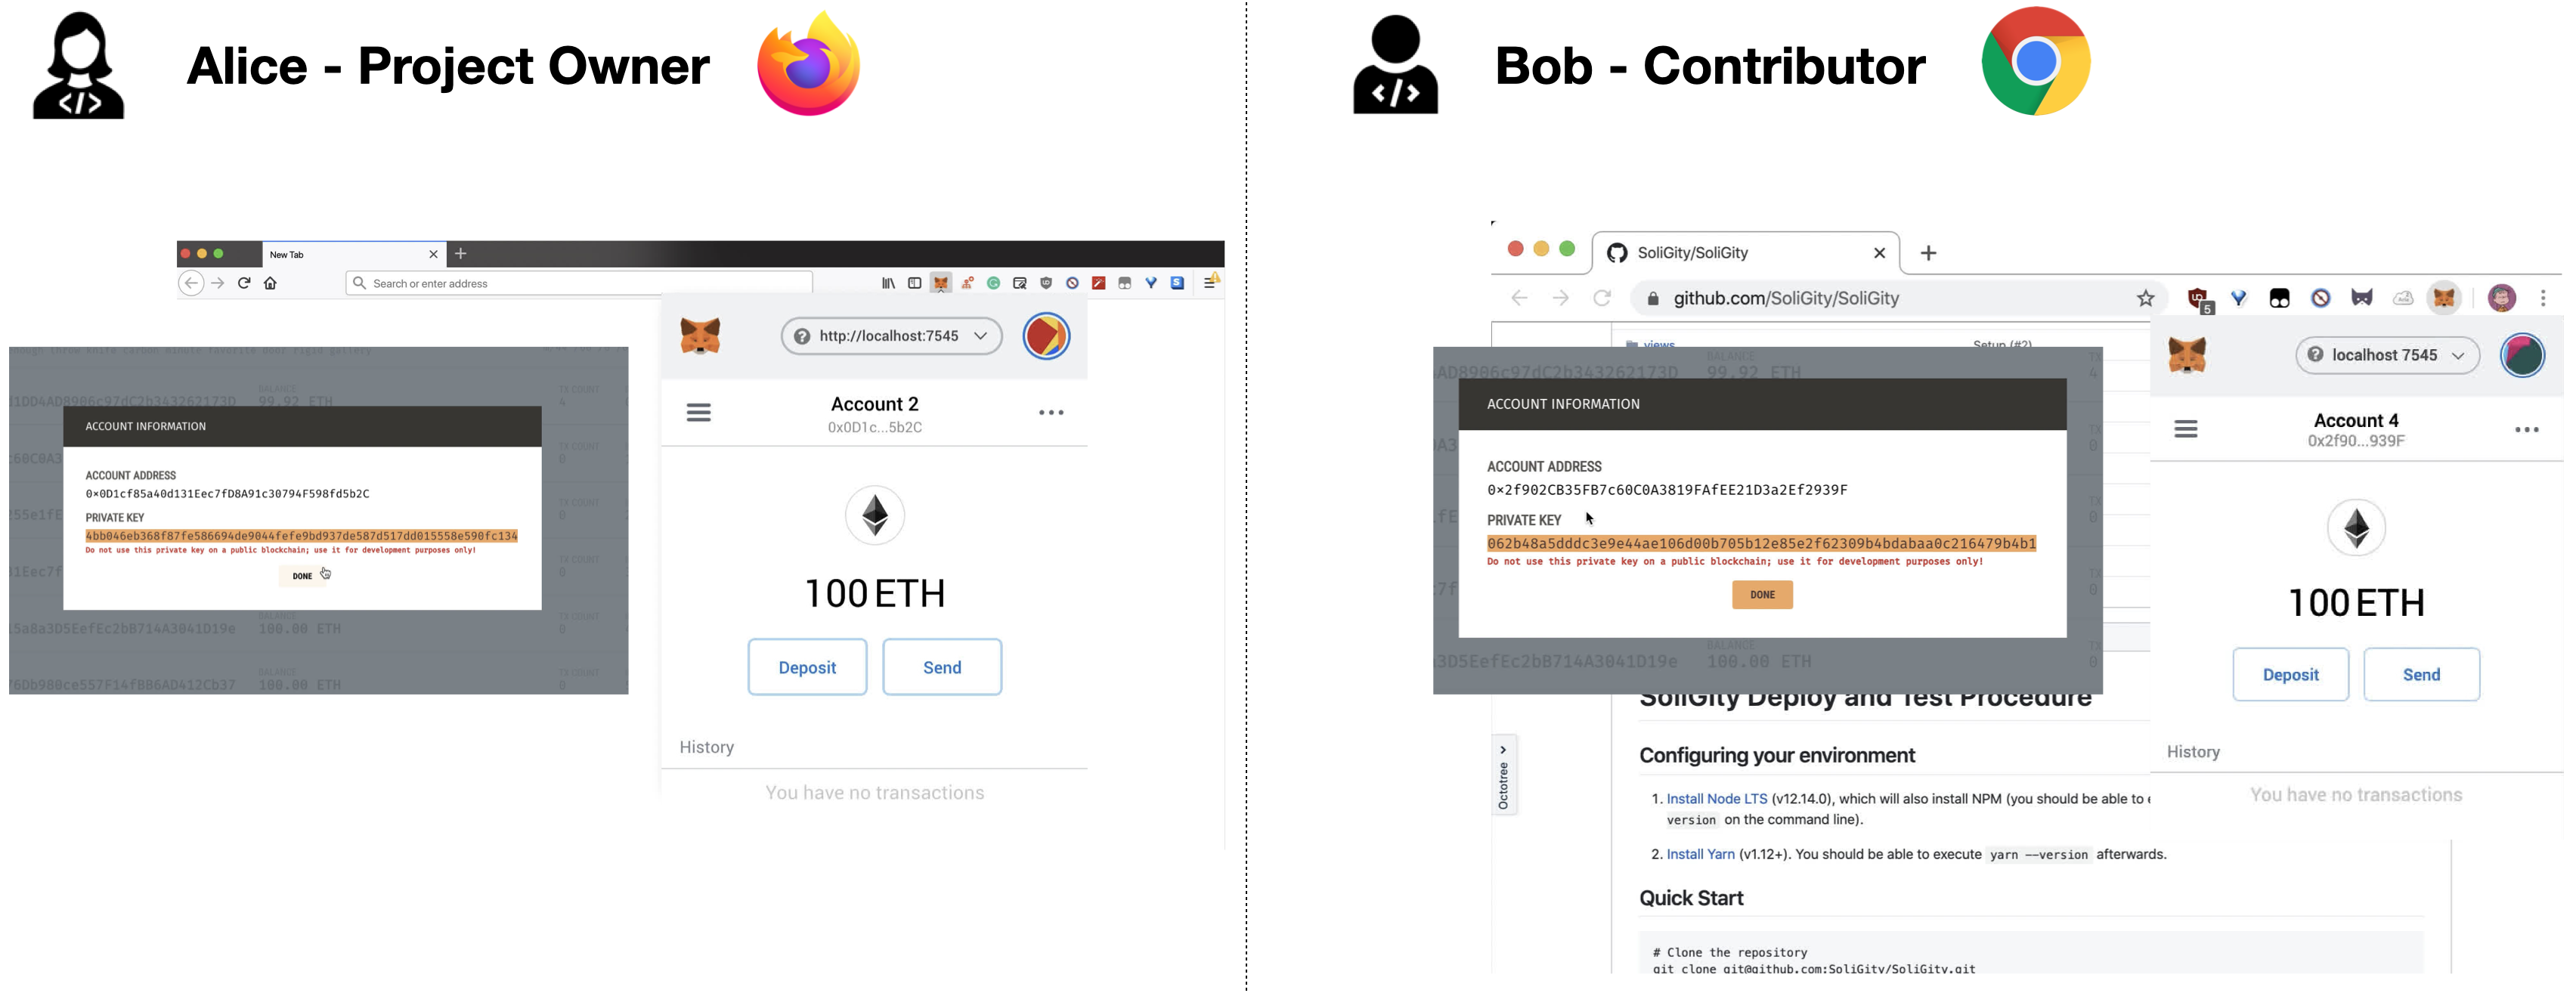
\includegraphics[width=16.5cm]{graphs/48. setup_3.png}\\
	\caption{Importing accounts into Meta Mask}
	\label{fig:setup5}
\end{figure}

The second account is required to access to the SoliGity website. After signing up an account and logging in, both Alice and Bob need to associate their GitHub accounts with their SoliGity accounts (Figure~\ref{fig:setup6}). This allows them to view all their GitHub projects (repositories) and choose whatever projects they would like everyone on SoliGity to make contributions to. The Github Integration is achieved using GitHub APIs. 

\begin{figure}[H]
	\centering
	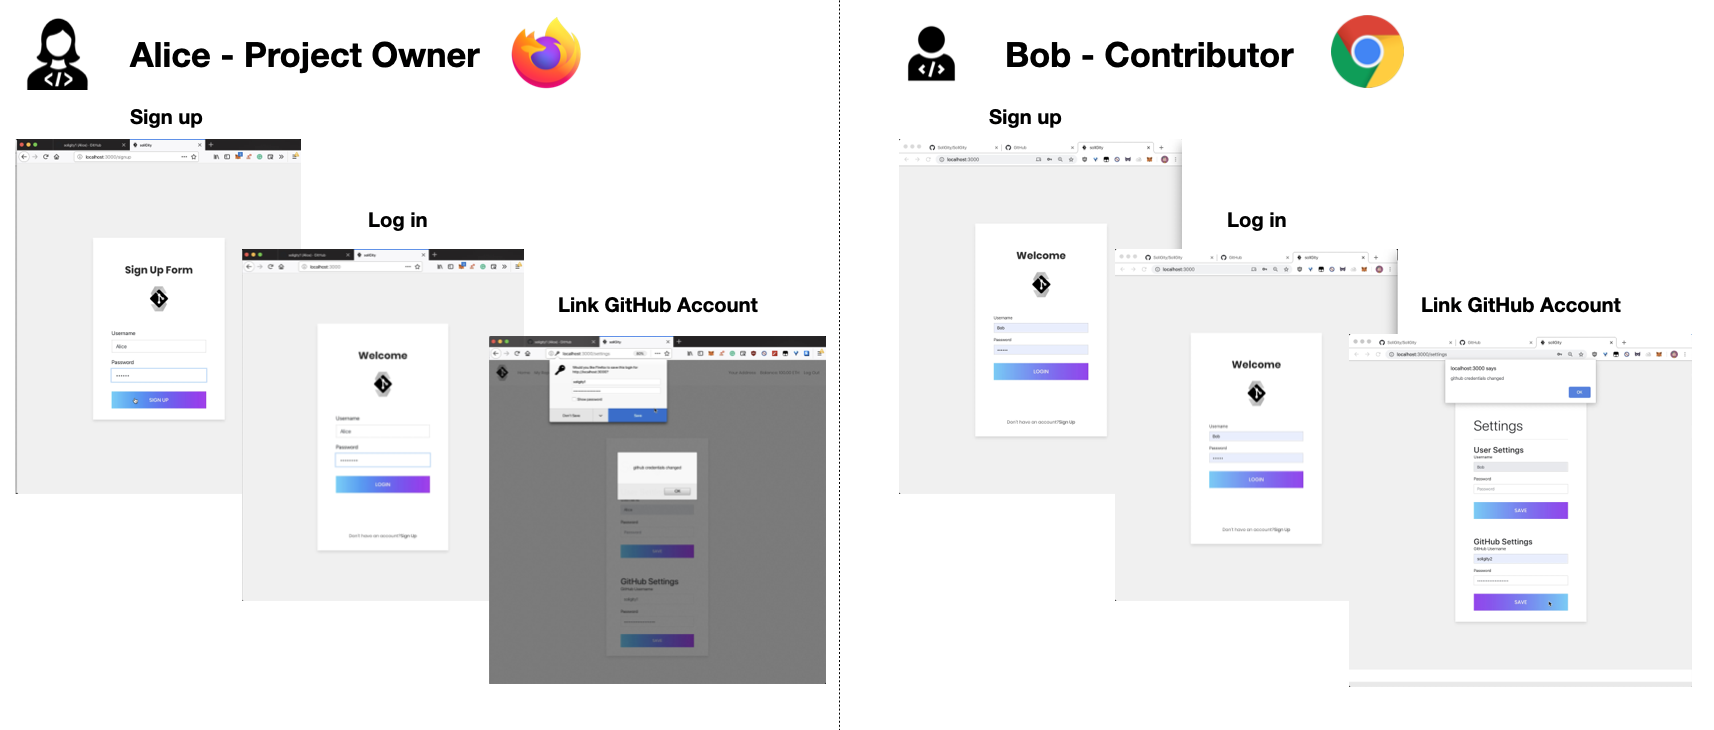
\includegraphics[width=16.5cm]{graphs/49. setup_4.png}\\
	\caption{SoliGity Account Setup}
	\label{fig:setup6}
\end{figure}

\subsection{Post Project}
\subsubsection{Post Project to Catalog}
Project Catalog is a page where any registered SoliGity user is able to discover the participating projects. Since the web application is started from fresh and no one has posted any projects to SoliGity, the Project Catalog is empty (Figure~\ref{fig:post1} Left). As a project owner, Alice would like someone else on SoliGity to help her add new features and fixing some bugs to 2 projects she owns. Therefore, she chooses two projects \texttt{covid19model} and \texttt{DeepPiCar} from her Repository list and presses the \textit{Post to Catalog Button}. Note that we also use the DApp to manage the posted project on Project Catalog, meaning that posting a project to SoliGity will be recorded on the blockchain using the smart contract. That's why Alice need to pay a small amount of Gas fee for computation (Figure~\ref{fig:post1} Middle). After the projects are posted, they are visible on the Project Catalog page (Figure~\ref{fig:post1} Right). Note that these posted projects are also visible to Bob.
\begin{figure}[H]
	\centering
	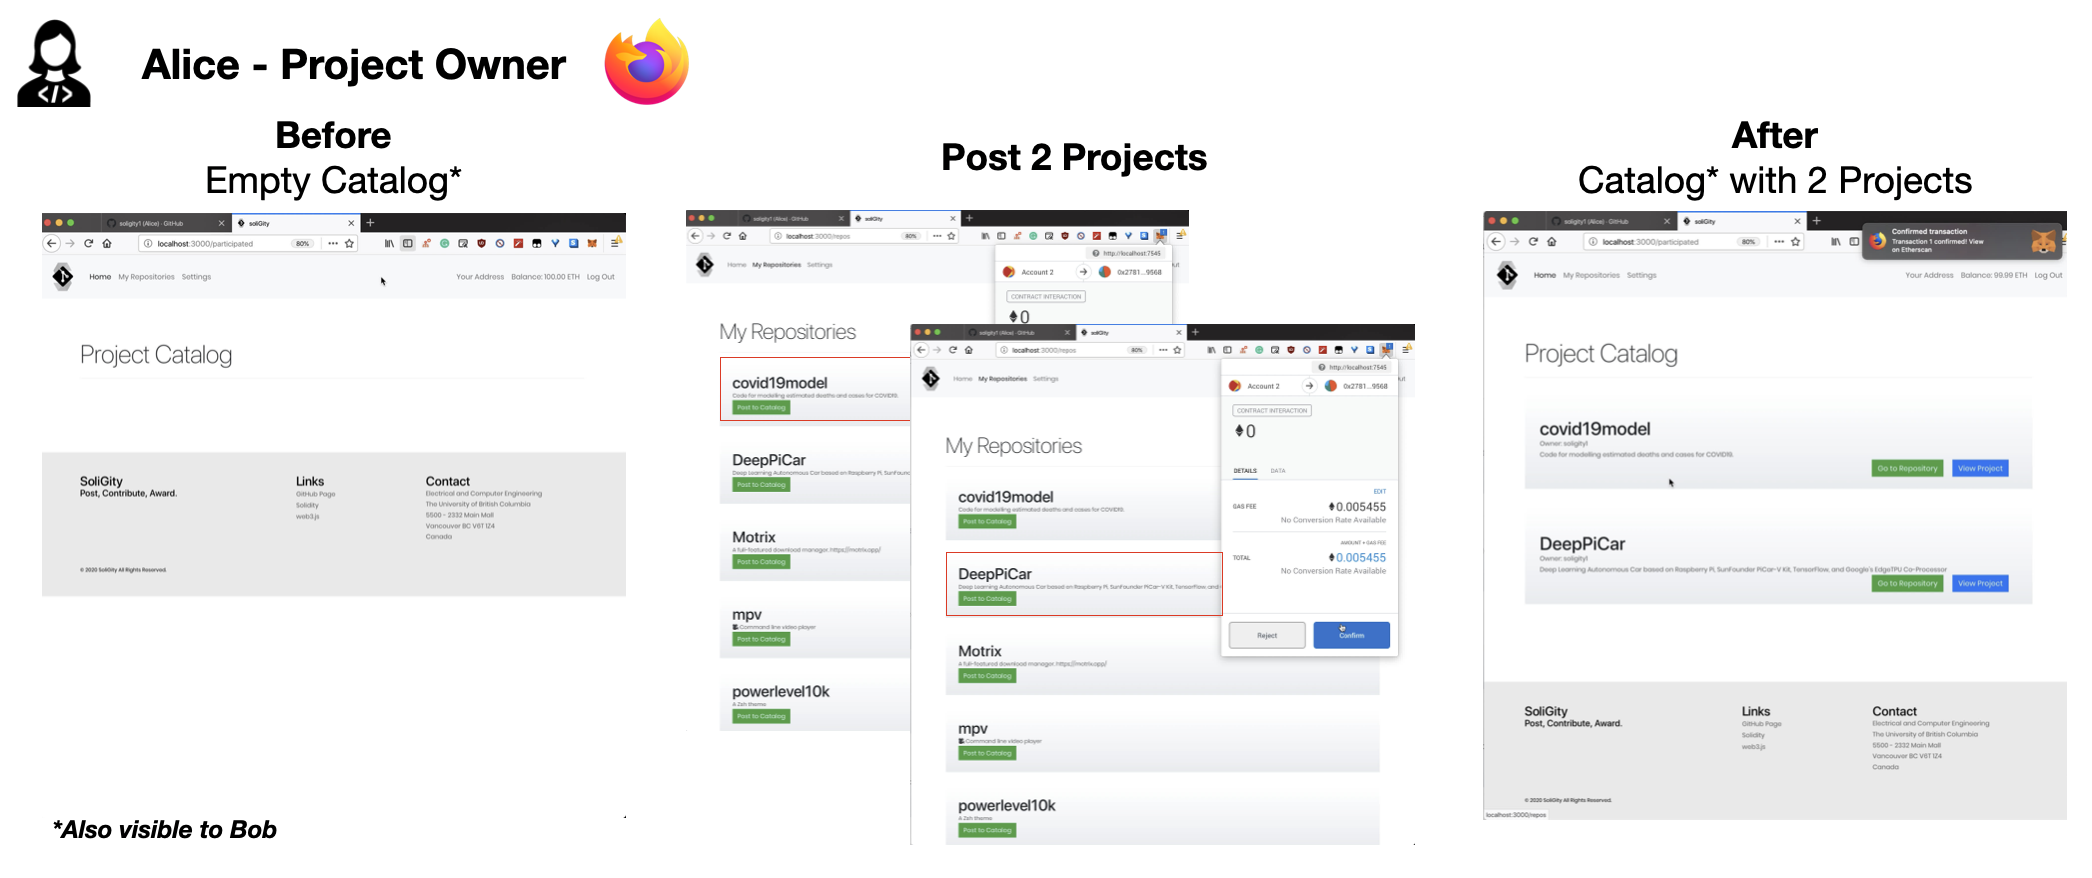
\includegraphics[width=16.5cm]{graphs/50. post_1.png}\\
	\caption{Project owner posting 2 projects to Project Catalog}
	\label{fig:post1}
\end{figure}

\subsubsection{Create Issues}
In order to let others know precisely what changes need to be made for her project and how much she is willing to pay for the contribution, Alice needs to create issues in the Project Description page, which can be accessed by clicking the \texttt{View Project} button from the Project Catalog page (Figure~\ref{fig:post2} Left). As described in Section~\ref{section:usecaseworkflow}, issues created in SoliGity are associated with a status, in this case \texttt{Accepting Contribution}. (Figure~\ref{fig:post2} Middle). The issues created within SoliGity will also be propagated to GitHub (Figure~\ref{fig:post2} Right). Issues created outside SoliGity are not applicable to the rewarding mechanism.
\begin{figure}[H]
	\centering
	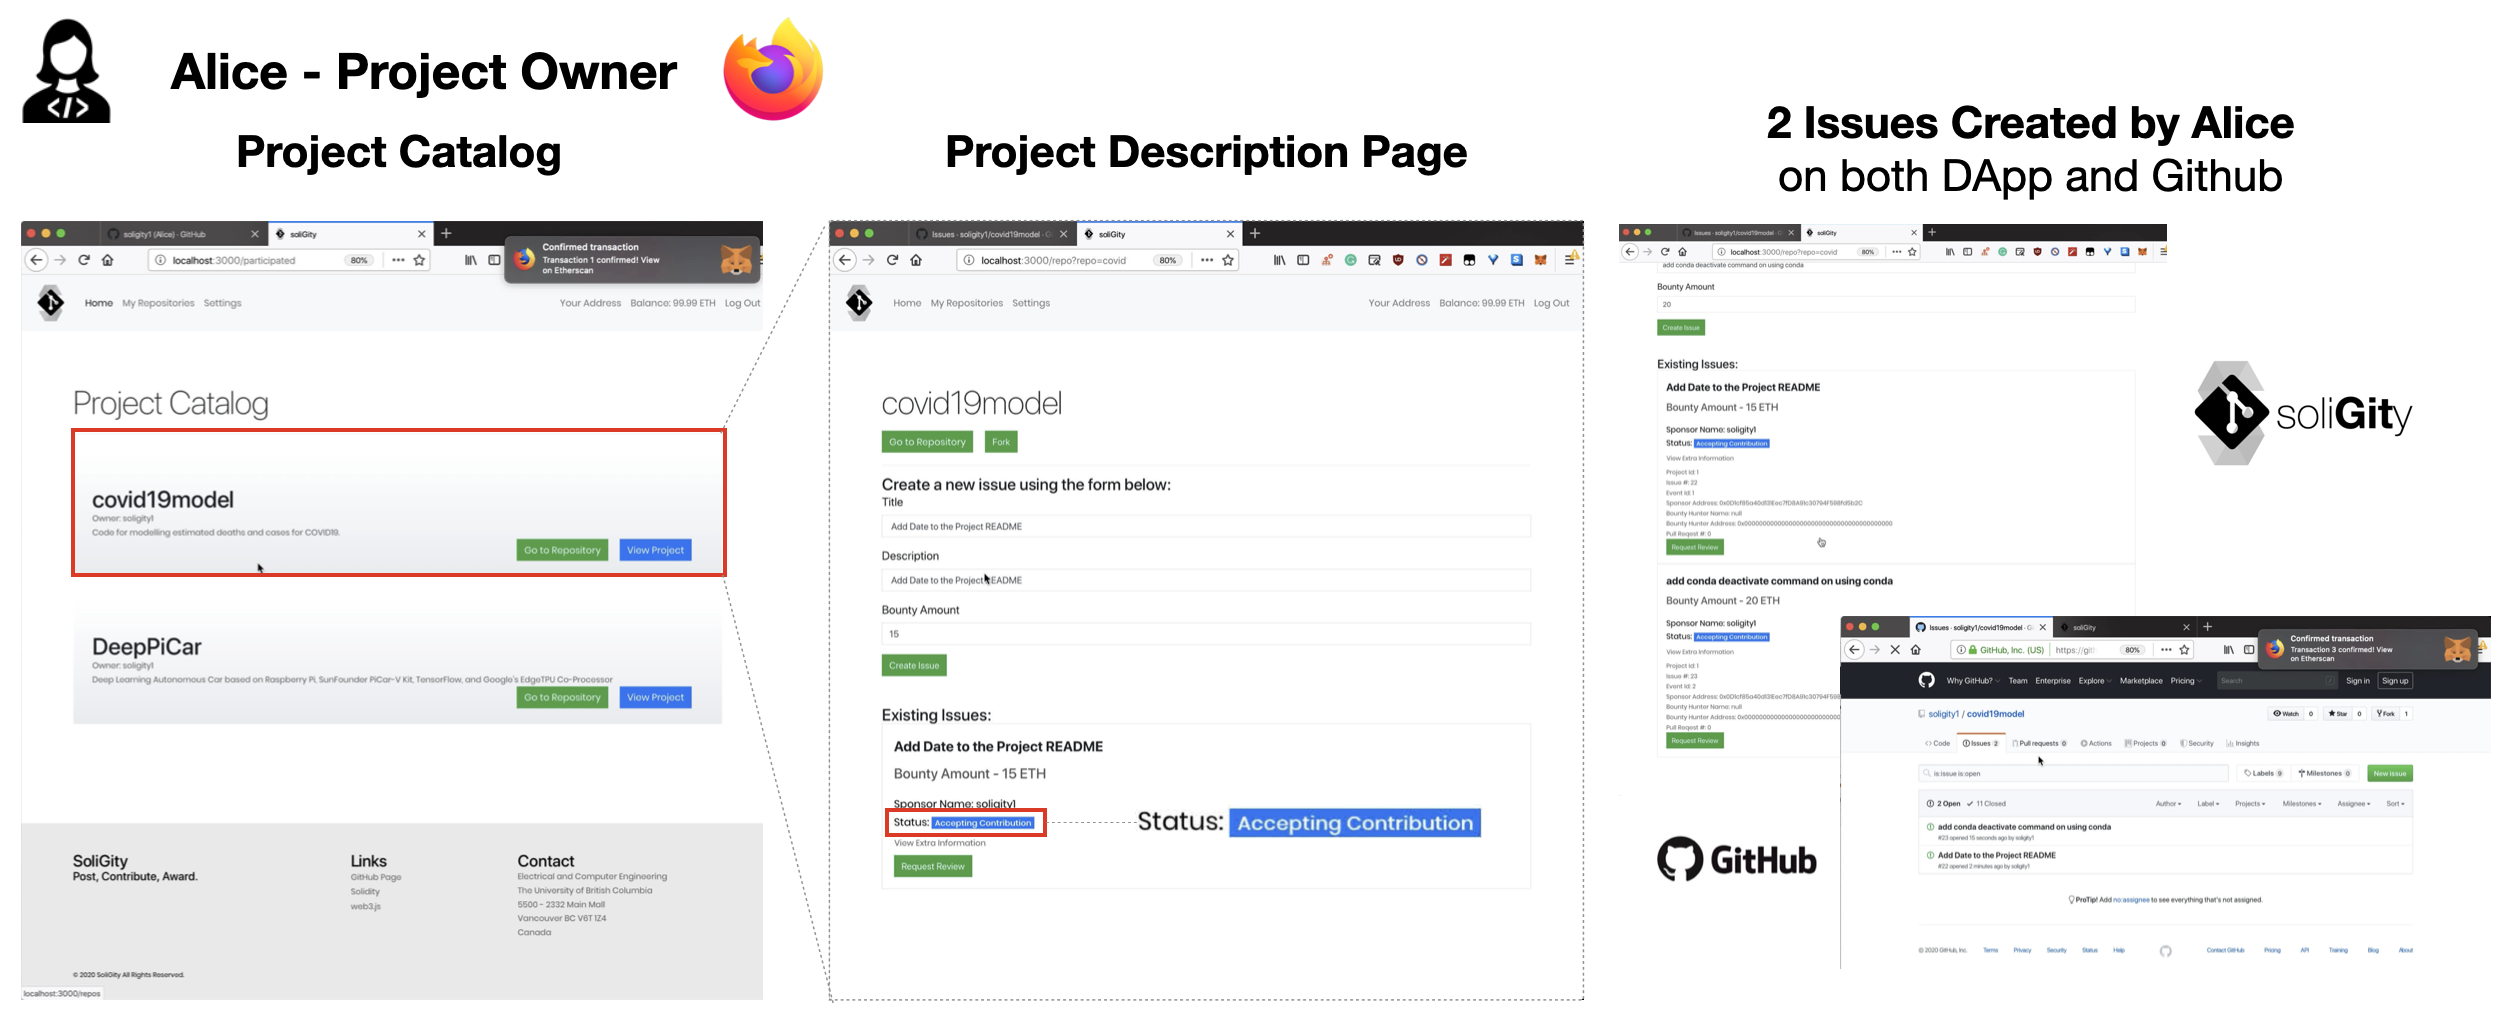
\includegraphics[width=16.5cm]{graphs/51. post_2.png}\\
	\caption{Project owner creating 2 issues for a project}
	\label{fig:post2}
\end{figure}

\subsection{Discover Project}
As a contributor, Bob browses through all the available projects posted on the Project Catalog and chooses the projects he would like to be part of. In this case, he decides to work on the \texttt{covid19model}, so the website takes him to the project description page, where he could find the issues with status \texttt{Accepting Contribution} created by Alice earlier (Figure~\ref{fig:discover1} Left and Middle). Once Bob decides to make contributions, he can fork the project into his own GitHub account by pressing the \textit{Fork} button (Figure~\ref{fig:discover1} Middle and Right). The \textit{Fork} button is a shortcut that invokes the GitHub API.

\begin{figure}[H]
	\centering
	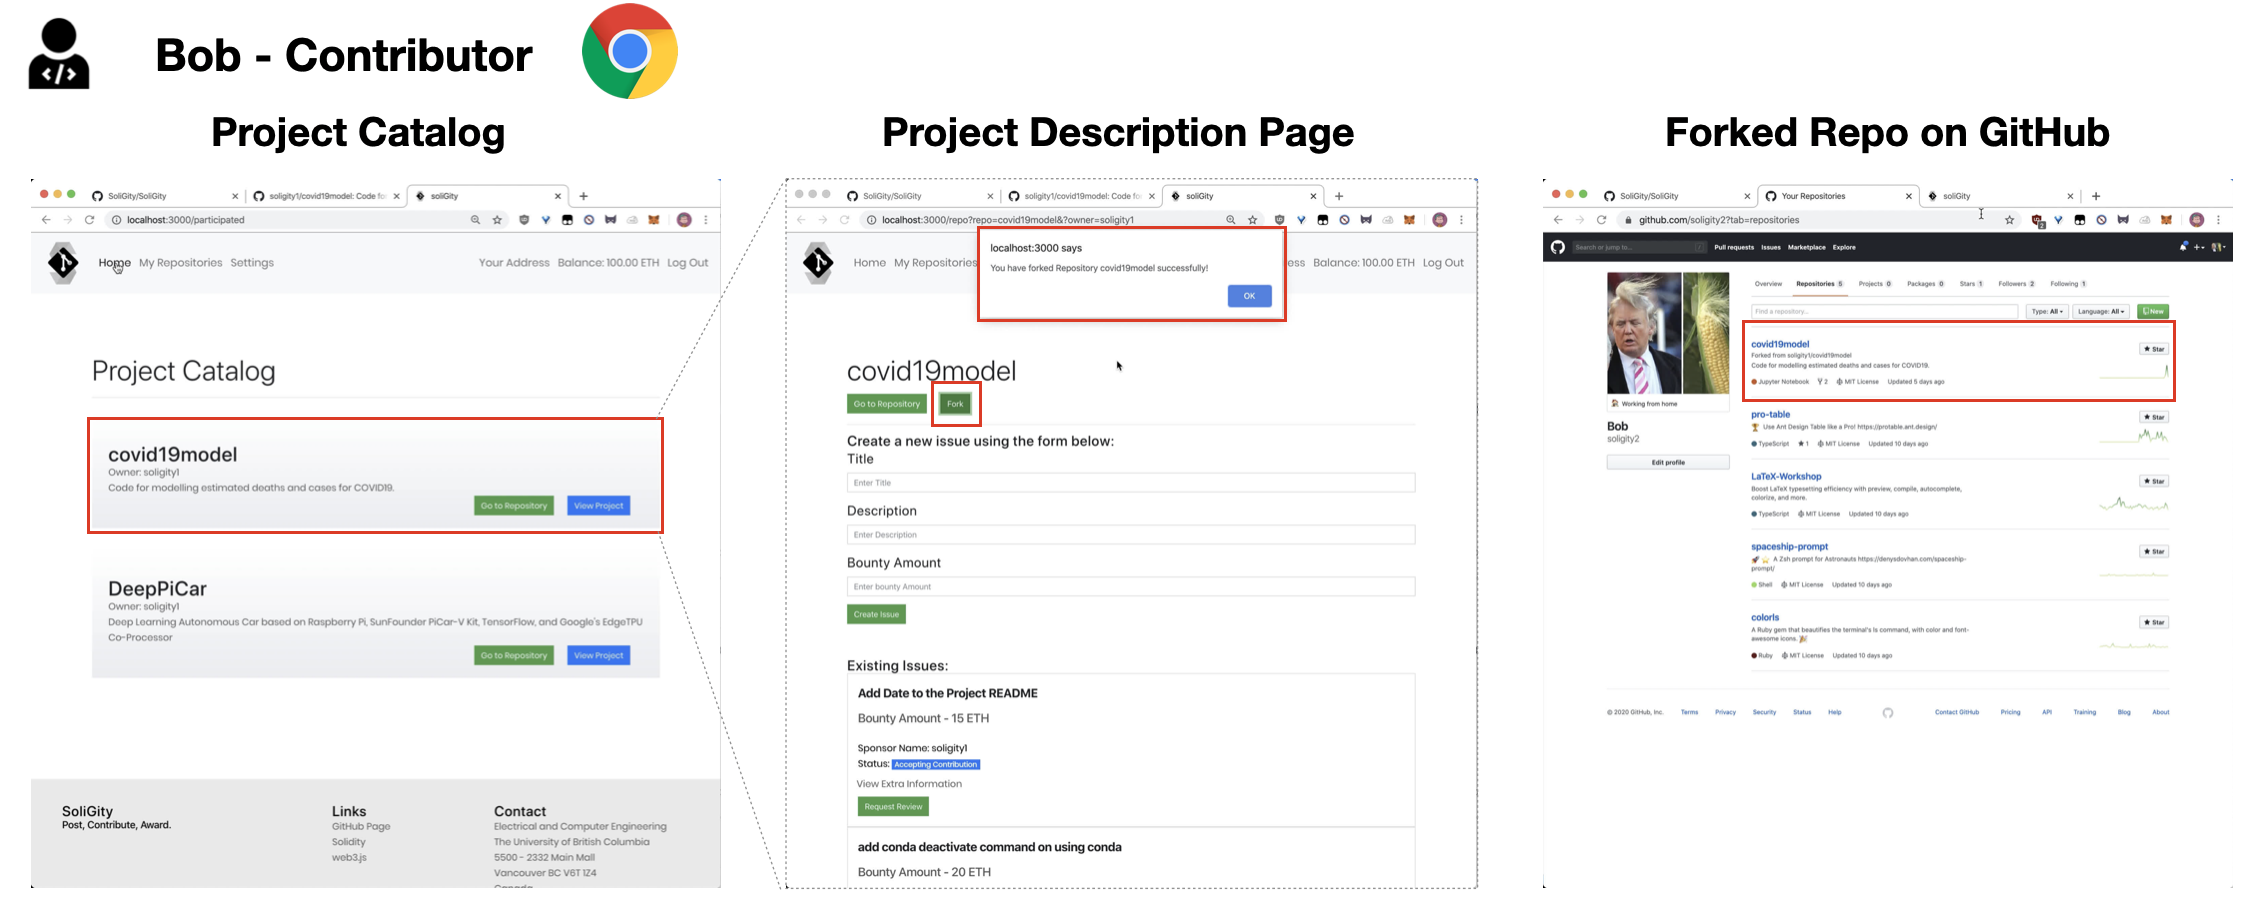
\includegraphics[width=16.5cm]{graphs/52. discover_1.png}\\
	\caption{Contributor discovering projects and choosing an issue to work on}
	\label{fig:discover1}
\end{figure}

\subsection{Making Contribution}
Bob makes changes to the project in the Forked repository so it will not affect anything on Alice's original repo. In this demo, Bob is working on an issue entitled \textit{Add Date to the Project README}. Figure~\ref{fig:contribute1} Left shows the change that Bob has made. Once Bob finishes his work, he presses the \textit{Request Review} button from the Project Description page. Doing so triggers two events: i) the issue status on SoliGity is changed from \textit{Accepting Contribution} to \textit{Pending Approval}; ii) a Pull Request is made on GitHub for Alice to review the changes (Figure~\ref{fig:contribute1} Middle and Right).  This simple demonstrates how easy and intuitive the process is. While this demo shows that the changes are made right from GitHub website, in real-world scenarios, users will follow the original Git workflow they are familiar with, such as using GUI applications or command prompts.

\begin{figure}[H]
	\centering
	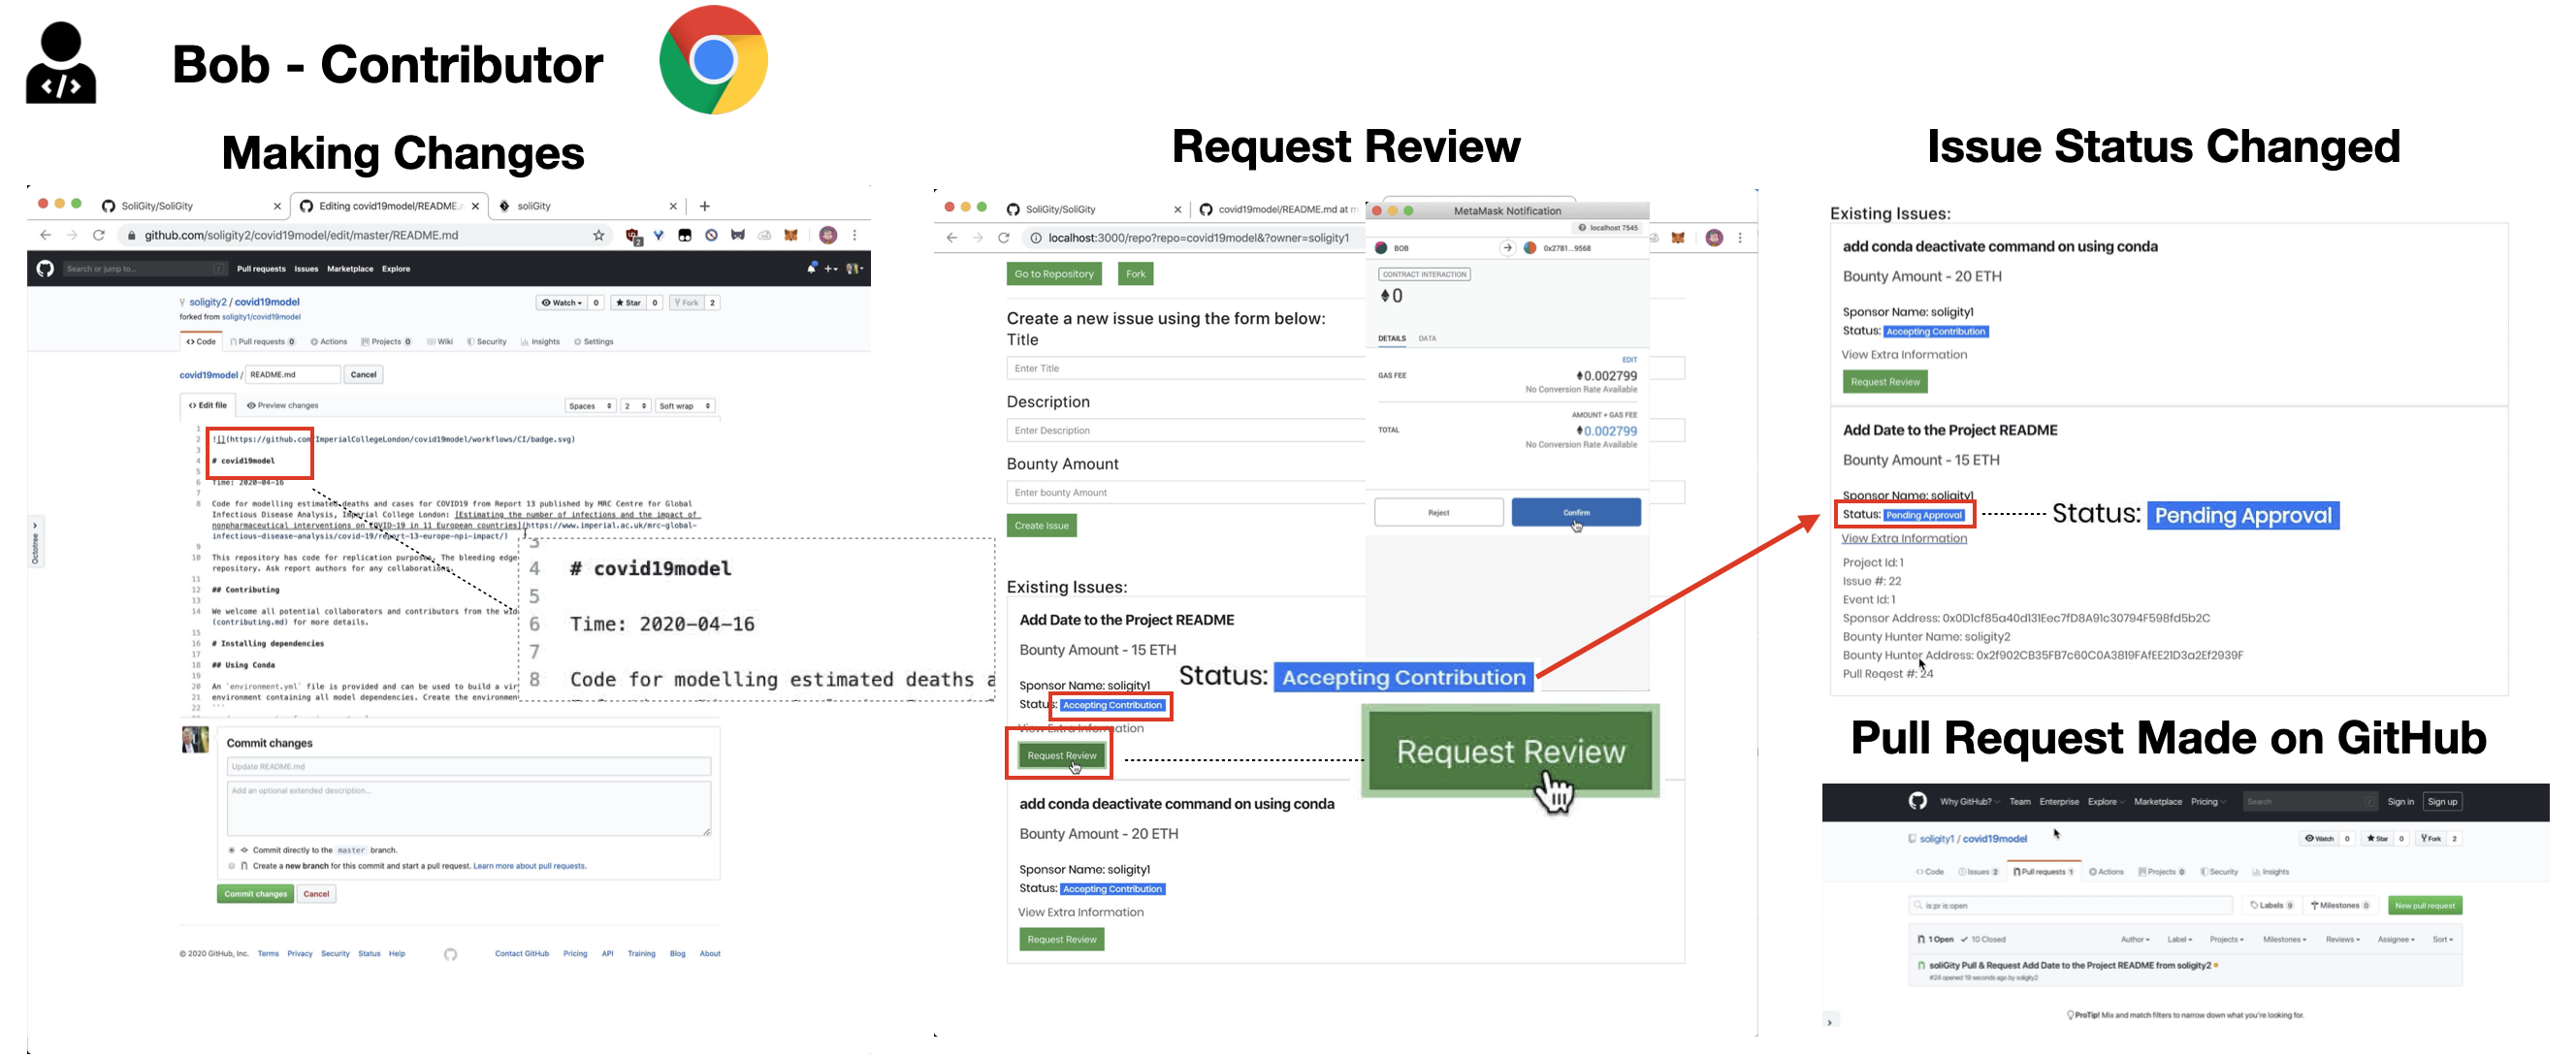
\includegraphics[width=16.5cm]{graphs/53. contribute_1.png}\\
	\caption{Contributor making changes and request for review}
	\label{fig:contribute1}
\end{figure}

\subsection{Rewarding Contribution}
\subsubsection{Reject Pull Request}
If Alice is not satisfied with Bob's work and decided to look for someone else to work on it, she can reject the Pull Request. Doing so will turn the issue back to \textit{Accepting Contribution} state, and the Bounty amount 15 ETH will not be transferred to Bob. As the state transition is written to Blockchain, Alice needs to pay for the Gas fee (Figure~\ref{fig:reward1}). 

\begin{figure}[H]
	\centering
	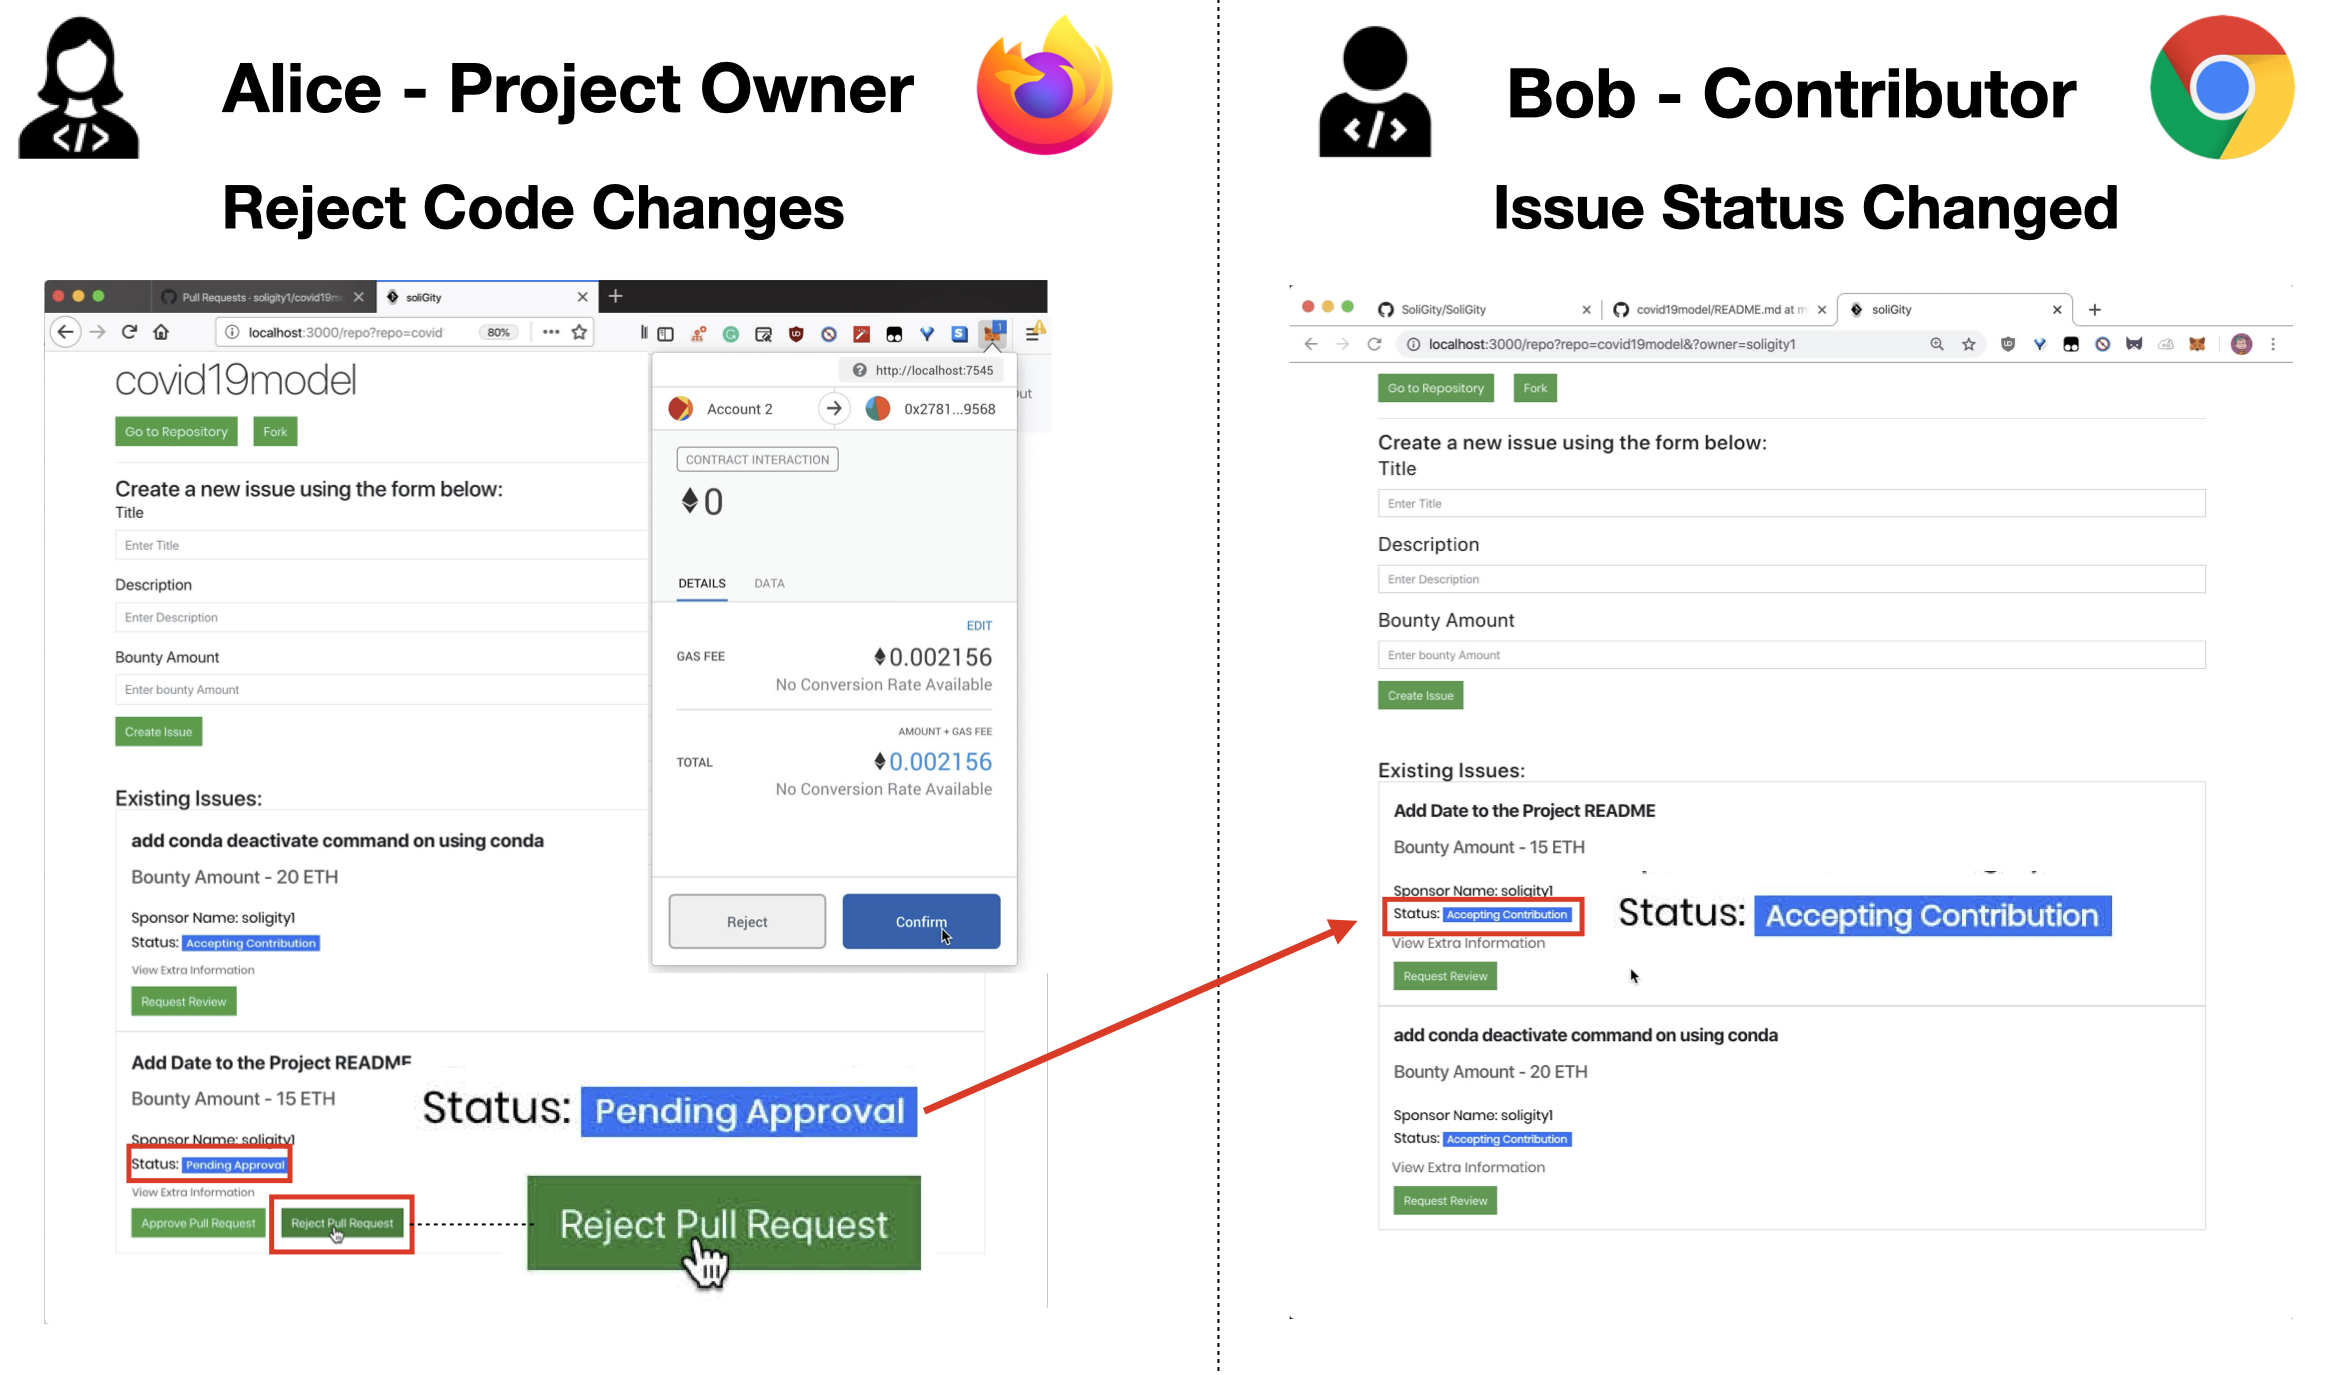
\includegraphics[height=7cm]{graphs/54. reward_1.png}\\
	\caption{Project owner rejecting code change}
	\label{fig:reward1}
\end{figure}

\subsubsection{Approve Pull Request}
If Alice is satisfied with Bob's work, she can press the \textit{Approve Pull Request} button. As discussed in Section ~\ref{section:usecaseworkflow}, doing so triggers three events: i) Bob's work is merged to Alice's original repo and the issue is closed (Figure~\ref{fig:reward2}); ii) The bounty 15 ETH is transferred from Alice's account to Bob's Account, resulting in 84.98 ETH in Alice's wallet and 114.99 ETH in Bob;'s wallet; (iii) The issue status is changed from \textit{Pending Approval} to \textit{Done}. As the state transition is written to Blockchain, there is also Gas fee in the transaction (Figure~\ref{fig:reward2}). The GitHub APIs allow the user to perform the approval actions without switching back and forth between SoliGity and GitHub, dramatically reduced confusions and the probability of human errors.    

\begin{figure}[H]
	\centering
	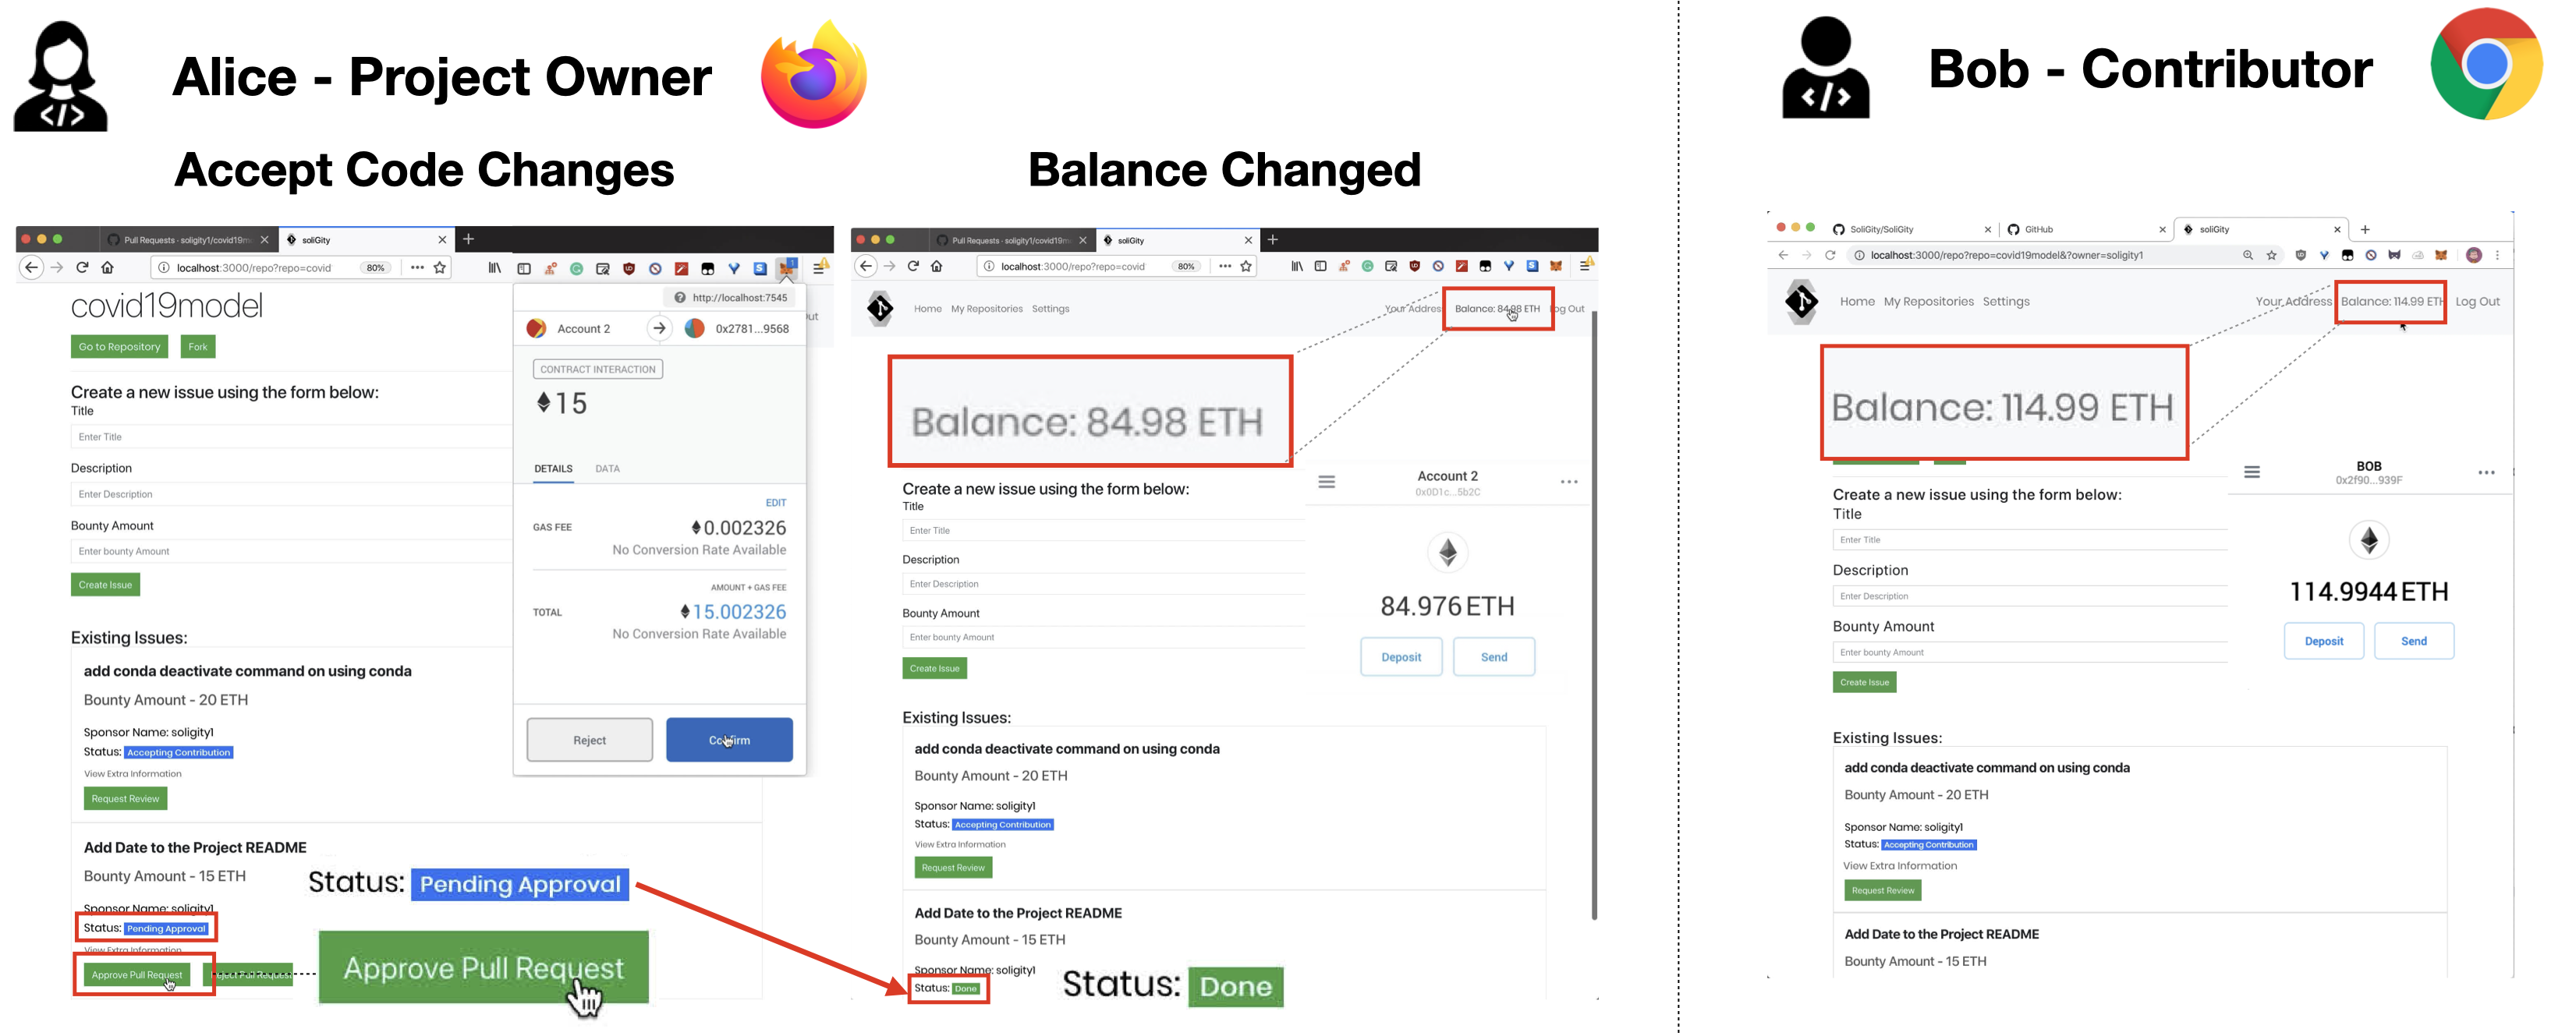
\includegraphics[width=16cm]{graphs/55. reward_2.png}\\
	\caption{Project owner approving code change}
	\label{fig:reward2}
\end{figure}

\begin{figure}[H]
	\centering
	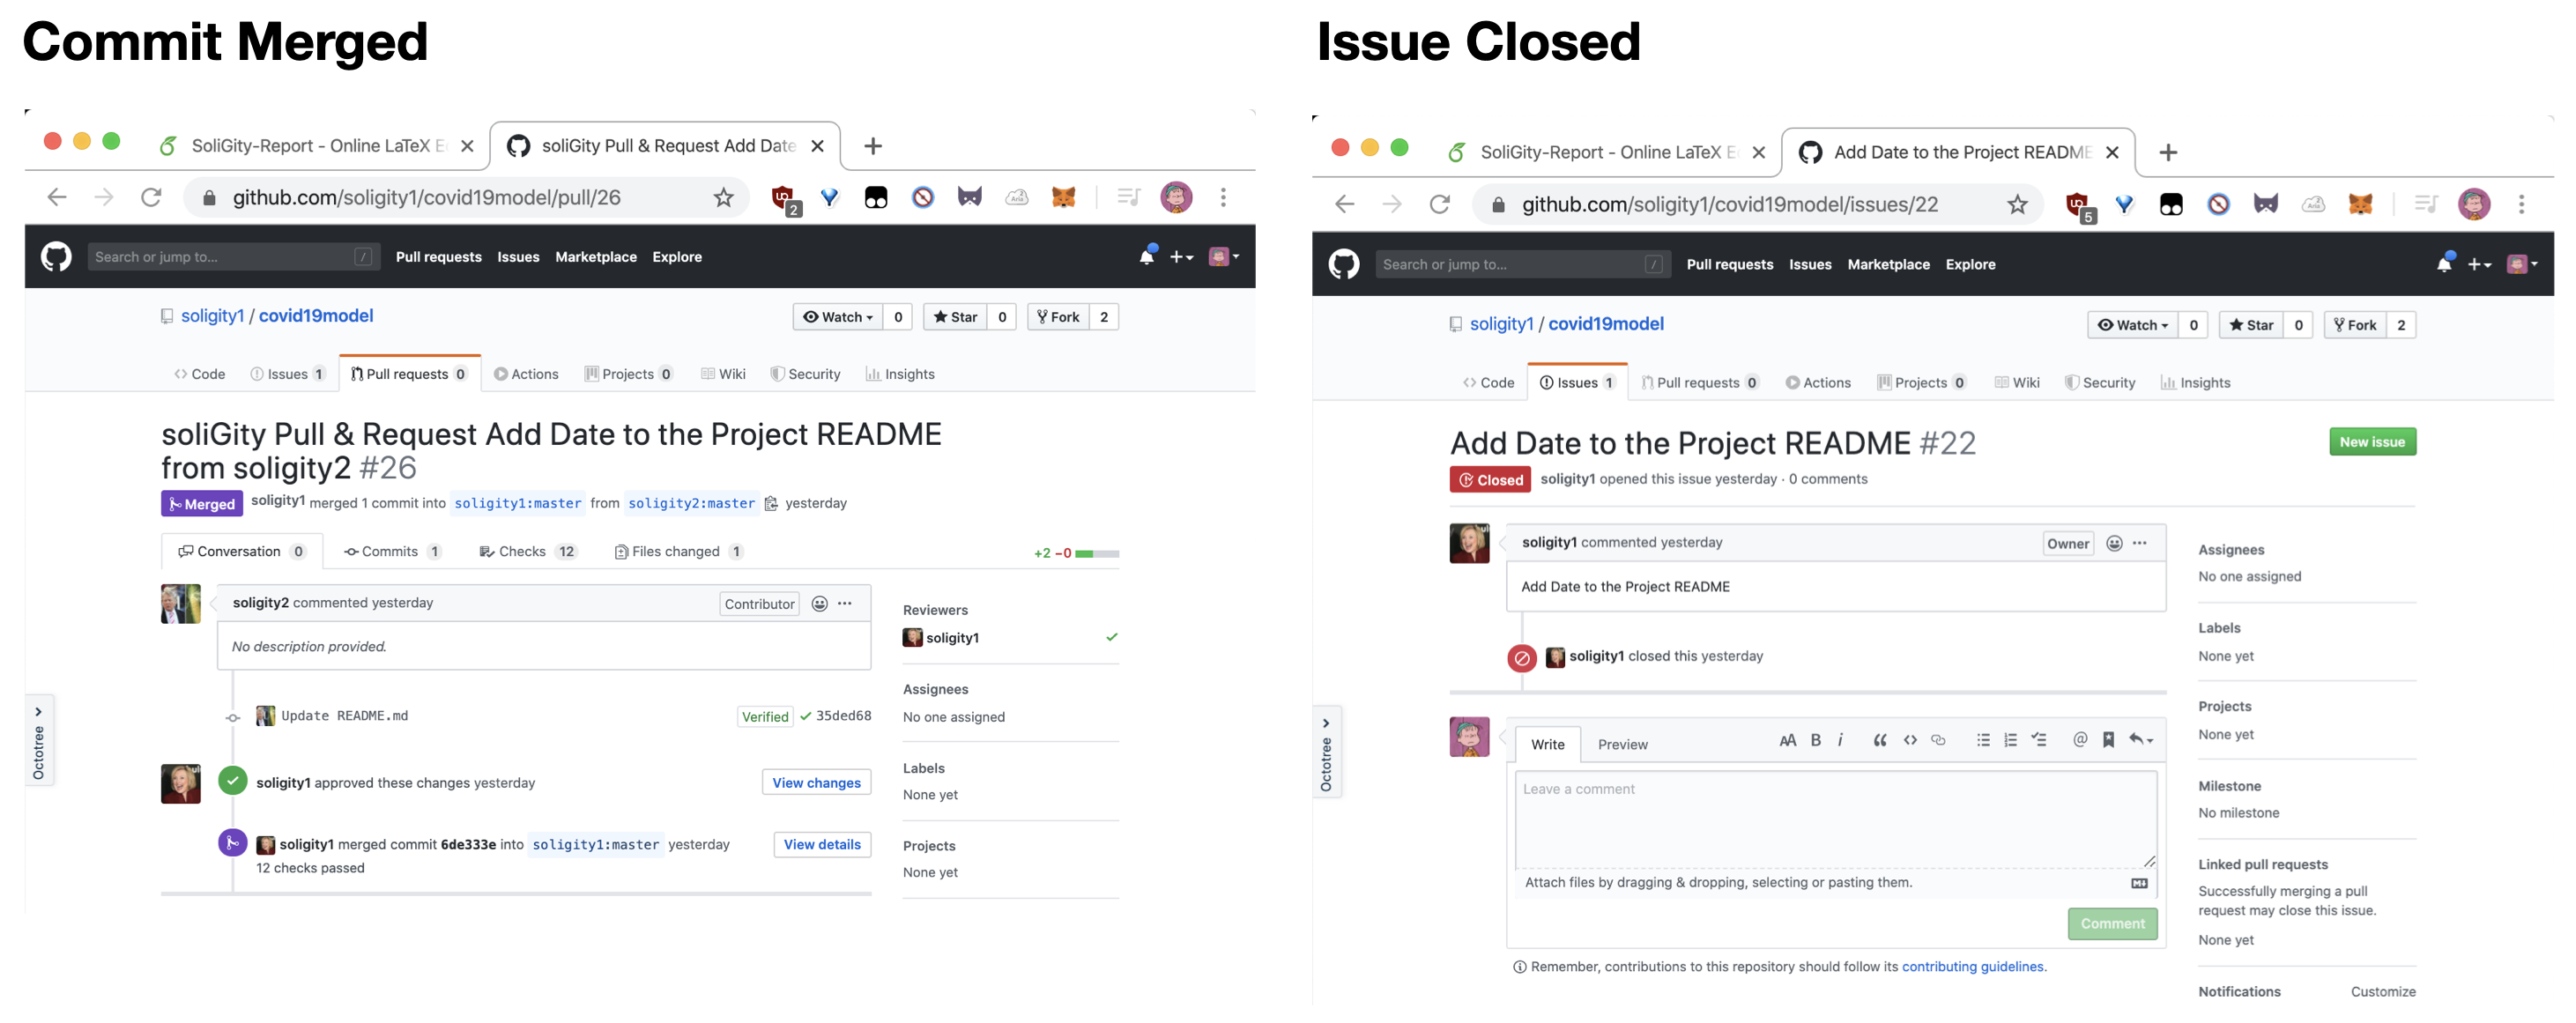
\includegraphics[width=16cm]{graphs/56. reward_3.png}\\
	\caption{Pull Request and Issue closed}
	\label{fig:reward3}
\end{figure}


% \begin{figure}[H]
% 	\centering
% 	\begin{subfigure}[b]{.45\textwidth}
% 		\centering
% 		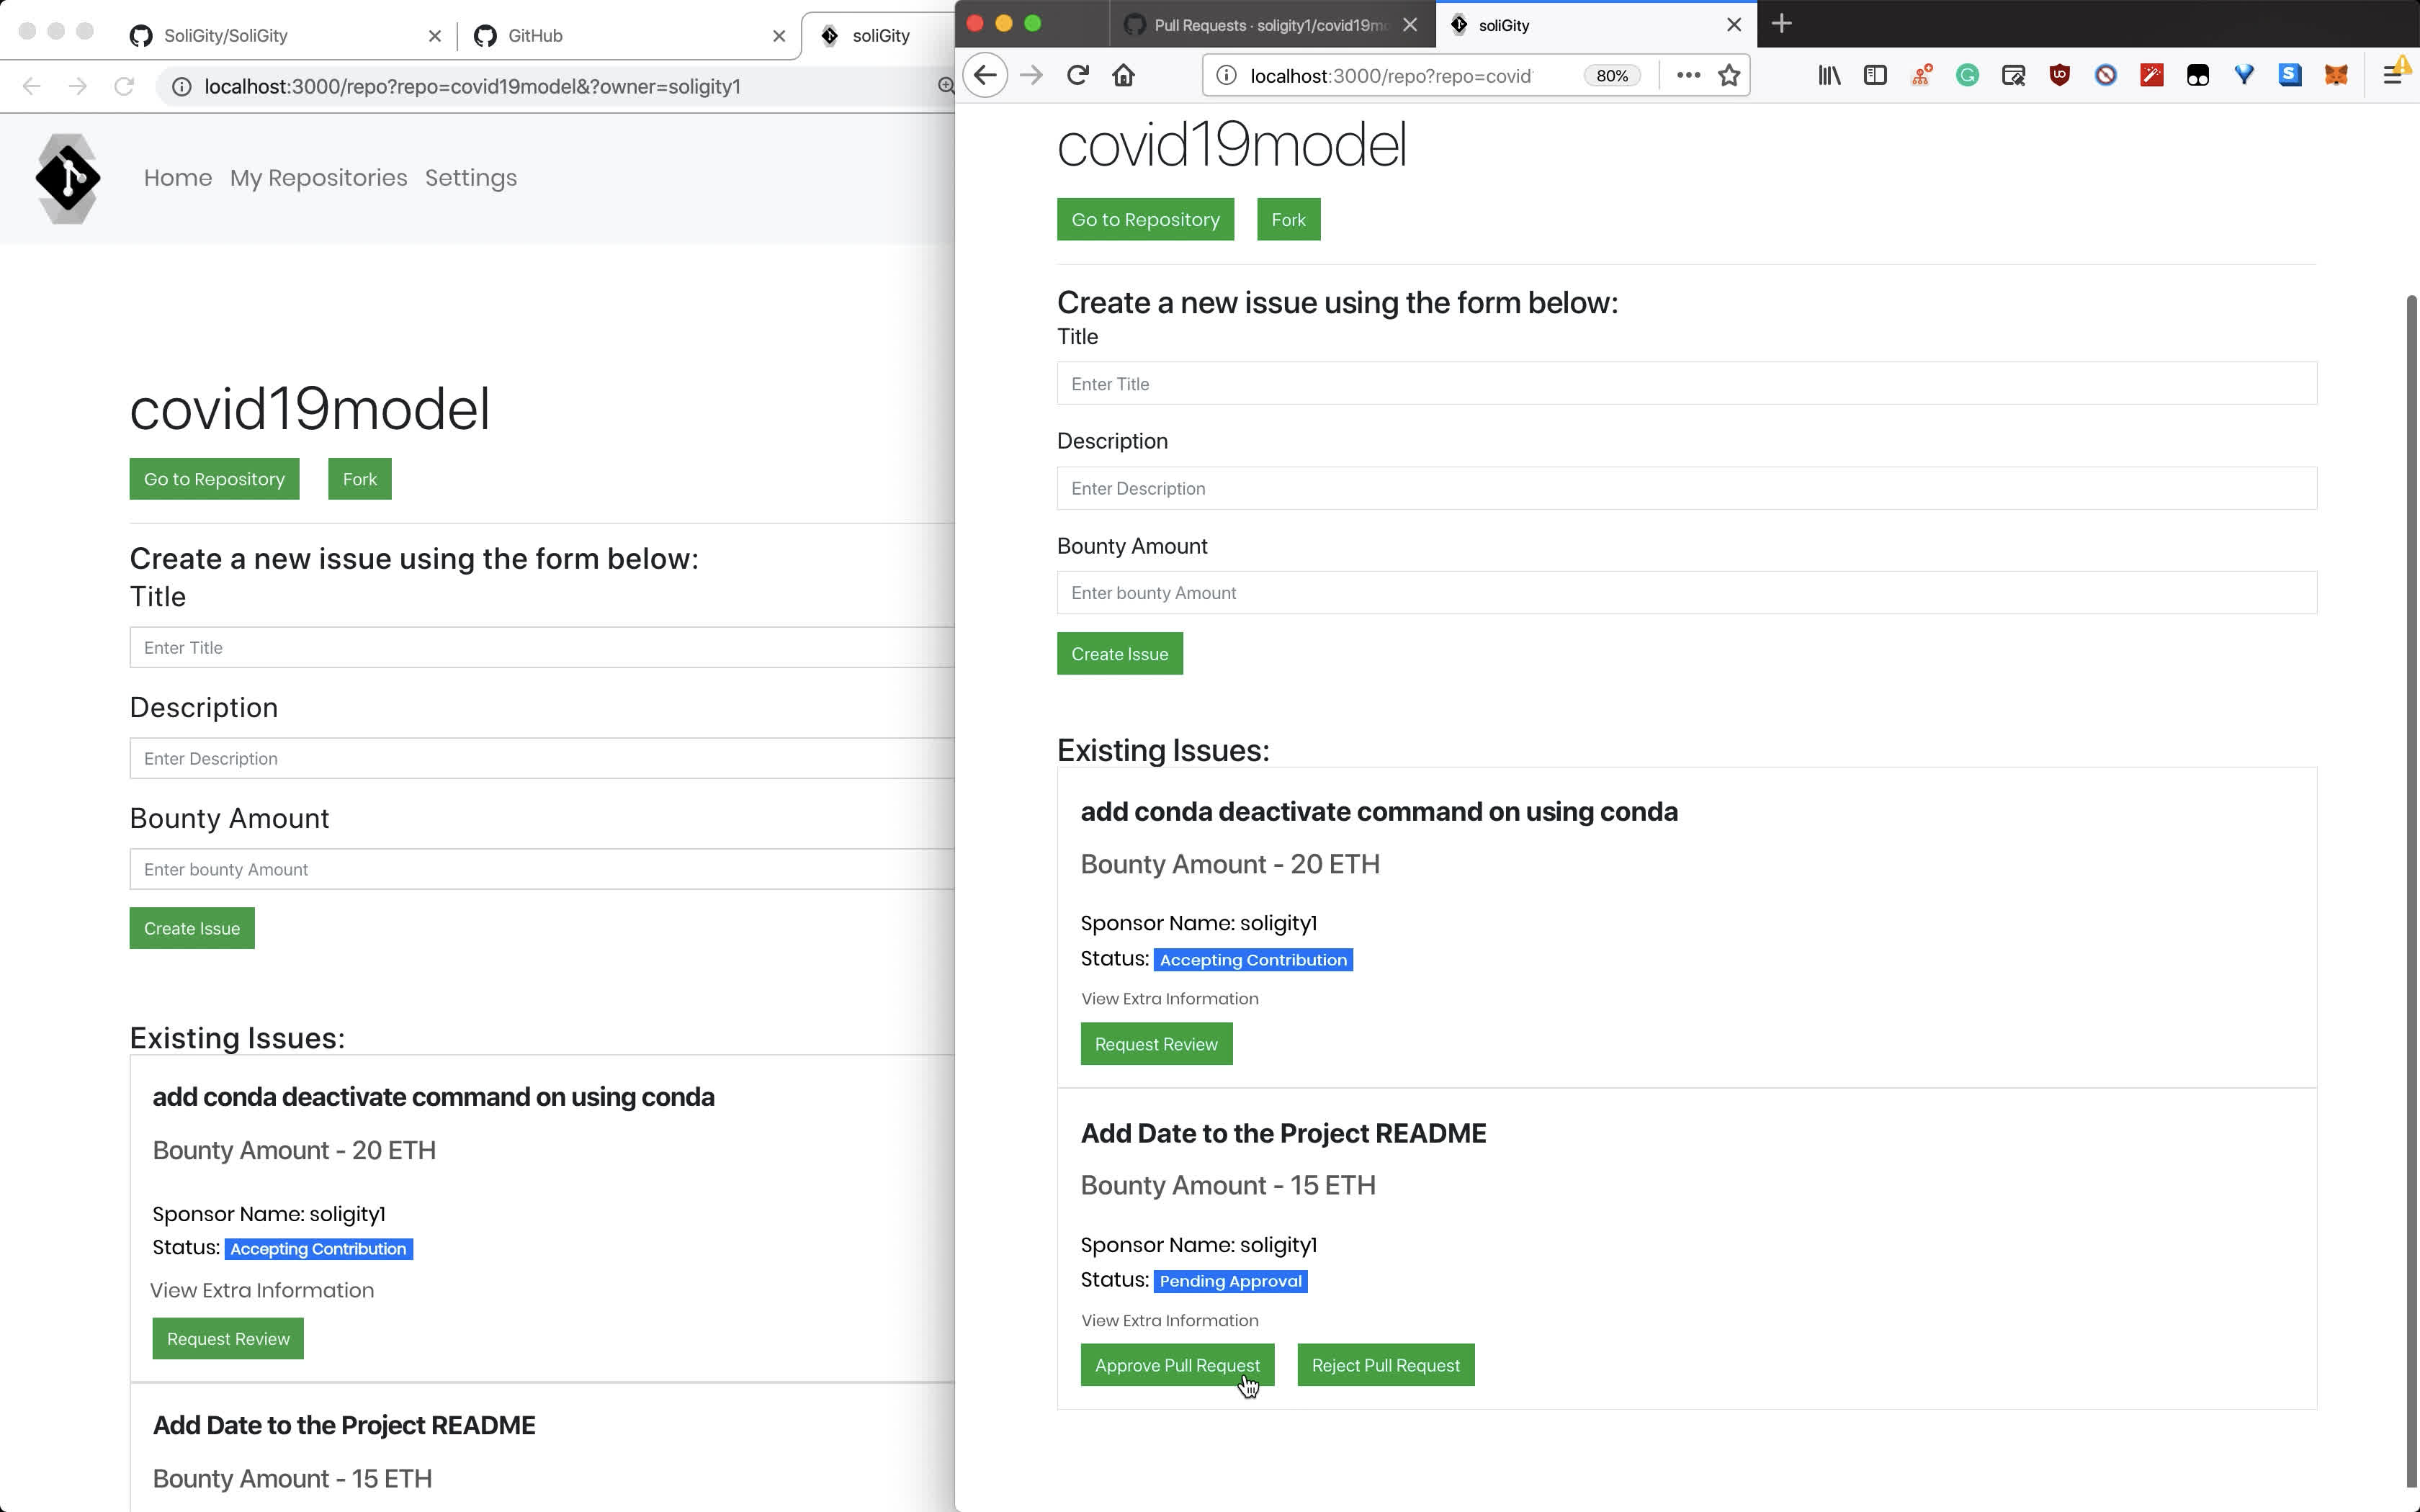
\includegraphics[height=4cm]{graphs/40. alice_approve_pull_request}
% 		% \caption{Alice Reject Pull Request}
% 	\end{subfigure}
% 	% \begin{subfigure}[b]{.32\textwidth}
% 	% 	\centering
% 	% 	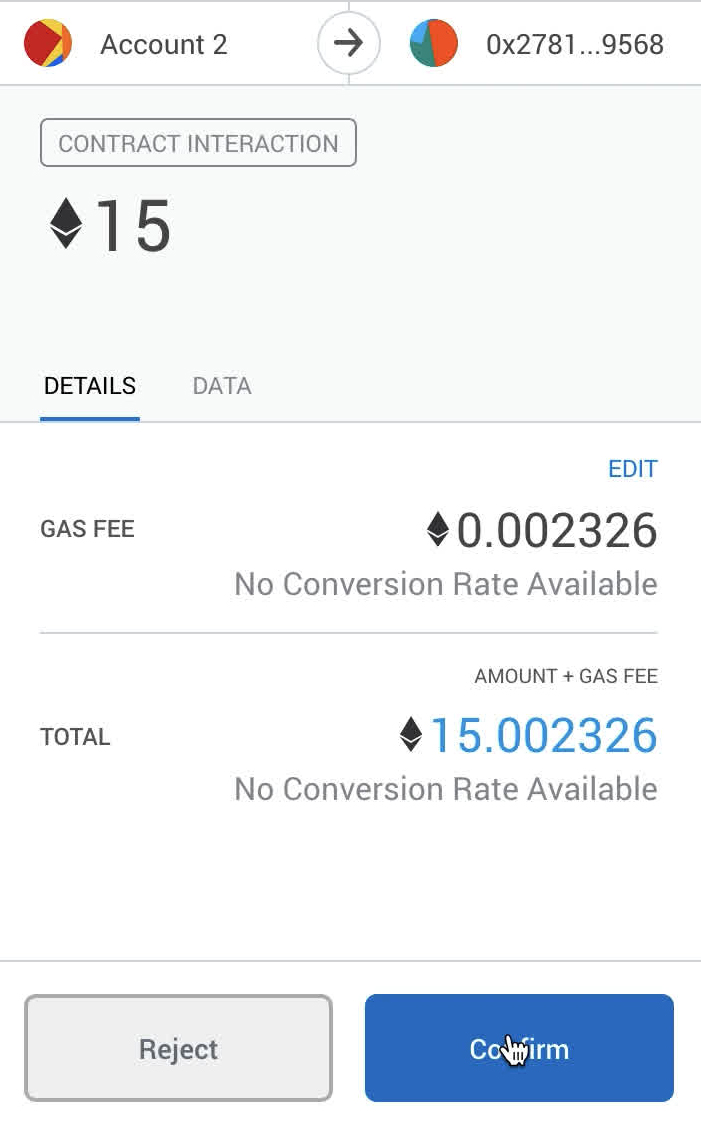
\includegraphics[height=5cm]{graphs/41. alice_metamask_confirm}
% 	% 	% \caption{Status}
% 	% \end{subfigure}
% 	\begin{subfigure}[b]{.45\textwidth}
% 		\centering
% 		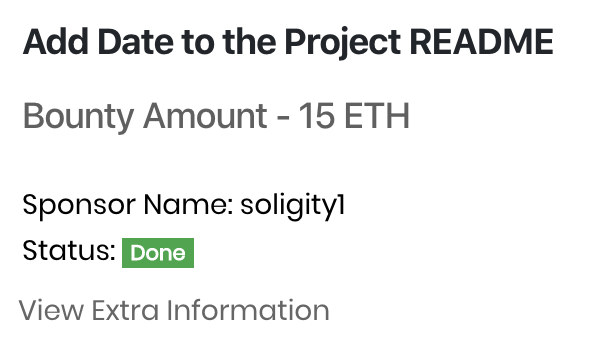
\includegraphics[height=4cm]{graphs/41. issue_status_done}
% 		% \caption{Status}
% 	\end{subfigure}
% 	\caption{Alice Approves Pull Request and the Status of Issue Becomes to \textit{Done}}
% \end{figure}

% \begin{figure}[H]
% 	\centering
% 	\begin{subfigure}[b]{.45\textwidth}
% 		\centering
% 		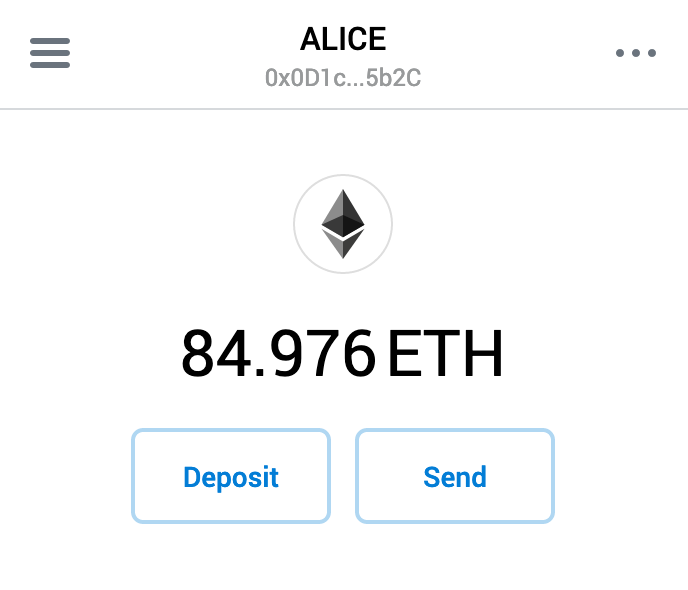
\includegraphics[height=4cm]{graphs/42. metamask_alice_balance}
% 		% \caption{Alice Reject Pull Request}
% 	\end{subfigure}
% 	\begin{subfigure}[b]{.45\textwidth}
% 		\centering
% 		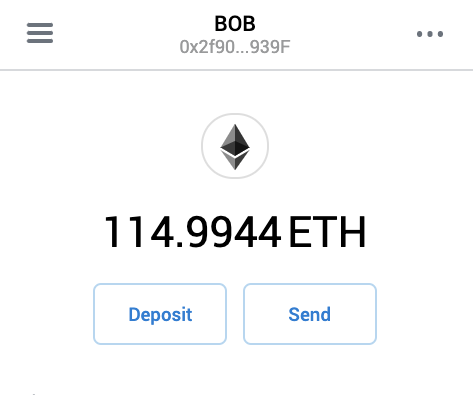
\includegraphics[height=4cm]{graphs/43. metamask_bob_balance}
% 		% \caption{Status}
% 	\end{subfigure}
% 	\caption{Changes in Balance of Alice and Bob}
% \end{figure}

% \begin{figure}[H]
% 	\centering
% 	\includegraphics[height=7cm]{graphs/42. alice_balaSnce_updated}
% 	\caption{Ganache Deployed Contracts}
% \end{figure}

% \begin{figure}[H]
% 	\centering
% 	
\includegraphics[height=7cm]{graphs/43. bob_balance_updated}
% 	\caption{Ganache Deployed Contracts}
% \end{figure}

% \begin{figure}[H]
% 	\centering
% 	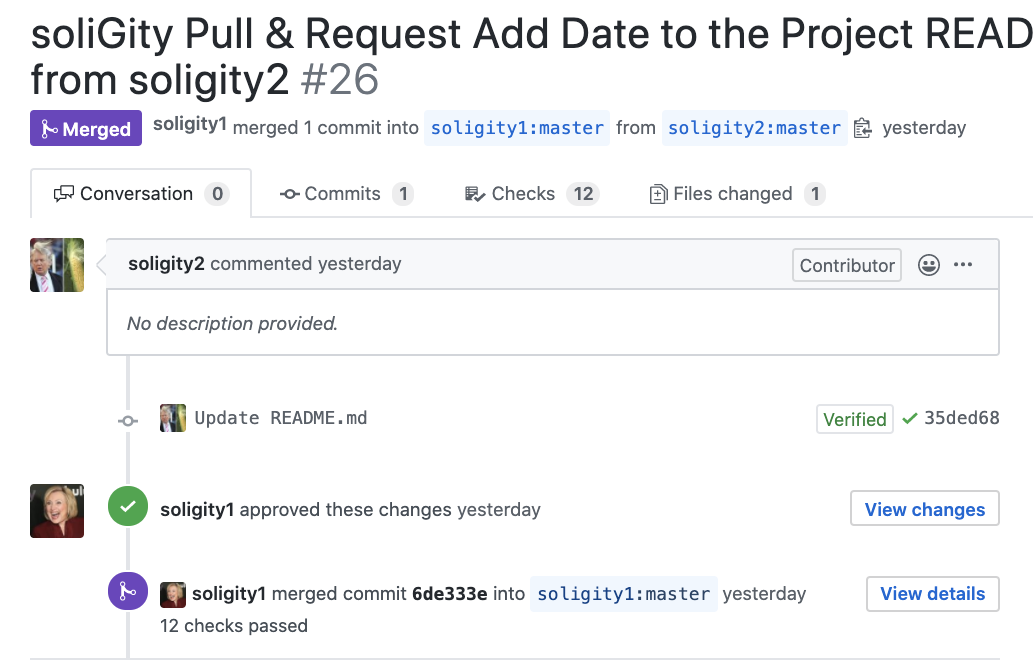
\includegraphics[height=5cm]{graphs/44. pull_request_closed}
% 	\caption{Pull Request Merged in the GitHub}
% \end{figure}

% \begin{figure}[H]
% 	\centering
% 	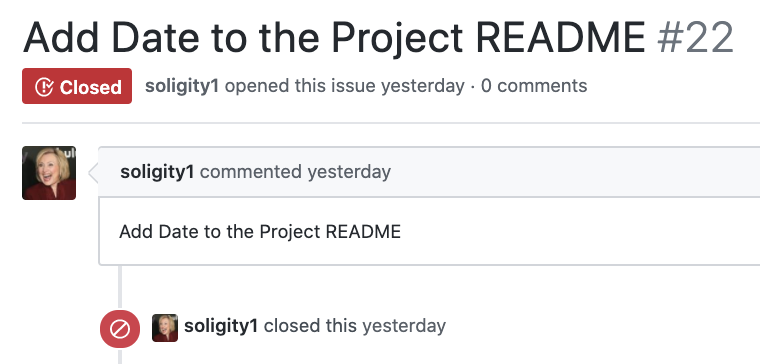
\includegraphics[height=4cm]{graphs/45. issue_closed}
% 	\caption{Issue Closed in the GitHub}
% \end{figure}


\renewcommand\thesection{\arabic{section}}
\renewcommand\thesubsection{\thesection.\arabic{subsection}}

\section{Reflection}
From a technical standpoint, one significant challenge is to integrate Git into our application, this includes GitHub Connection to create issues, closing issues, forking repositories, creating pull requests, approving and merging pull requests, and reject pull requests, octokit/rest.js \url{https://octokit.github.io/rest.js/v17/}, and manually inputting GitHub username and password in the SoliGity to establish the connection. We created 2 GitHub test accounts to test out the relevant GitHub APIs to ensure they work properly. Another trivial but necessary work is to make sure the website prompts for user account and store the information in the backend. We define endpoints in the backend server, like creating new username, updating user info, and various GitHub actions mentioned above so that the request can be sent from frontend to backend APIs.

We made it possible that after logging in and associate their individual GitHub Account, users are able to obtain separate lists of their own repositories, which are only visible to themselves. However, once users are logged into the web page, we immediately realized that we need a solution to make sure that \textit{all} users have equal access to the Project Catalog. By reflecting the advantages of blockchain and smart contracts such as decentralization and transparency, we realize that this problem can be solved by saving project's information such as project owner, name, URL, etc. to the blockchain using Solidity smart contract and then propagate the list of projects in the SoliGity contract to the web page. Therefore, in addition to the transactions behind the rewarding mechanism, the Project Catalog page also takes advantage of blockchain technology, making it a true DApp.

One important takeaway of this project is problem identification: the most challenging, and most important stage of a project is to identify the right problem, before looking for solutions. Especially for technologies like Blockchain, a lot of the use cases and applications are remain unknown or underdeveloped. We started by asking ourselves how this technology can solve problems that we, as students, are likely to encounter at university. By relating to ourselves as well as surveying our peers, it seems obvious to us that most of us have had a challenging time getting prepared for the job market. As most of us have been working on software projects with Git source control, \textit{what would happen if we combine that with blockchain?} This question is followed by several rounds of discussions and refinements that finally becomes the working prototype of SoliGity. 

During the execution of the project, we also faced challenges in communication - due to the COOVID-19 pandemic, all of the work had to happen remotely, and the lack of face-to-face conversation in front of a whiteboard made it inconvenient to communicate some details about the implementation. This caused some asynchronous communications between members. For example, as GitHub is an asynchronous collaboration tool - when one person started working on the project, everyone else cannot obtain real-time updates and provide immediate feedback until the commit was pushed to the remote repository. Therefore, we had to go back and forth to make sure the design and implementation are well aligned. On the other hand, if we incorporated peer-programming, the efficiency would be reduced as members cannot work on the project simultaneously to increase the throughput. There is always a trade-off. On the plus side, however, our team developed a deep level of trust in each other from early on. We had honest conversations on each person's technical and non-technical strengths and effectively amplified these strengths. The result of our teamwork is a well-rounded product that packages an excellent level of strategic planning, technical uniqueness, practicality, aesthetics, branding, and execution.

Overall, this is a challenging, but rewarding experience that taught us technical, communication, and teamwork skills. We appreciate all the support and feedback that our professor and classmates have given.

\section{Future Work}
Here is a list of technical improvements that are in our roadmap:
\begin{enumerate}
    \item Support MetaMask Login \url{https://www.toptal.com/ethereum/one-click-login-flows-a-metamask-tutorial}
    \item  Github OAuth Login \url{https://medium.com/front-end-weekly/use-github-oauth-as-your-sso-seamlessly-with-react-3e2e3b358fa1} and \url{https://developer.github.com/apps/building-oauth-apps/authorizing-oauth-apps/}
\item To get rid of centralized database, which saves user information in the backend, achieve fully 
decentralized app.
\item Support more platforms that Support software development version control using Git.
\item To support more github actions in the soligity, like leave some comment in the participant's pull request, tell paritipant how to improve their works, instead of rejecting directly.
\item To enrich the content of our Project Catalog page by incorporating multimedia such as pictures, videos, etc. so that it will provide a higher fidelity project browsing experience similar to an App Store to attract people to work on open source projects.
\end{enumerate} 

Our existing prototype only allows one developer to claim an issue - once an issue is claimed by one contributor, no one else is allowed to make commitments. In the long term, we need to upgrade our smart contract to be able to support more than one request review. This is because in reality, a popular project may attract thousands of developers to do one task. More sophisticated rewarding mechanisms can be incorporated to help the owner decide and send the bounty to those who deliver the highest quality work. This is like a call-for-tender process, and will create a health competition among developers and motivate them to deliver their best share of work.

In addition, we wish to establish a connection between the project owner and company recruiters in addition to sending the incentive to contributors. This allows the developer to receive additional recognition that can potentially lead them to their dream jobs.  

Finally, our team will also need to study how to deploy the contract in the Ethereum’s main network and design tasks to find out potential risks (such as hackers that try to bypass system requests) in our contracts to avoid system failures.

\section{Value Proposition and Strategic Planning}
The objective of our work is simple: Create a secure, transparent, intuitive and trustworthy platform to establish a multi-win situation in the software-driven world. With seamless integration of blockchain technology and Git, SoliGity helps developers discover interesting projects to work on and get rewarded and recognized; helps project owners to utilize global talents to accelerate software development; helps companies identify talents through direct referral (future work). We also strive for excellent user experience by executing deployment tests and continuously collecting feedback to improve. 

We wish our solution to reach and benefit as many people as possible, therefore the service should be robust and cost-friendly. With that being said, this project is going to be open-sourced and free to use. It will hopefully operate using the donation from the general public. To make this happen, we are actively attending business pitch events such as UBC-RBC Get-seeded events and Hackathons related to Blockchain and Human Resources to expose our project to a broader audience. Apart from obtaining financial aids by winning awards to build up our web infrastructure, this will allow us to establish healthy, long-lasting connections with people in Education, Finance, Business, Engineering, and Sciences and potentially create collaboration opportunities.

As we envision a large group of our users are entry-level developers and university students, our first step is to work with university Hackathon organizers and student teams to let us connect with their members in person to promote the product. We will also host campus events such as info-session and open houses to provide demos and answer questions. We will design posters with an easily-accessible QR code to make it easy for students to sign up. We also plan to reach out to university Co-op programs and career advising services to convince them to promote our product to students. We believe that a small-scale but high-quality adoption will eventually create a ripple effect to impact broader and more diverse communities. 

\newpage


\begingroup
\raggedright

\bibliography{mybib.bib}{}
\bibliographystyle{unsrt}
\nocite{*}

\endgroup

\newpage

\begin{appendices}

	\section{Course Project Team Form}

	\begin{center}
		\textbf{Team Name: \uline{\hspace{10em}}}
	\end{center}

	\begin{table}[H]
		\centering
		\begin{tabular}{| C{2cm} | C{4cm} | C{4cm} | C{4cm} |}
			\hline
			\textbf{Index} & \textbf{Student No.} & \textbf{First Name (Printed)} & \textbf{Last Name (Printed)} \\ \hline
			1              &                      &                               &                              \\ \hline
			2              &                      &                               &                              \\ \hline
			3              &                      &                               &                              \\ \hline
			4              &                      &                               &                              \\ \hline
			5              &                      &                               &                              \\ \hline
		\end{tabular}
	\end{table}

	\begin{table}[H]
		\centering
		\begin{tabular}{| C{2cm} | C{6cm} | C{6cm} |}
			\hline
			\textbf{Index} & \textbf{Signature} & \textbf{Date} \\ \hline
			1              &                    &               \\ \hline
			2              &                    &               \\ \hline
			3              &                    &               \\ \hline
			4              &                    &               \\ \hline
			5              &                    &               \\ \hline
		\end{tabular}
	\end{table}
	\newpage

	\section{Course Project Peer-to-Peer Evaluation Form}

	\begin{center}
		\textbf{Team Name: \uline{\hspace{10em}}}
	\end{center}

	\begin{table}[H]
		\centering
		\begin{tabular}{| C{2cm} | C{4cm} | C{4cm} | C{4cm} |}
			\hline
			\textbf{Index} & \textbf{Student No.} & \textbf{First Name (Printed)} & \textbf{Last Name (Printed)} \\ \hline
			1              &                      &                               &                              \\ \hline
			2              &                      &                               &                              \\ \hline
			3              &                      &                               &                              \\ \hline
			4              &                      &                               &                              \\ \hline
			5              &                      &                               &                              \\ \hline
		\end{tabular}
	\end{table}

	\begin{table}[H]
		\centering
		\begin{tabular}{| C{2cm} | C{4cm} | C{4cm} | C{4cm} |}
			\hline
			\textbf{Index} & \textbf{Percentage} & \textbf{Signature} & \textbf{Date} \\ \hline
			1              &                     &                    &               \\ \hline
			2              &                     &                    &               \\ \hline
			3              &                     &                    &               \\ \hline
			4              &                     &                    &               \\ \hline
			5              &                     &                    &               \\ \hline
		\end{tabular}
	\end{table}
	\newpage

\end{appendices}

\end{document}